

	\chapter{Architectural description}
		\section{Overview}
			\paragraph{}
				The product is a distributed application based on the three logic layers of
				\begin{quote}
					\begin{description}
						\item[Presentation] manages the user's interaction with the system
						\item[Application] handles the logic of the system
						\item[Data] manages the information.
					\end{description}
				\end{quote}				 
			\paragraph{}
				Those three layers are divided onto four different physical tiers. As shown in \ref{fig:tiers}, Presentation and Data levels reside on a single tier, while Application level is split into two tiers (Web Server and Application Server). The Web Server is in charge of serving static assets and of forwarding API requests to the Application Server, which in turn implements the business logic of the application.
				\begin{figure}[!h]
					\centering
					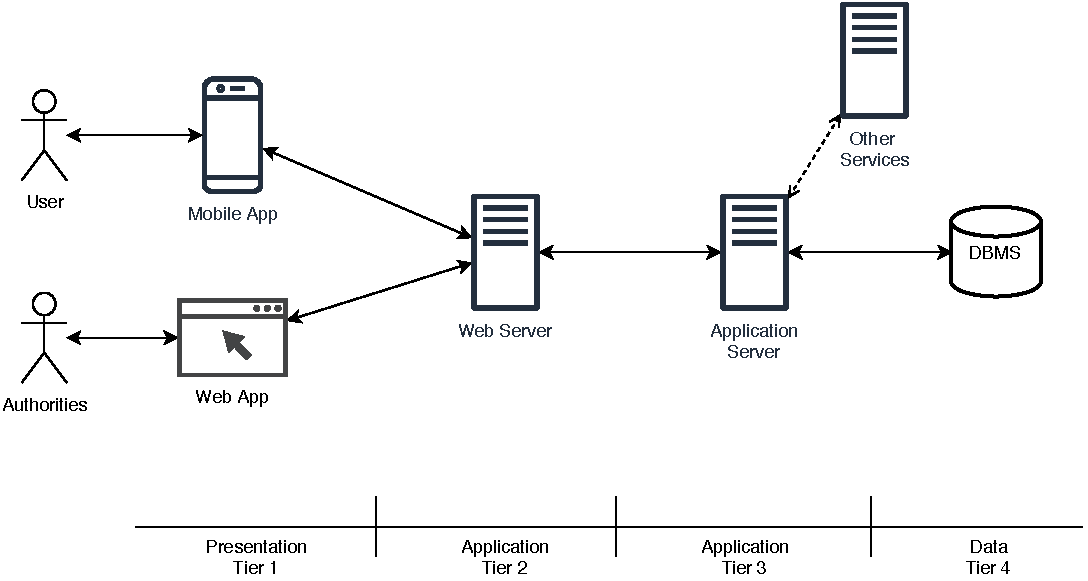
\includegraphics[width=\textwidth]{images/DD2/SimplifiedDeploymentView.pdf}
					\caption{Layers and tiers diagram}
					\label{fig:tiers}
				\end{figure}
			\paragraph{}
				In order to maximize the scalability of the system, both the Web and Application servers follow a scale-out approach: performances improvement is obtained through nodes replication. Because of this approach, load-balancing system are used in order to distribute the working load among the various nodes. 
				
				All the nodes of the Application Server use a "share everything" configuration, because there is only one shared database with one point of access. 
				
				Moreover, the Data layer is accomplished by exploiting an external DBMS service already available on the market. In this way we avoid devoting time on difficult problems about data replication and consistency, which are already solved by the existing and well tested database systems.
			\paragraph{}
				Every communication channel is secured by using firewalls. In this way, the Web Server is secured in a DMZ while Application Server protected as part of the LAN, so attacks and intrusions from malicious  clients will be prevented. It is important to note that, because the DBMS is located on a different tier with respect to the Application Server, a firewall between them can improve the security of the system.
				
				Finally, communication channels between the Application server and other services, like the Ticket Service, are secured for the same reasons explained above.
				\begin{figure}[!h]
					\centering
					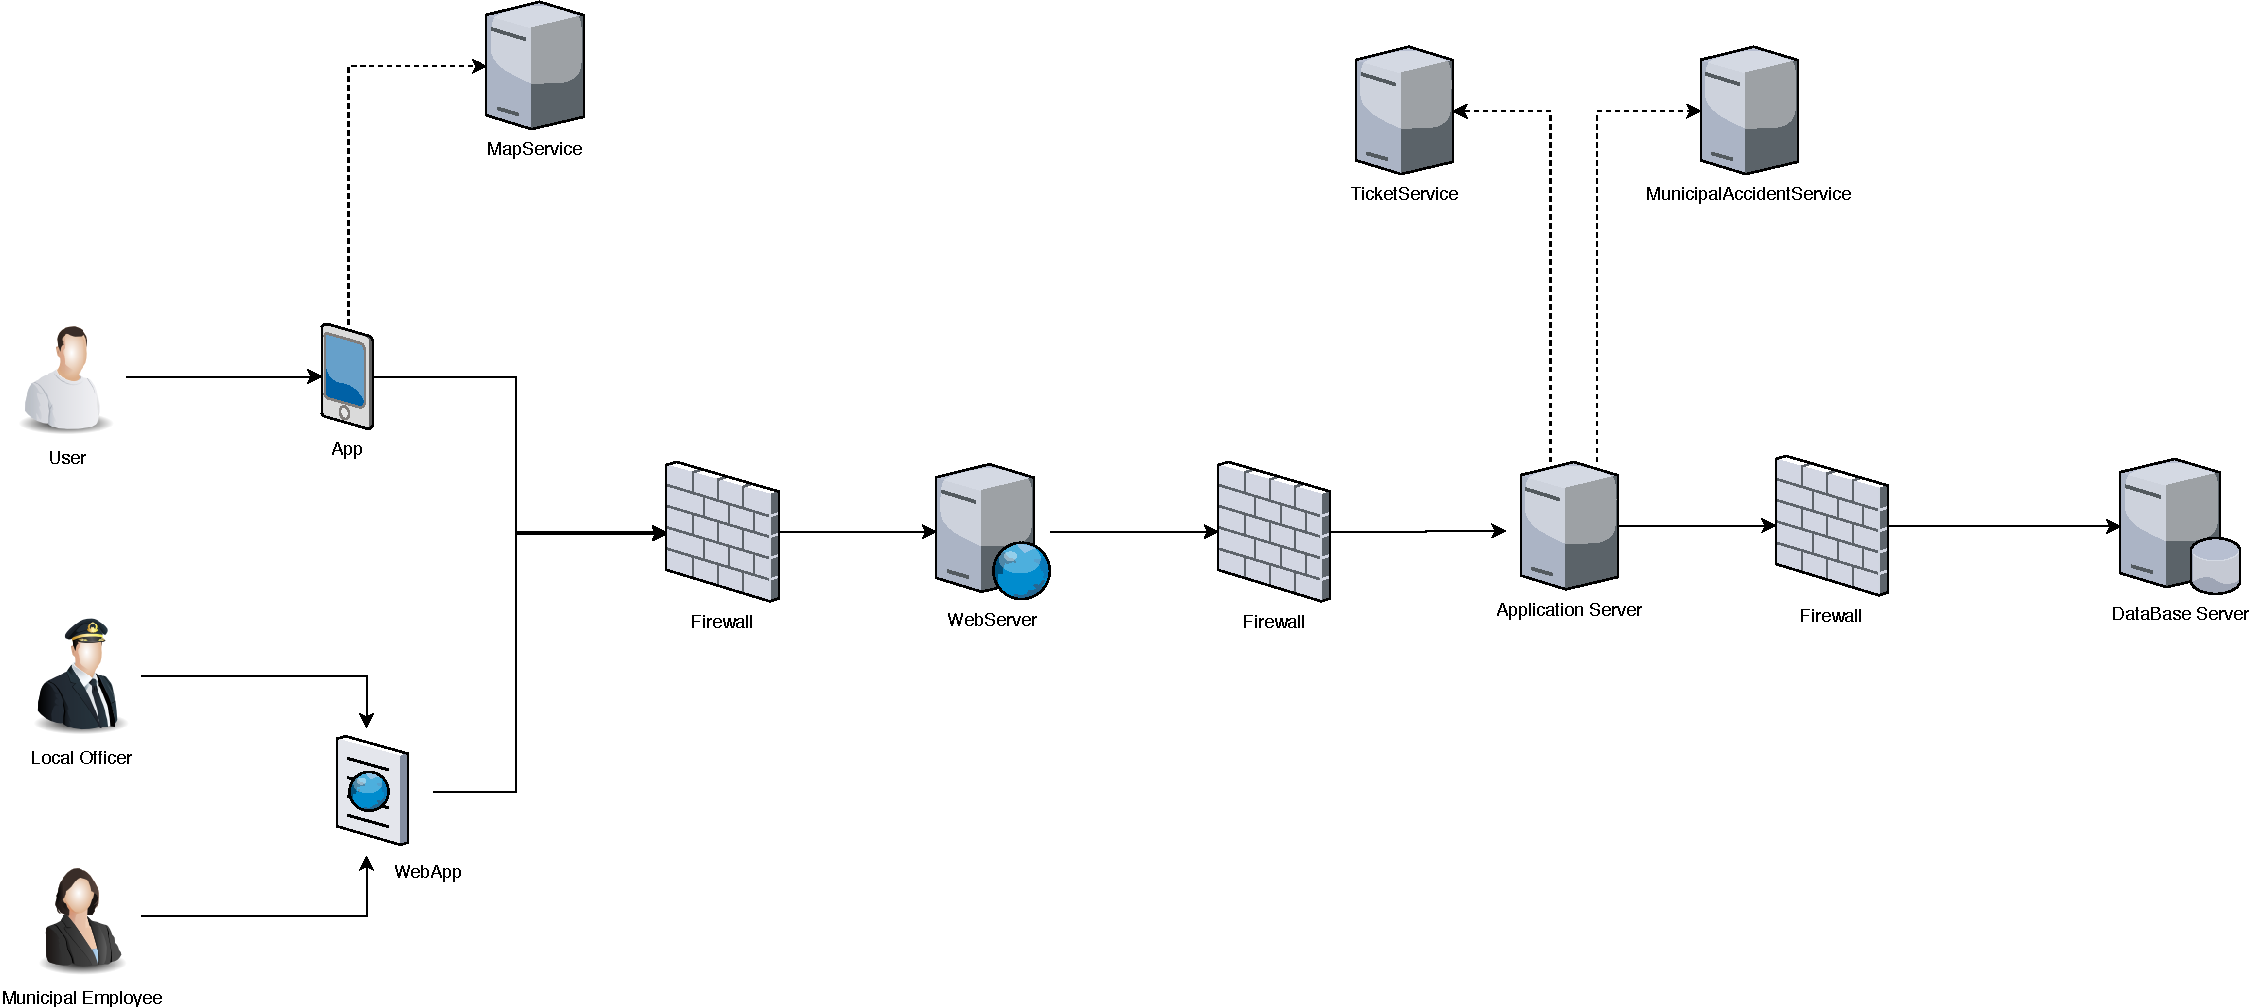
\includegraphics[width=\textwidth]{images/DD2/SystemArchitecture.pdf}
					\caption{System architecture}
				\end{figure}
		\clearpage
		\section{Component view}
			\begin{figure}[!h]
				\centering
				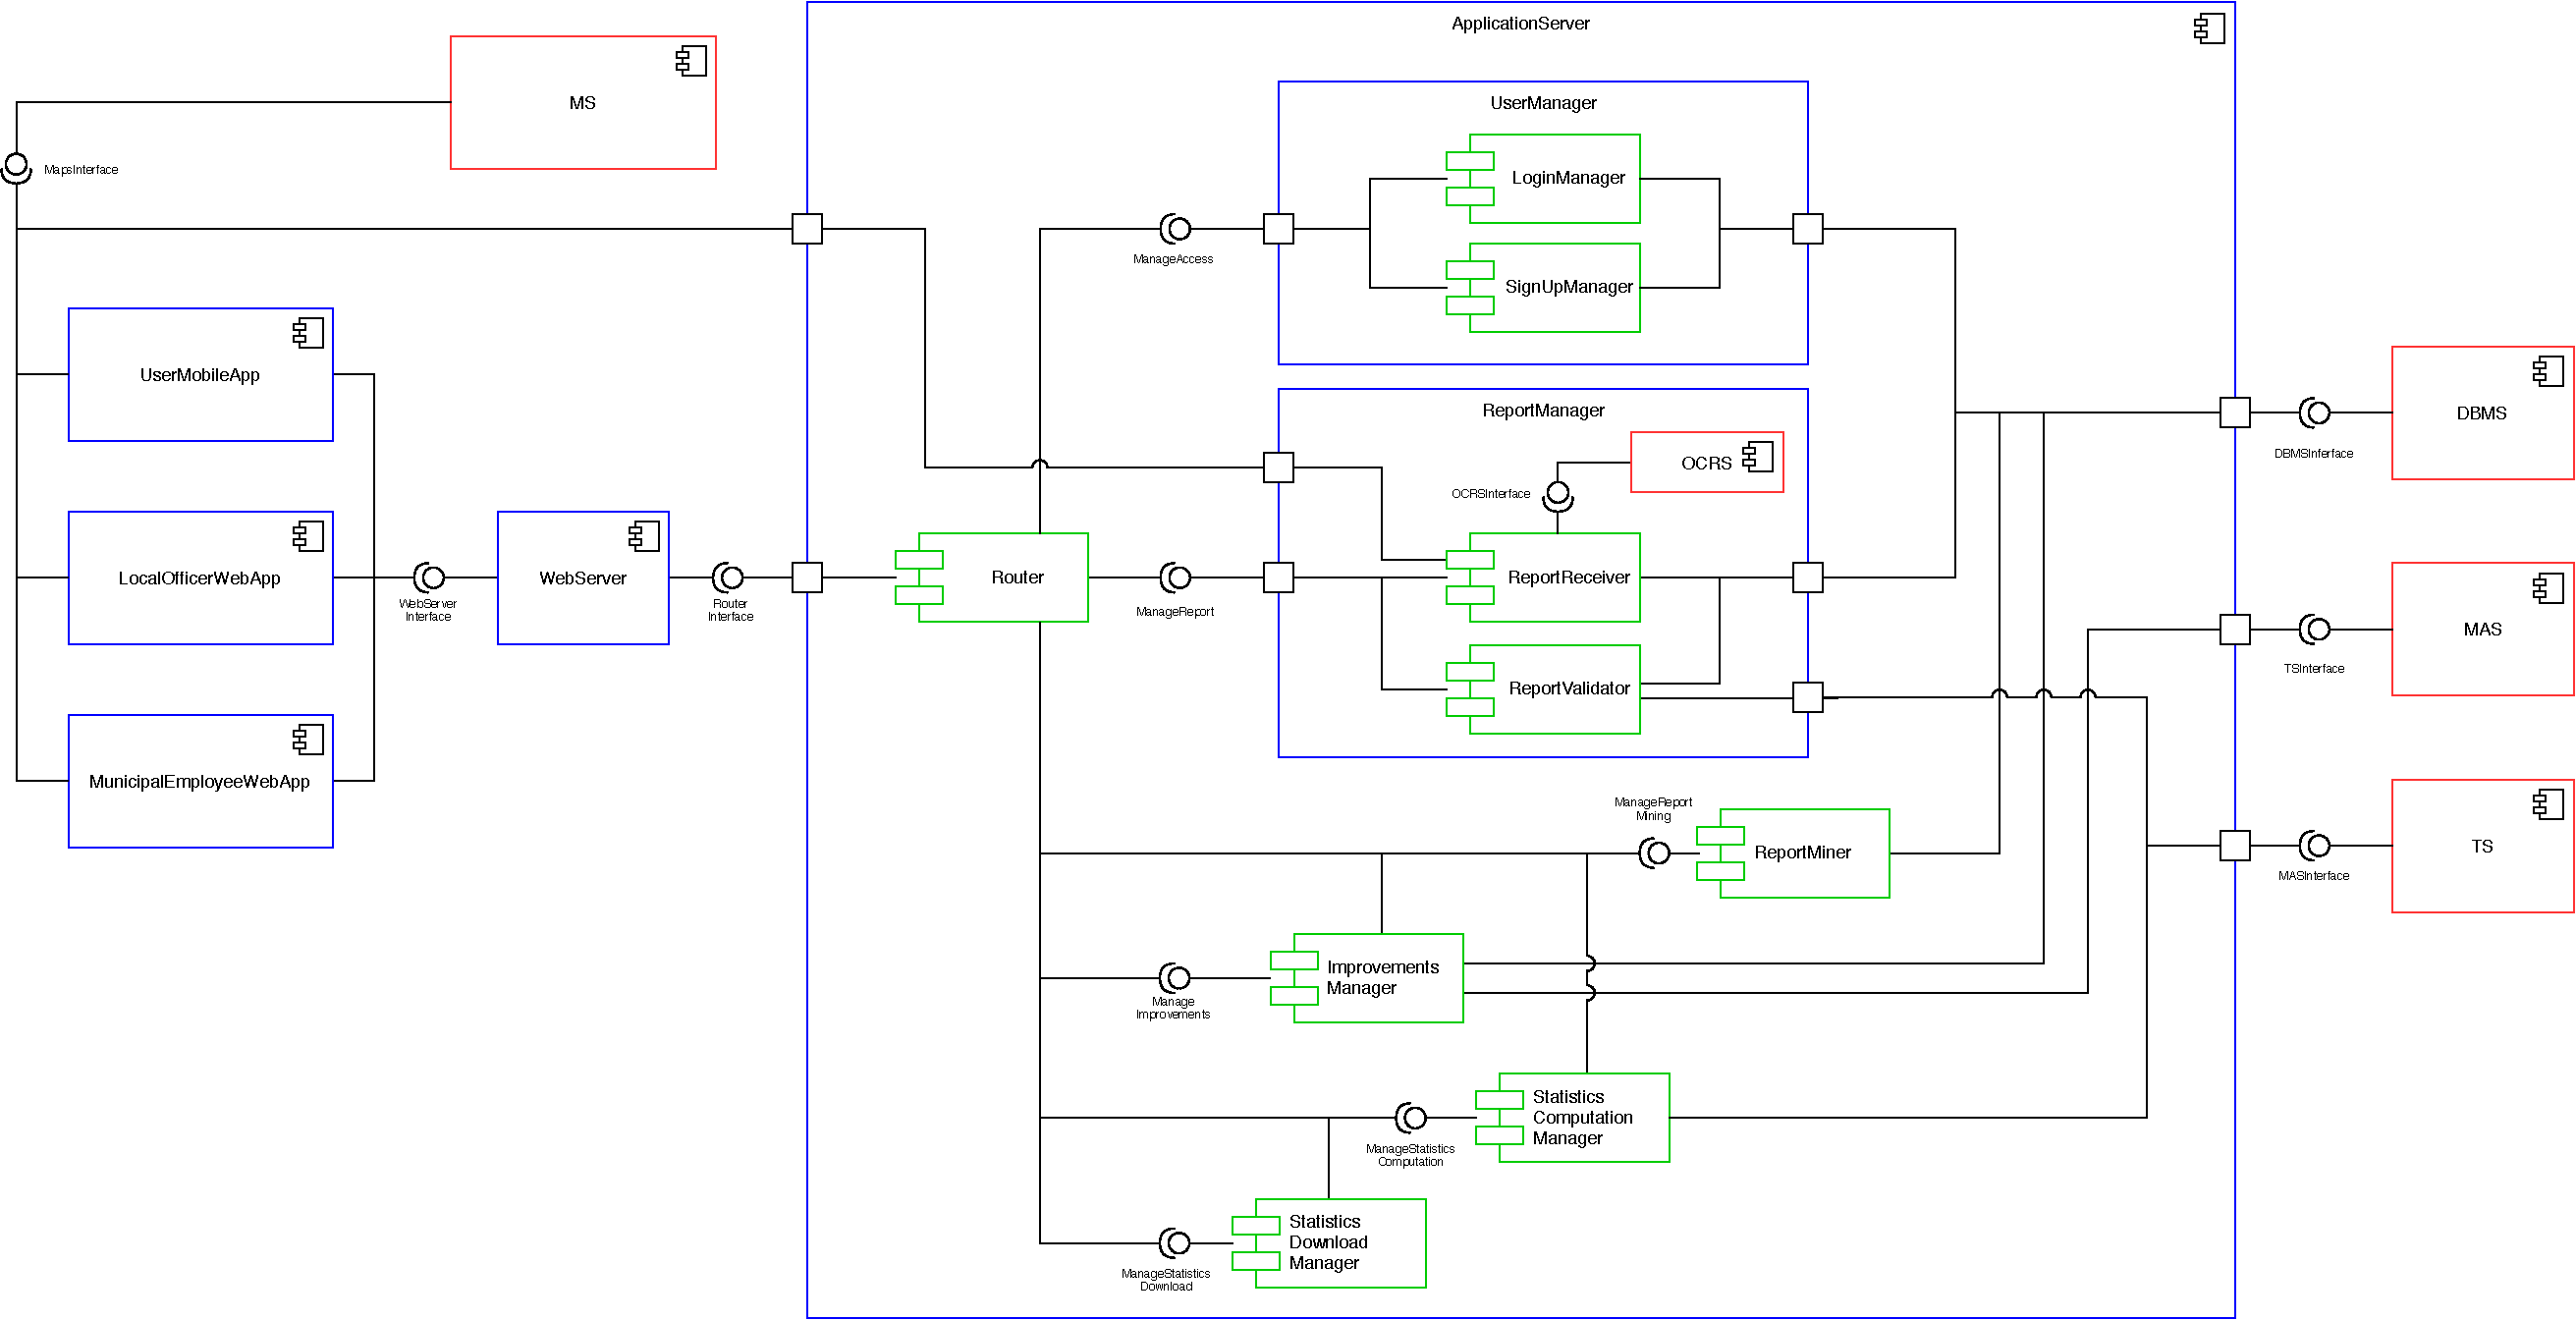
\includegraphics[width=\textwidth]{images/DD2/ComponentDiagram.pdf}
				\caption{Component view diagram}
			\end{figure}
			\paragraph{}
				The Component view diagram represents, explicitly, only the components of the Application server, as they depict the main section of the system. 
				Below, is describe in depth the function of every internal server component made ad-hoc for the system (the ones in green).
			\begin{description}
				\item[Router]: receives HTTP over SSL/TLS requests following the REST paradigm (see also \ref{sez:componentInterface}) and forwards them to the others internal components of the Application server. Then, it forwards the replies back to the clients. It is relevant to note that temporary tokens are adopted, in order to define which functionalities are accessible for each client. Every client receives its personal token after the login procedure. 
				\item[UserManager]: 
					\begin{itemize}
						\item \textbf{LoginManager}: this component is responsible for granting access to registered users. In particular, the component receives the access credentials and, if they are correct, it returns a unique token used for further communication by the user. otherwise it returns an error message
						\item \textbf{SignUpManager}:  this component is responsible for the registration of unregistered users. In particular it receives the new access credentials and, if they are acceptable, it saves them in the system's database, otherwise it returns an error message
					\end{itemize}
				\item[ReportManager]: 
					\begin{itemize}
						\item \textbf{ReportReceiver}: this component is responsible for receiving the data of new reports and storing them in the database. In particular it takes care of the following tasks:
							\begin{itemize}
								\item employ the MS APIs to retrieve the information about which municipality the report has been created from
								\item recognizing the vehicle's plate in the picture, by employing the OCRS APIs. In case of an unrecognizable plate, the report status will be set to "NOT VALID" by default and a NULL vehicle will be set, otherwise it will be "NOT VERIFIED" (which means that a Local Officer has still to prove its validity) and the correct vehicle is associated to the report
								\item saving the report in the system's database
							\end{itemize}
						\item \textbf{ReportValidator}: this component is responsible for two main operations:
							\begin{itemize}
								\item fetching, from the database, of reports with status set to "NOT VERIFIED"
								\item  modification of status of a set of report, by changing it from "NOT VERIFIED" to "VALID" or "NOT VALID" according to the request sent by the local officer. Then it saves them in the database and sends them to the TS (if set to "VALID"), responsible for issuing traffic tickets
							\end{itemize}
					\end{itemize}
				\item[ReportMiner]: this component is responsible for obtaining reports by querying the database. It is crucial to note that the request can come directly from the Router or from other components like the ImprovementsManager and StatisticsComputationManager. In both cases, the municipality (obtained by the authority requiring or from the position required) is used for filtering reports. Only reports with status set to "VALID" are fetched. Various form of mining can be performed, in particular it's is possible to mine:
					\begin{itemize}
						\item All: all the reports produced in the specific municipality, are returned
						\item By Type: between all the reports produced in the specific municipality only those which have the given violation's type are returned 
						\item By Date: between all the reports produced in the specific municipality only those which were composed on the given date are returned
						\item By Time: between all the reports produced in the specific municipality only those which were composed on the given time, regardless the date, are returned
						\item By Area: between all the reports produced in the specific municipality only those which were composed in the given area, defined by a center and a radius, are returned
					\end{itemize}
				In each case, if there are no reports satisfying the request, an error message is returned.
				\item[ImprovementManager]: this component is responsible for getting the possible improvements belonging to the requesting authority's municipality and for setting their status. In order to determine the possible improvements, it crosses the data coming from the external MAS and from the MineReports component. When a new improvement is determined, it's status is set by default to "NOT DONE" and it is saved in the database. When no further improvements can be discovered, all those which have the status set to "NOT DONE" are returned to the requester. Moreover, through this component, an authority can set the status of a specific improvement to "DONE", after fetching all the possible one as described before. 
				\item[StatisticsComputationManager]: this component is responsible for building statistics, belonging to the requesting authority's municipality, about the violations and the perpetrators who cause them, by crossing the information coming from reports received by the ReportMiner and from issued tickets coming from the TS. It is important to note that statistics are always crunched on request and never saved on the server, because they can change at any time.
				\item[StatisticsDownloadManager]:this component is responsible for creating a non-materialized document (which means it is not saved on server side, but only generated and sent) about the statistics, belonging to the requesting authority's municipality,  by fetching them from the StatisticsComputationManager. The resulting document is returned to the caller
				\item[QueryManager]: this component exploits database's functionality in order to offer simple interfaces to server's components
			\end{description}
		\section{Deployment view}
			\begin{figure}[!h]
				\centering
				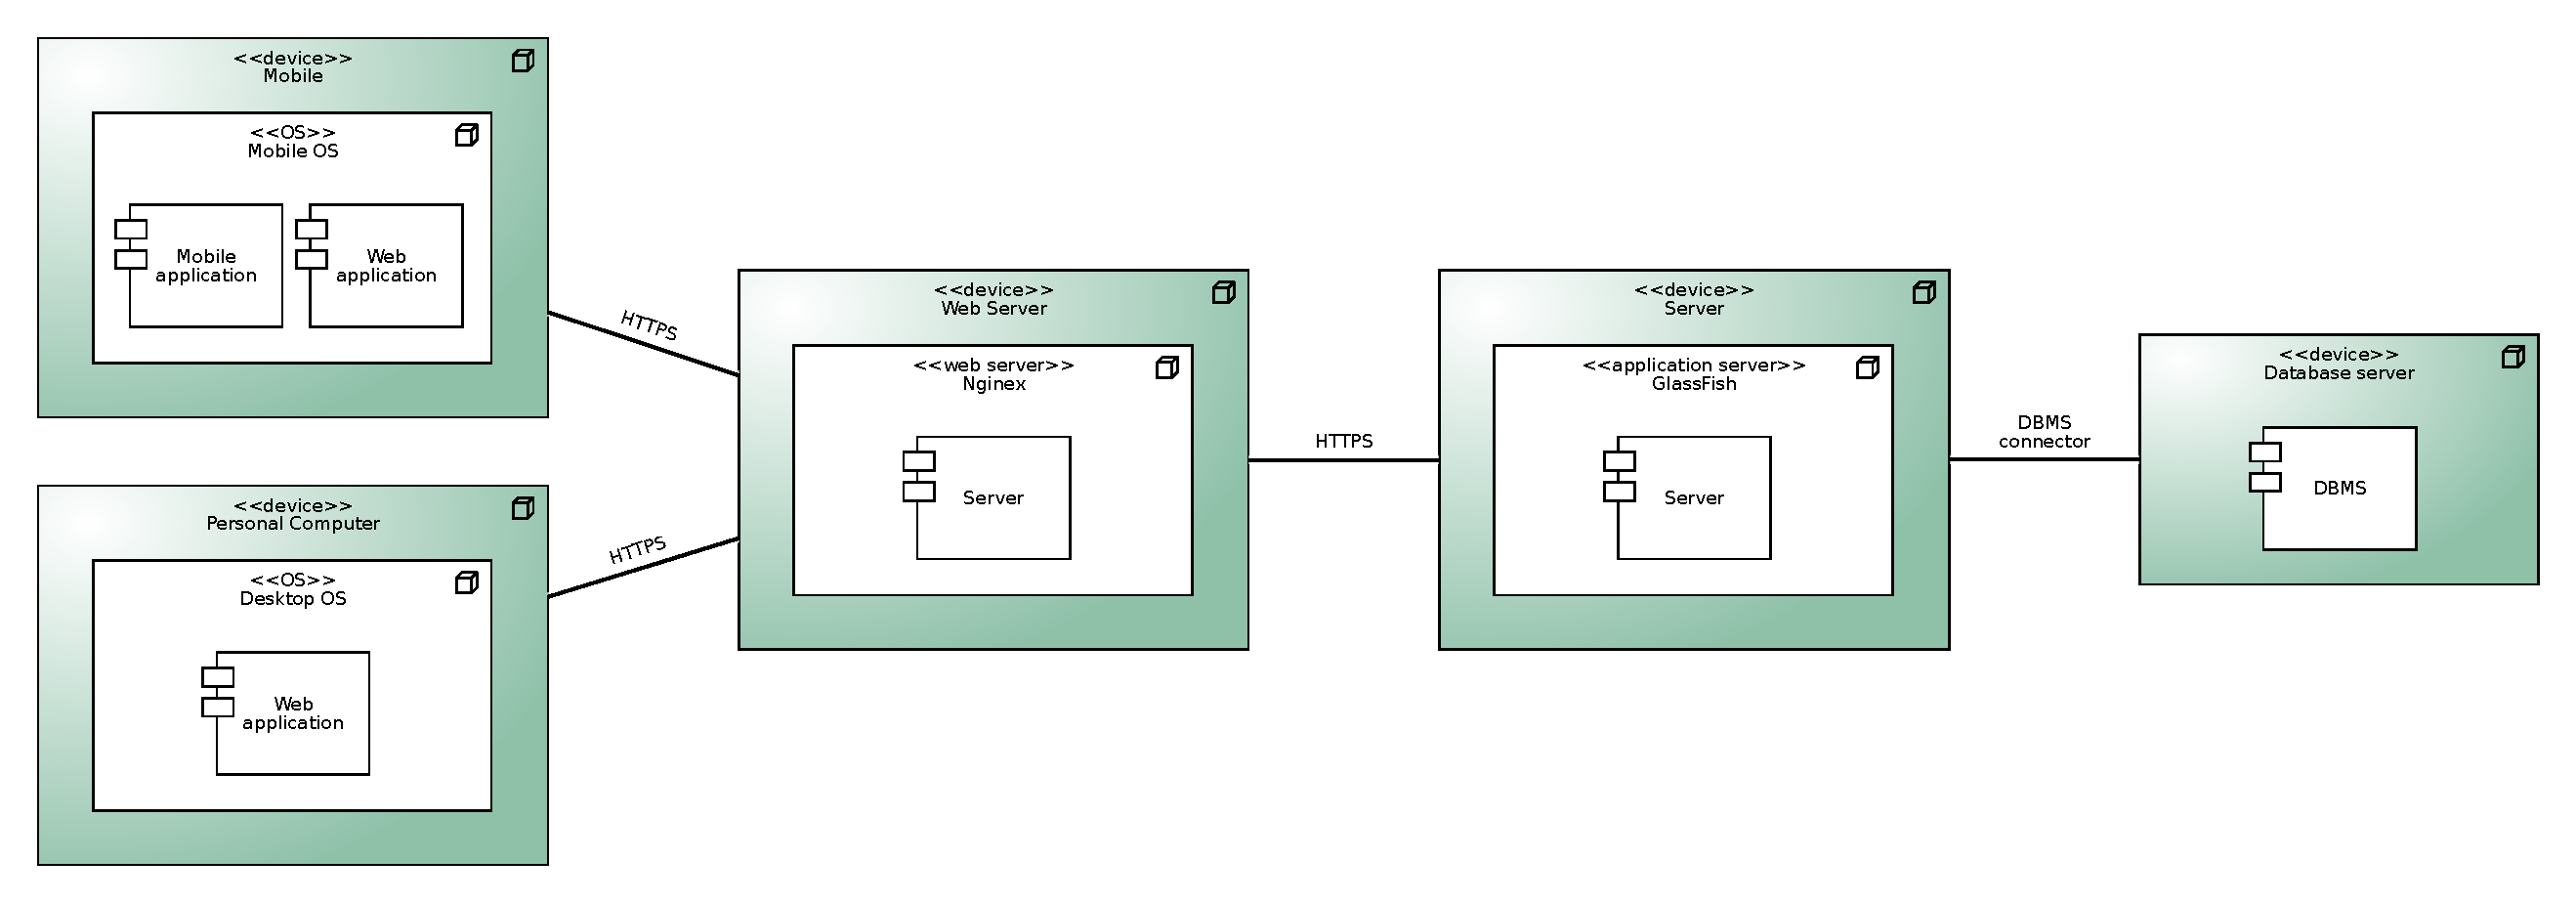
\includegraphics[width=\textwidth]{images/DD2/DeploymentView.pdf}
				\caption{Deployment view diagram}
			\end{figure}
			\paragraph{}
				This picture shows how the system should be deployed (ignoring external services):
				\begin{itemize}
					\item It is available for end users as a Mobile Application, while, for authorities, as a Web Application, accessible both from Mobile and PC (using a browser)
					\item The Web Server, deployed on its physical node, has the purpose of serving static assets without intervention by the Application Server. Any other request received from the clients (both the Web and Mobile application) is automatically forwarded to the Application Server
					\item The Application Server and the Database Server are deployed on two different physical nodes, in order to have more security for data and to achieve a decoupled architecture
				\end{itemize}
		\section{Runtime view}
			\paragraph{}
				This section contains the most important RuntimeView, organized by the previous depicted UseCases (see RASD document).
				
				In order to simplify the complexity of those diagrams, we decided to describe in separate diagrams cases of access errors (which happen when the provided token does not authorize the requested operation), database's access errors and direct reply from the WebServer (the WebServer forwards every request, but in case of static contents request, it can reply directly without contacting the router if it has cached the content).
			\subsection{Registered User}
				\subsubsection{Add report}
					\begin{figure}[!h]
						\centering
						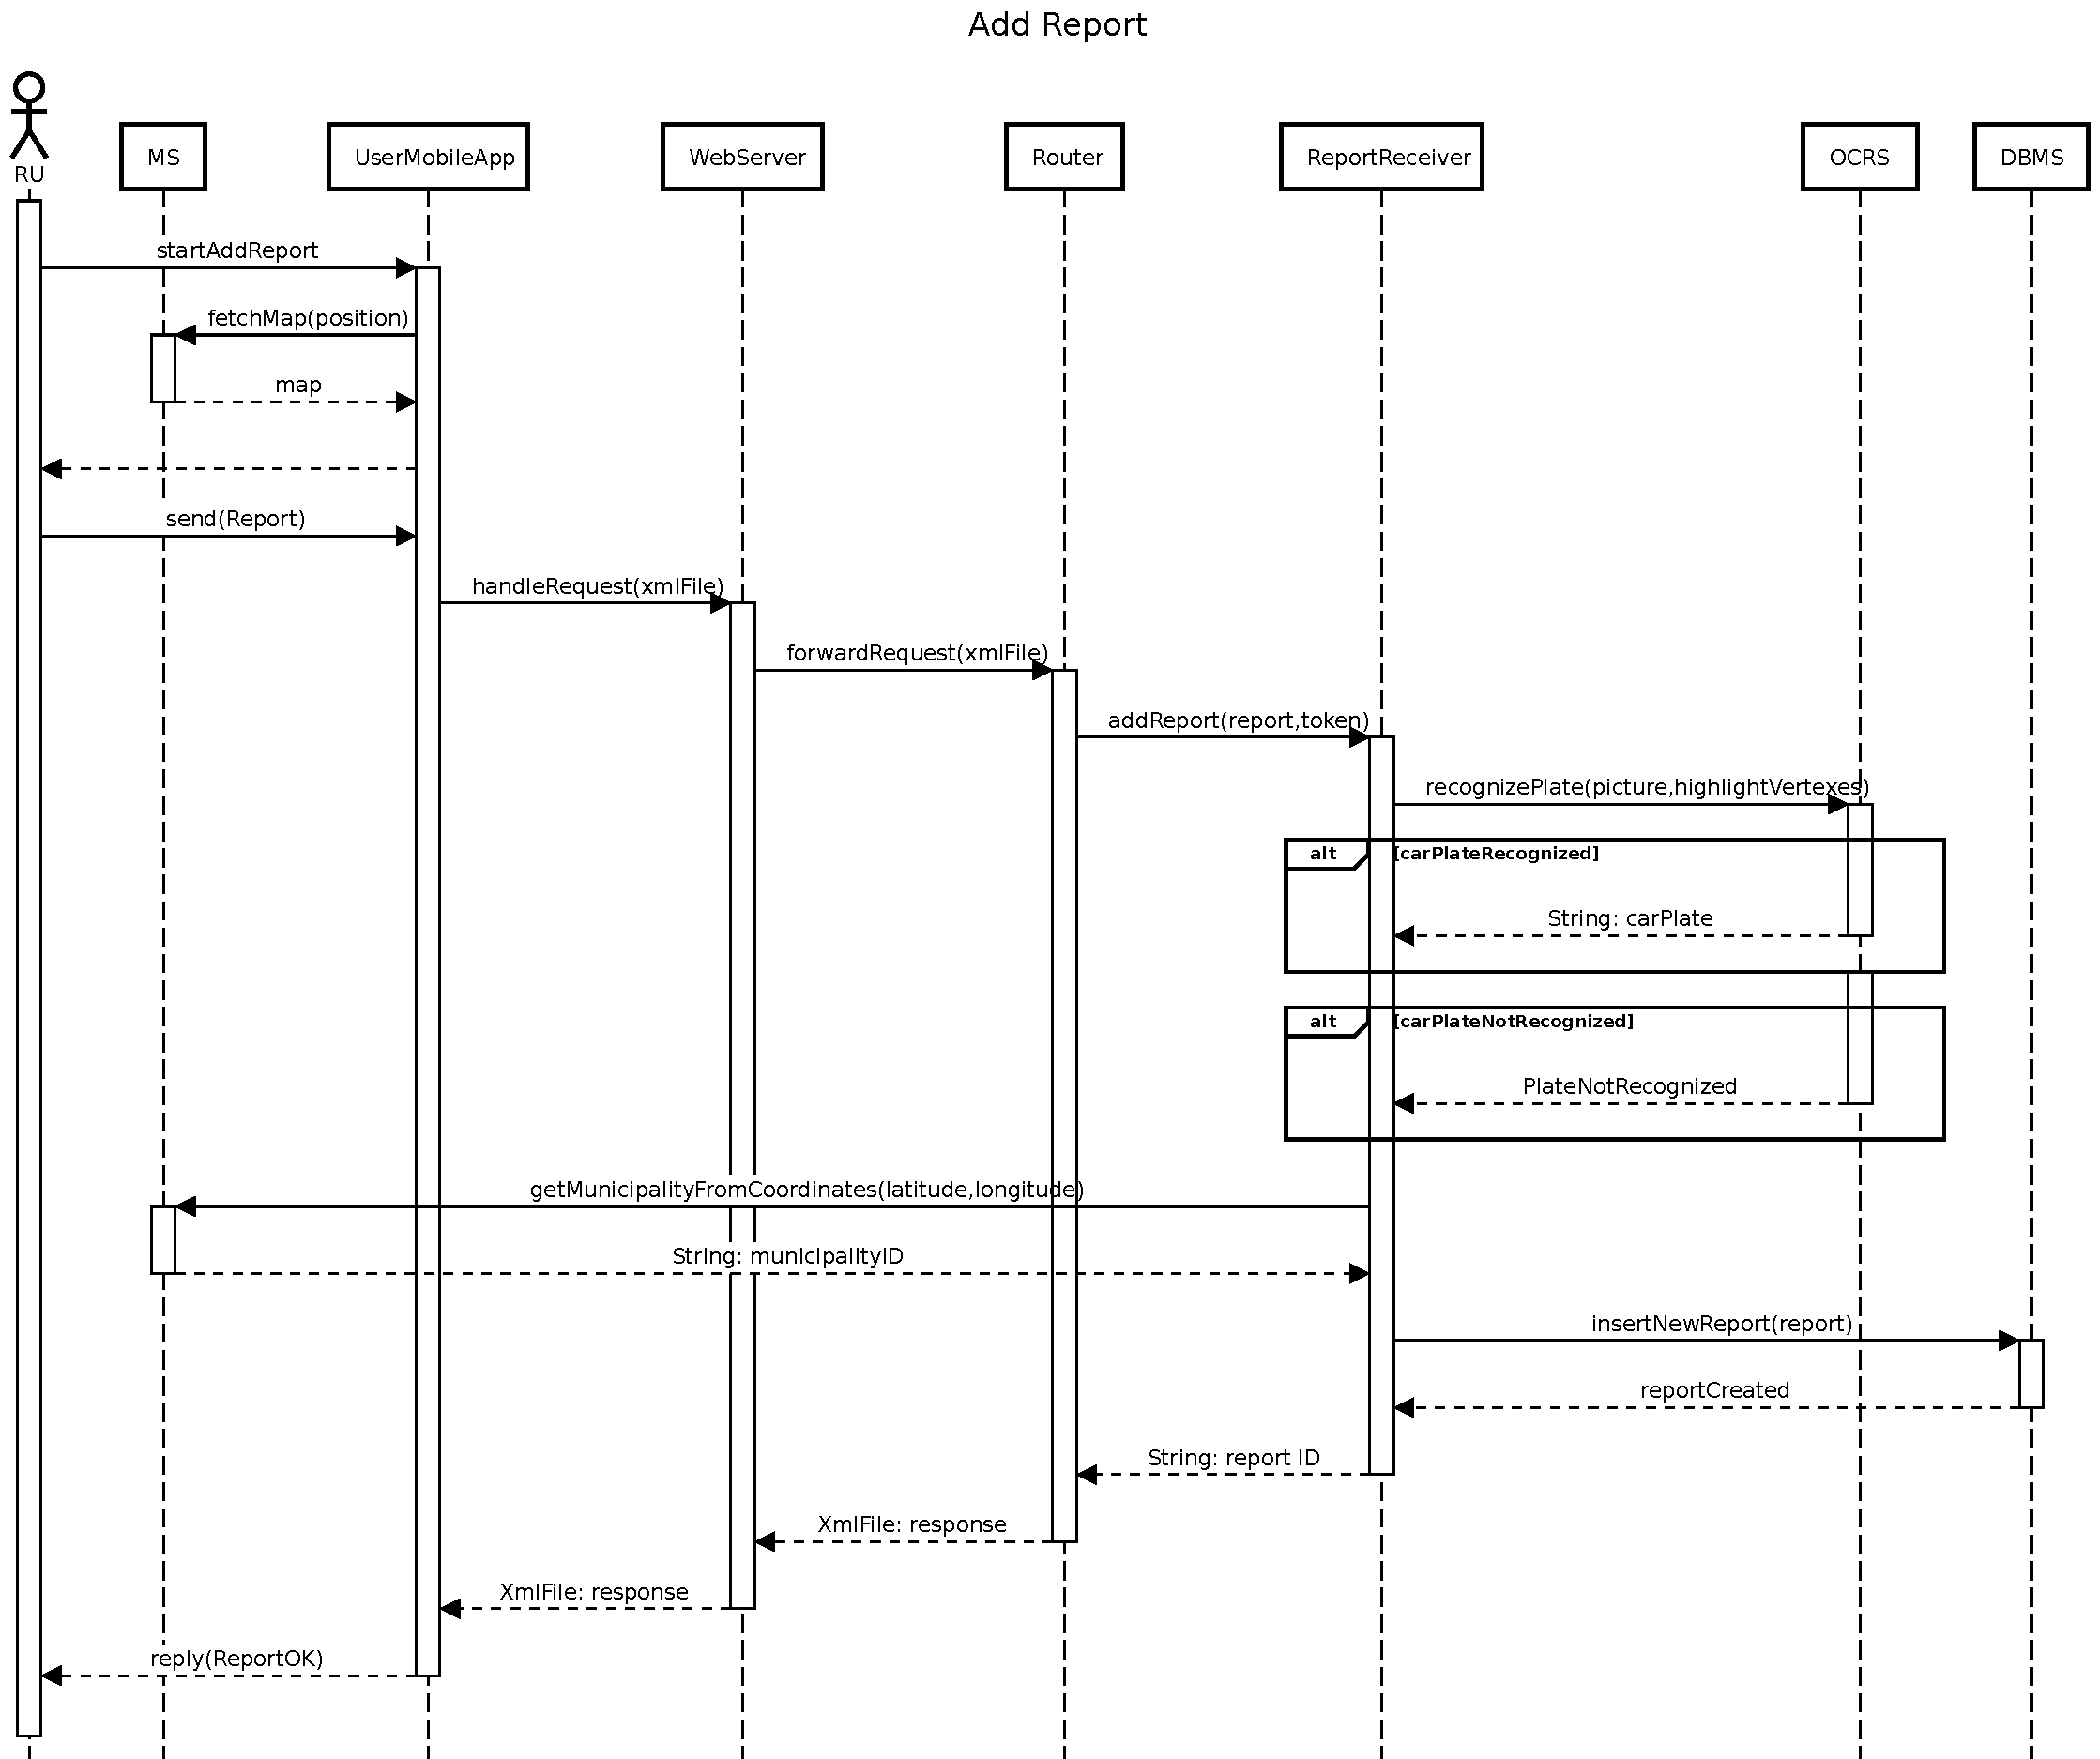
\includegraphics[width=\textwidth]{images/DD2/RuntimeView/RU/AddReport.pdf}
						\caption{Add report runtime view diagram}
					\end{figure}
					\paragraph{}
						In this sequence diagram the process through which a RU adds a report to the system is shown. 
						
						At first the RU chooses the "Add report" functionality on the UserMobileApp and composes the report. The app fetches a map from the MS and forwards the request to the Web Server, which contacts the Router. The Router forwards the request to the ReportReceiver, which tries to recognize the plate with the help of the OCRS, gets the municipality where the report has been issued through the MS and, finally, adds the report to the database through the QueryManager.
				\subsubsection{Get my reports}
					\begin{figure}[!h]
						\centering
						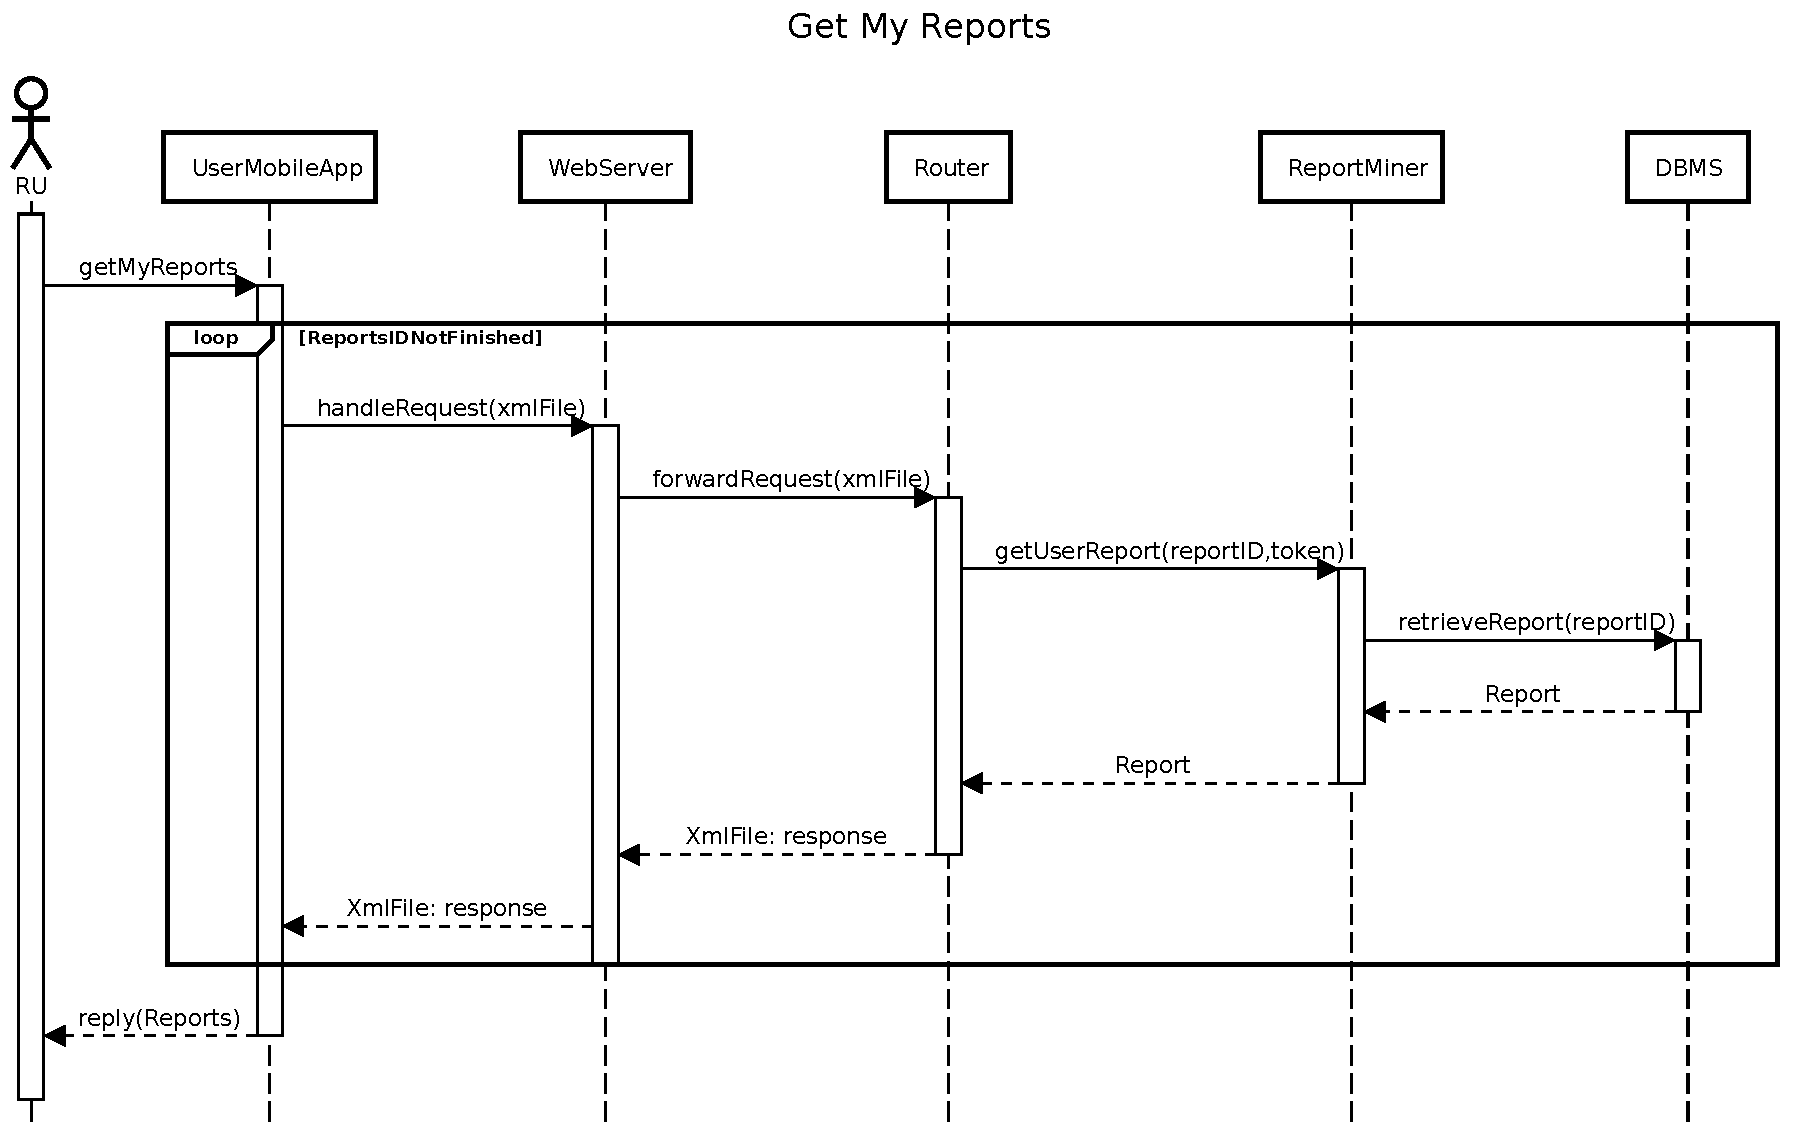
\includegraphics[width=\textwidth]{images/DD2/RuntimeView/RU/GetMyReports.pdf}
						\caption{Get my reports runtime view diagram}
					\end{figure}
					\paragraph{}
						In this sequence diagram the process through which a RU gets all the reports he/she has issued is shown.
						
						At first the RU chooses the "Get my reports" functionality on the UserMobileApp. Then the app starts fetching all the reports issued by the user. In particular, every request passes through the WebServer, Router, ReportMiner and finally the QueryManager, then it goes back to the UserMobileApp. Once all the reports have been fetched, they are presented to the RU.
				\clearpage
				\subsubsection{Get unsafe areas}
					\begin{figure}[!h]
						\centering
						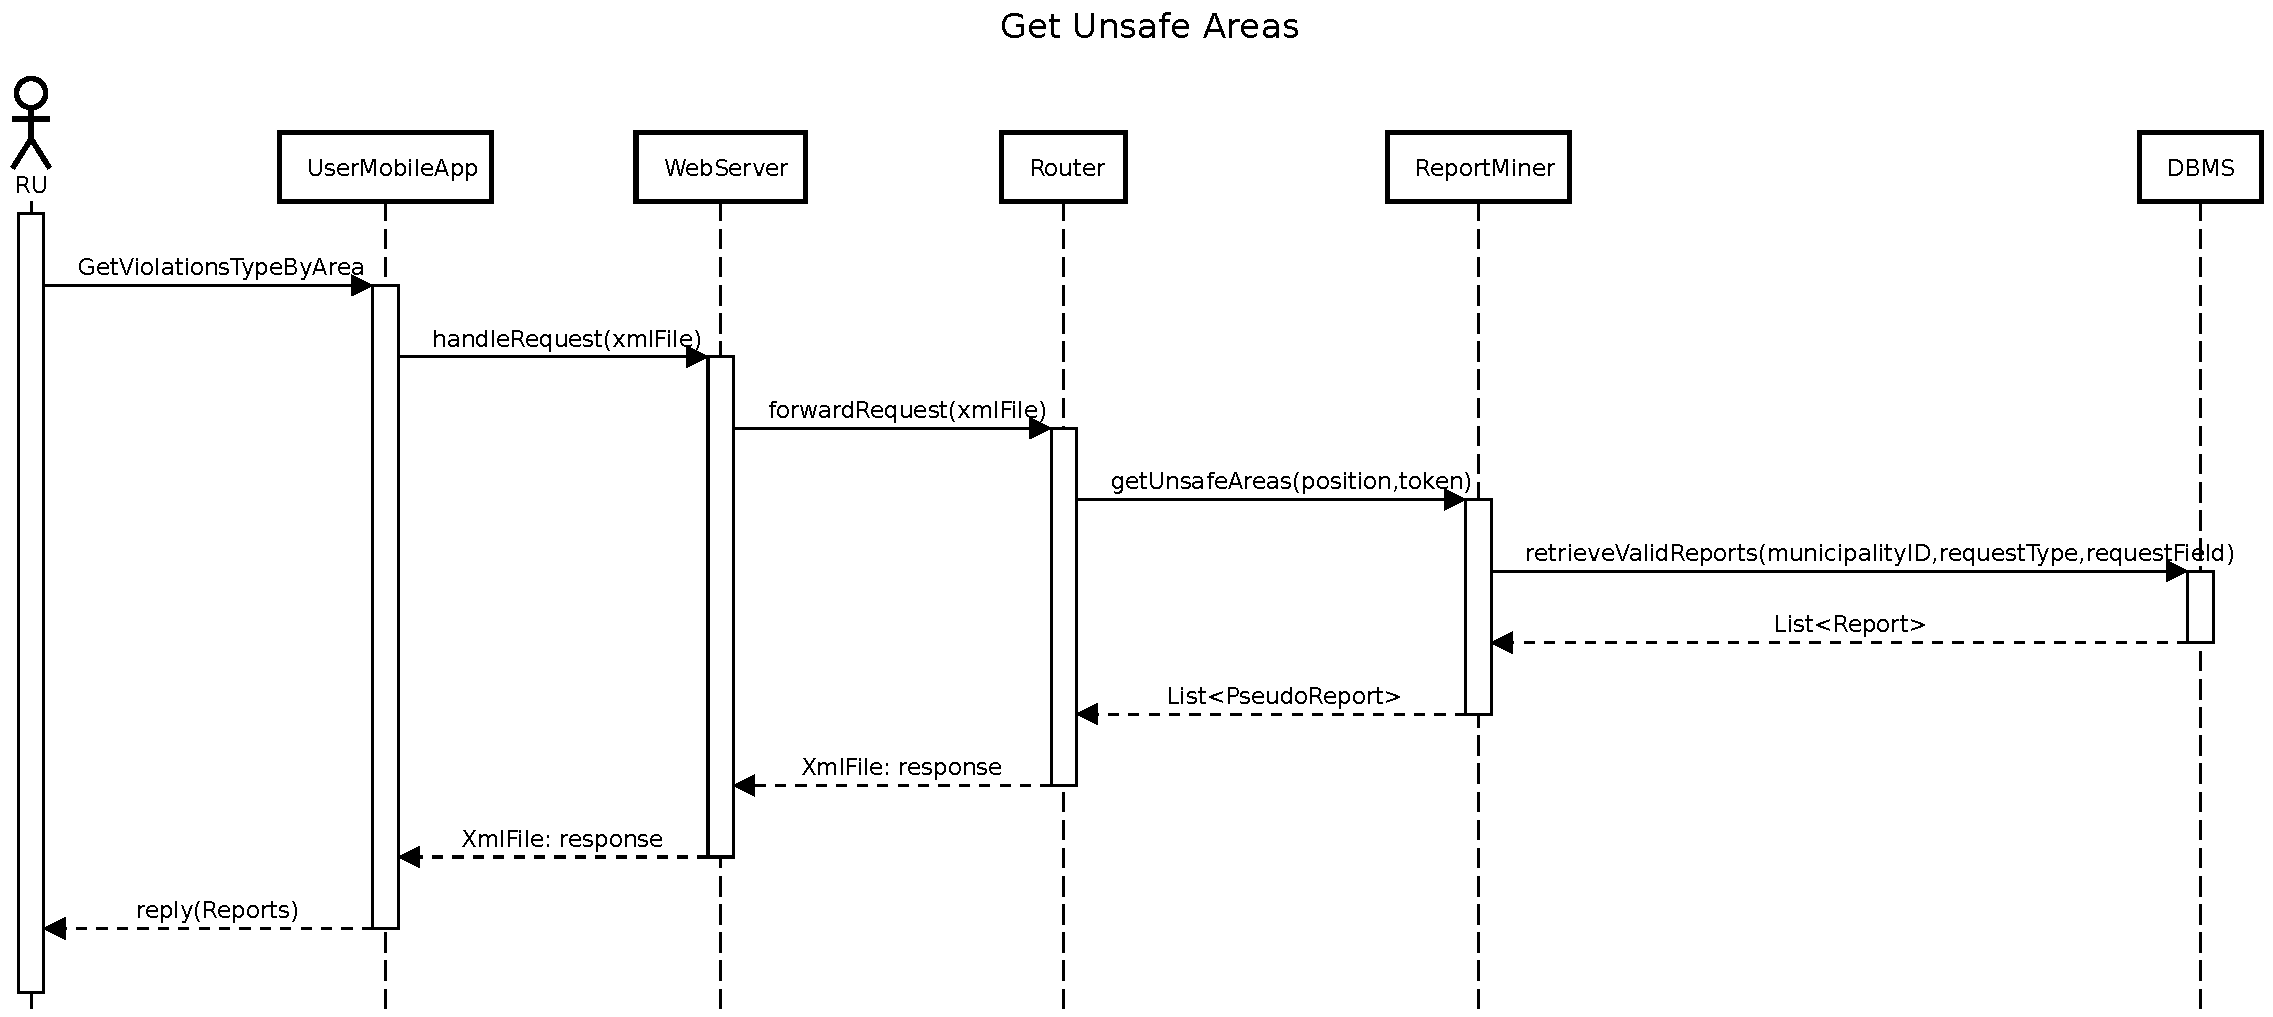
\includegraphics[width=\textwidth]{images/DD2/RuntimeView/RU/GetUnsafeAreas.pdf}
						\caption{Get unsafe areas runtime view diagram}
					\end{figure}
					\paragraph{}
						In this sequence diagram is displayed the process which permits a RU to discover all the types, dates and times of reports issued in a selected area. 
						
						This starts with the request, by the RU, that gets sent to the Web Server which will forward it to the Router. The Router will call "getUnsafeAreas" on the ReportMiner component that will query the database, through the QueryManager. When the response is ready it will go back through the same path.
			\clearpage
			\subsection{Authority}
				\subsubsection{Get statistics}
					\begin{figure}[!h]
						\centering
						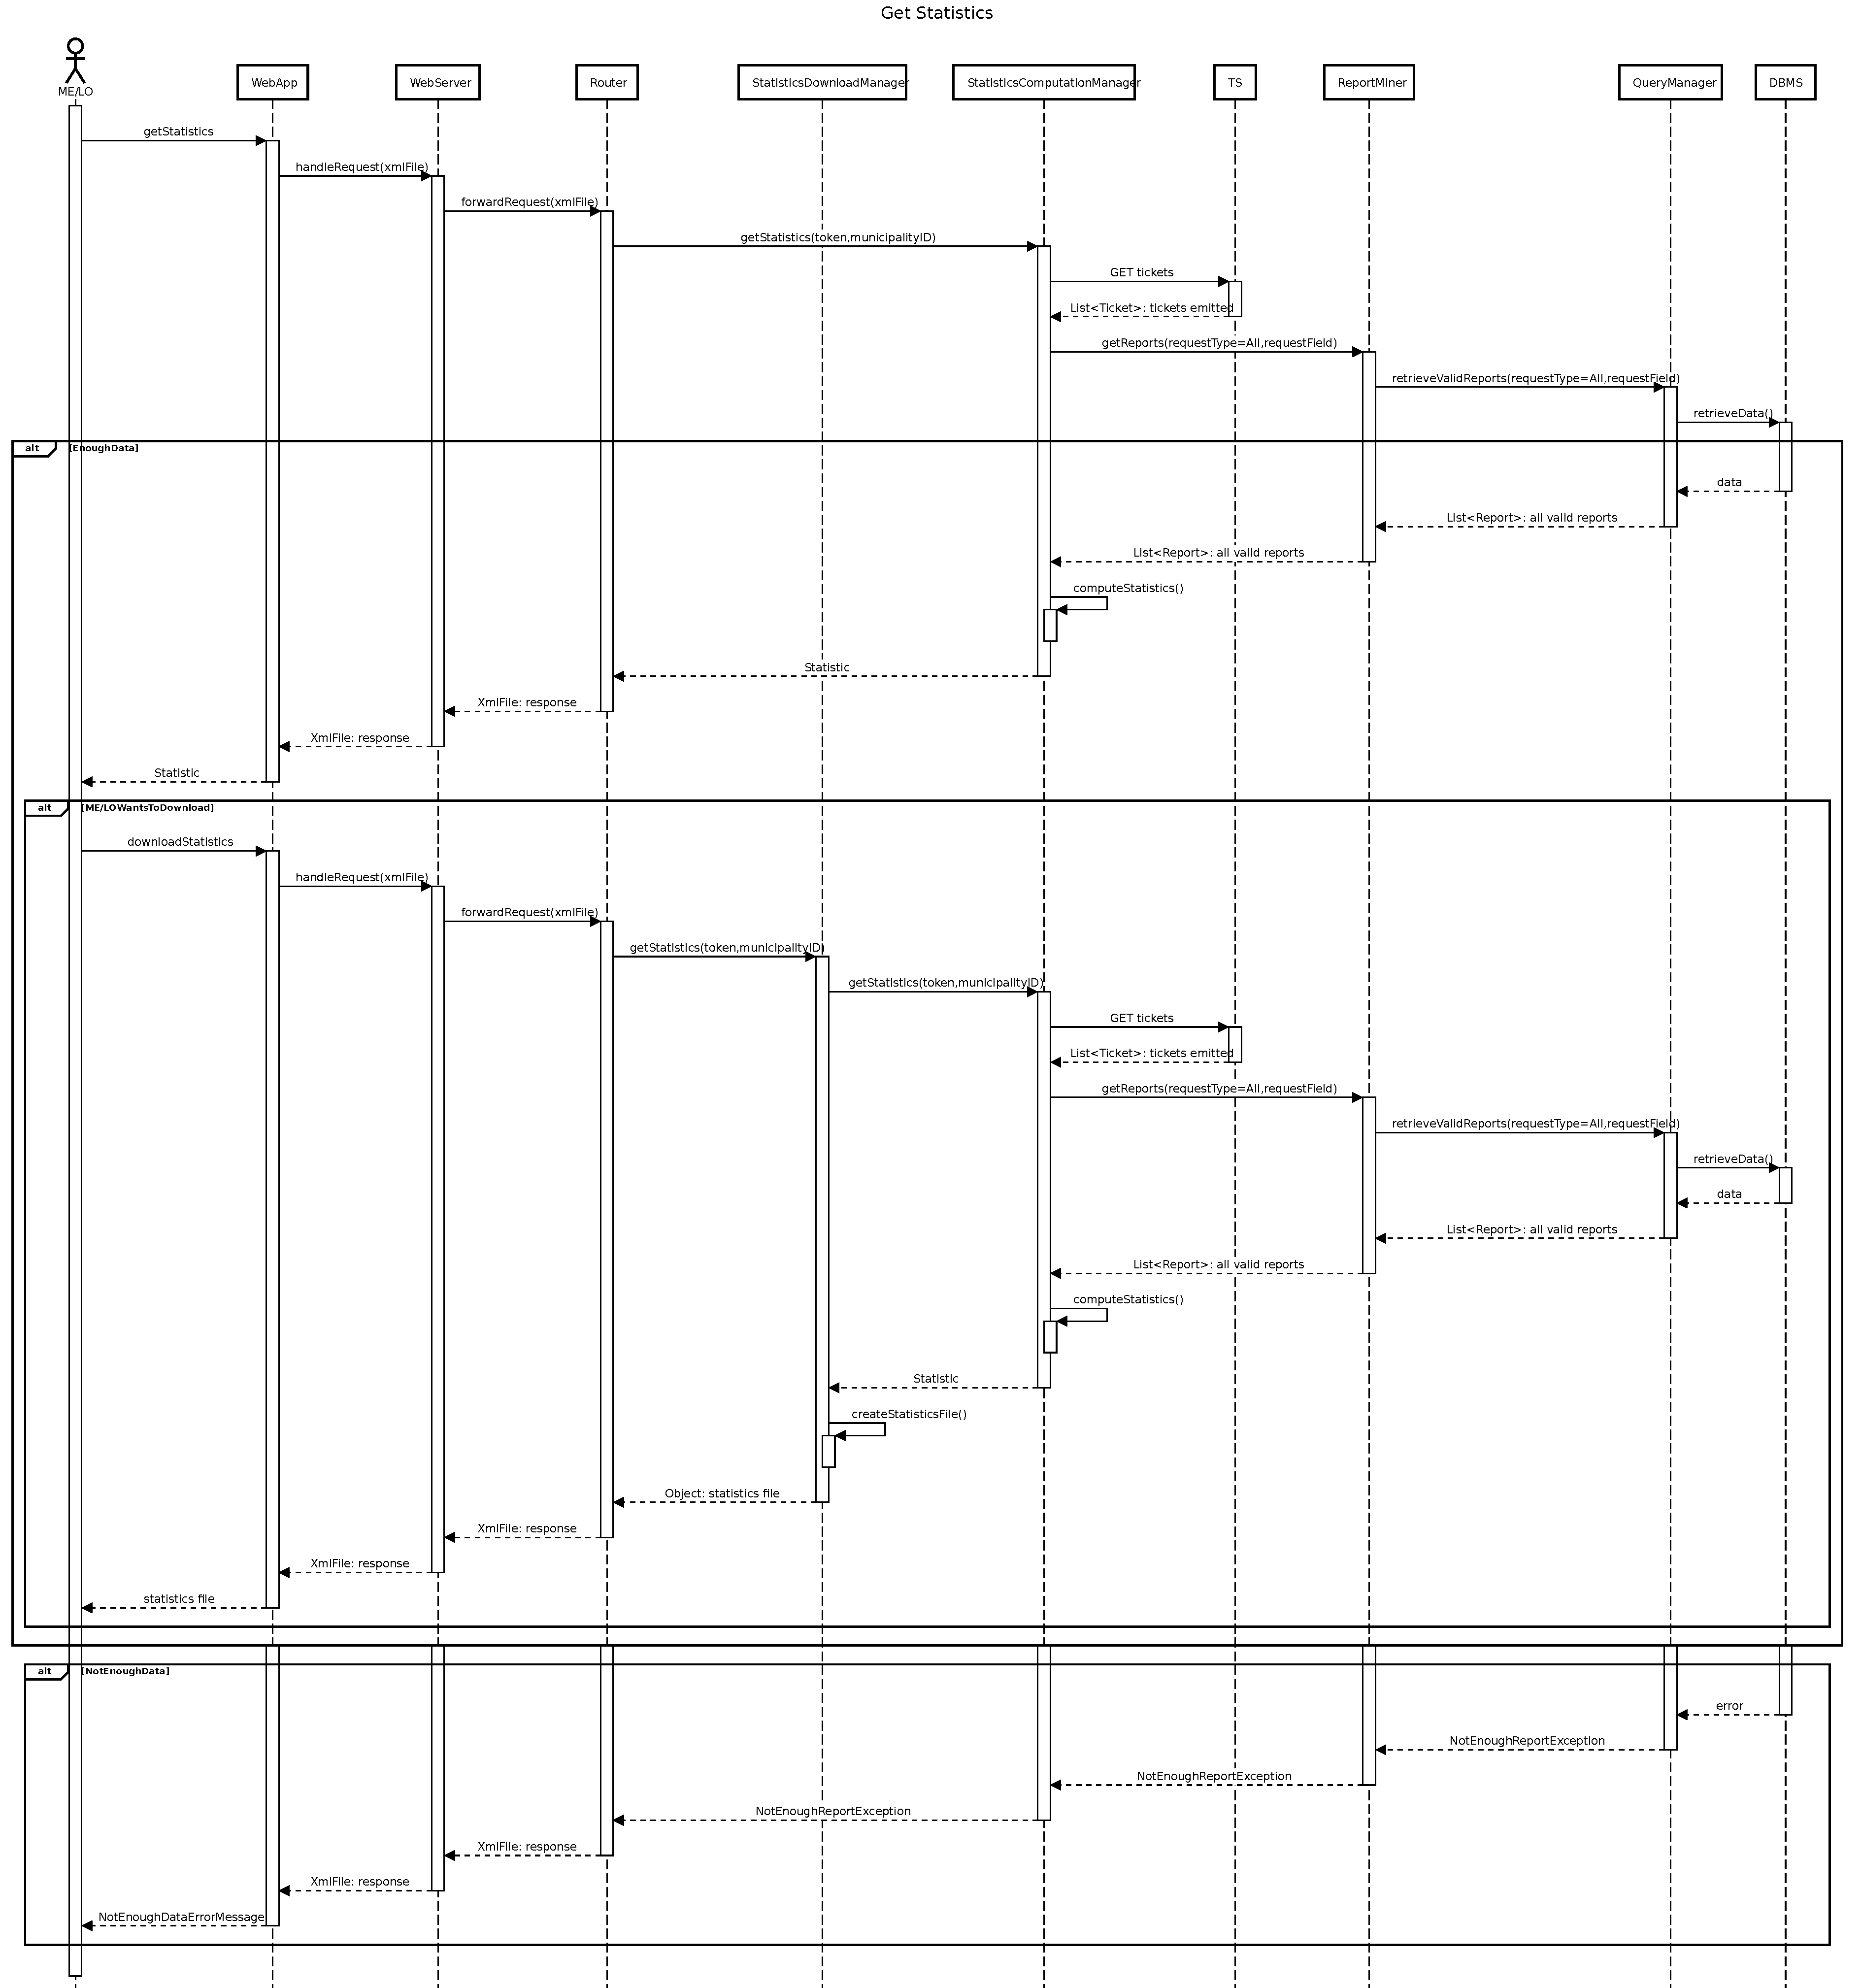
\includegraphics[width=\textwidth]{images/DD2/RuntimeView/Authority/GetStatistics.pdf}
						\caption{Get statistics runtime view diagram}
					\end{figure}
					\paragraph{}
						In this sequence diagram the request gets sent to the WebServer and forwarded to the Router. Here, the StatisticsComputationManager is called. This component requests tickets data from the TS and then uses the ReportMiner component to get reports, through the QueryManager. If there are enough data, the StatisticsComputationManager generates new statistics. If the request from the authority was to only visualize the statistics, the StaticsComputationManager will send them back to the Router and to the authority, otherwise, by starting a new request, the StatisticsDownloadManager asks the StaticsComputationManager for new statistics, creates a non{-}materalized document and sends it back through the Router.
				\clearpage
				\subsubsection{Mine reports}
					\begin{figure}[!h]
						\centering
						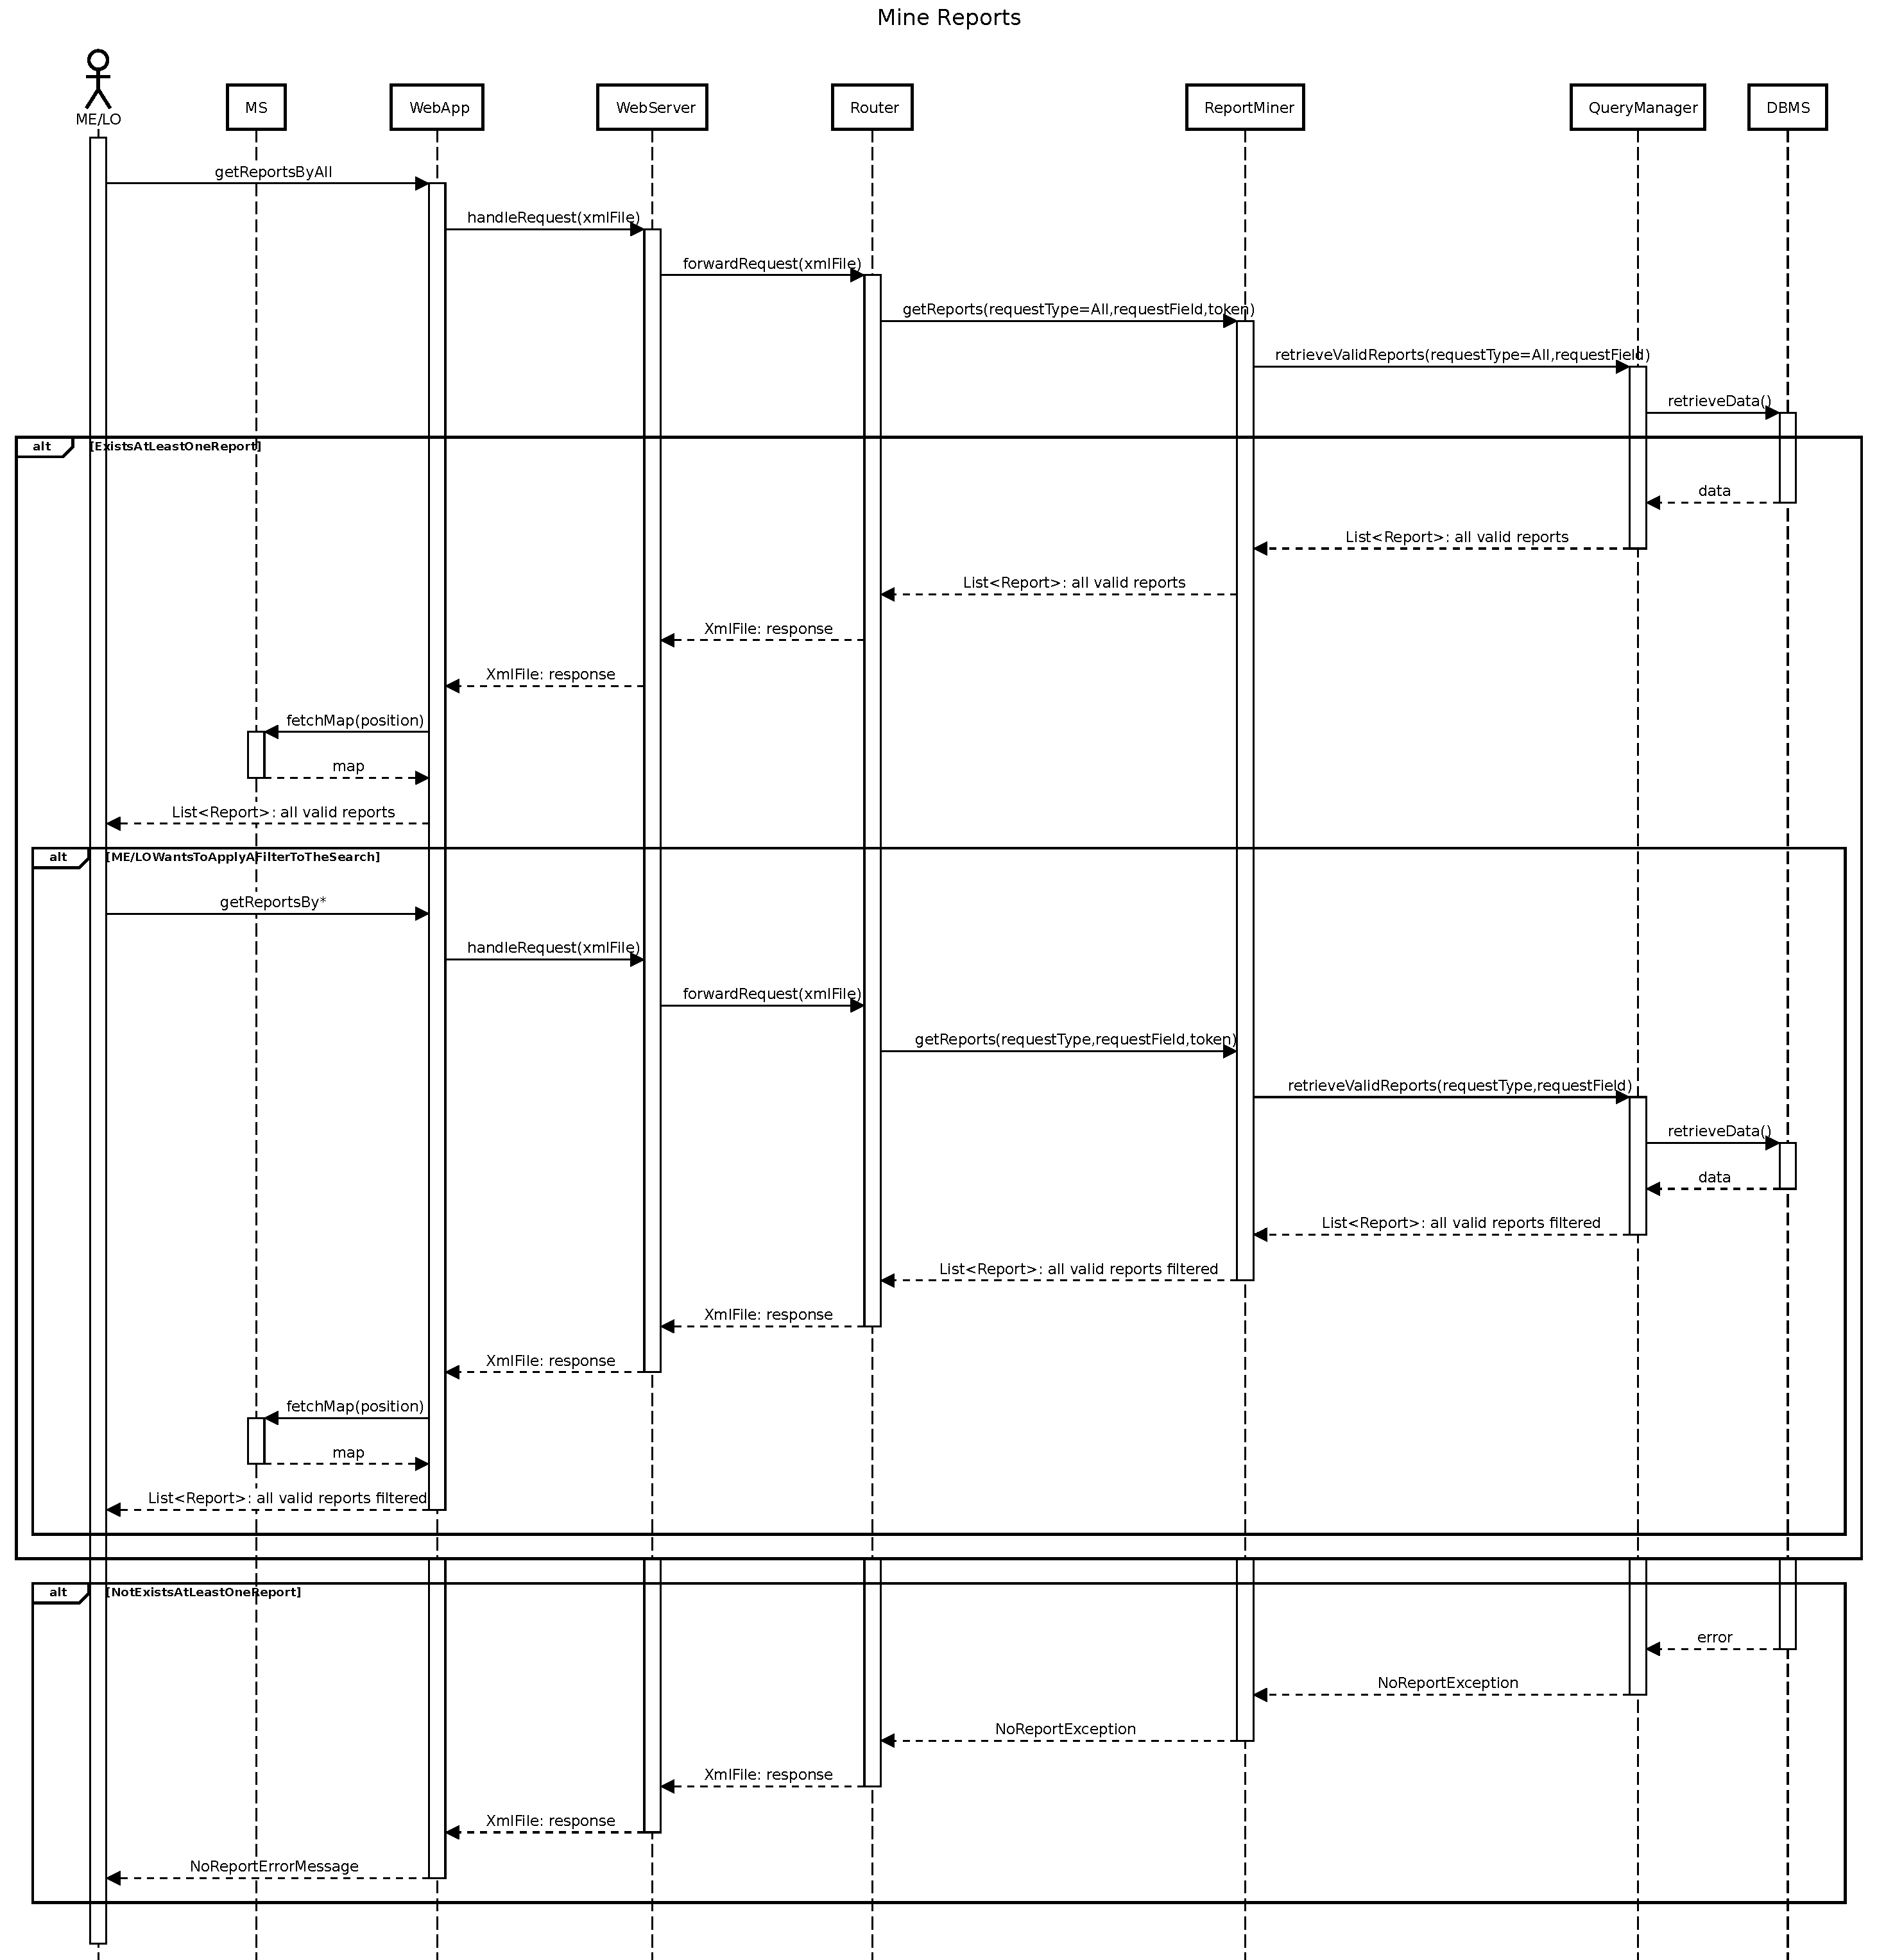
\includegraphics[width=\textwidth]{images/DD2/RuntimeView/Authority/MineReports.pdf}
						\caption{Mine reports runtime view diagram}
					\end{figure}
					\paragraph{}
						This sequence diagram shows how the authorities can mine the reports. 
						
						At first all the reports in the authority's municipality are fetched through the following procedure. The mine request gets sent from the Web App to the Web Server which sends it forward to the Router. The ReportMiner gets called, it queries the database, through the QueryManager, and, if enough reports are found, the list containing them is created and sent back to Web App. When there are less reports than needed, an error message will reach the authority. When the Web App receives the list of reports, it uses the MS to display them. 
						
						Now the requester is able to decide a filter to the search, choosing between the ones described in the ReportMiner component description. In order to fetch the filtered reports, the same procedure described before is used, but the requestType will be different from "ALL".
			\clearpage
			\subsection{Local Officer}
				\subsubsection{Validate reports}
					\begin{figure}[!h]
						\centering
						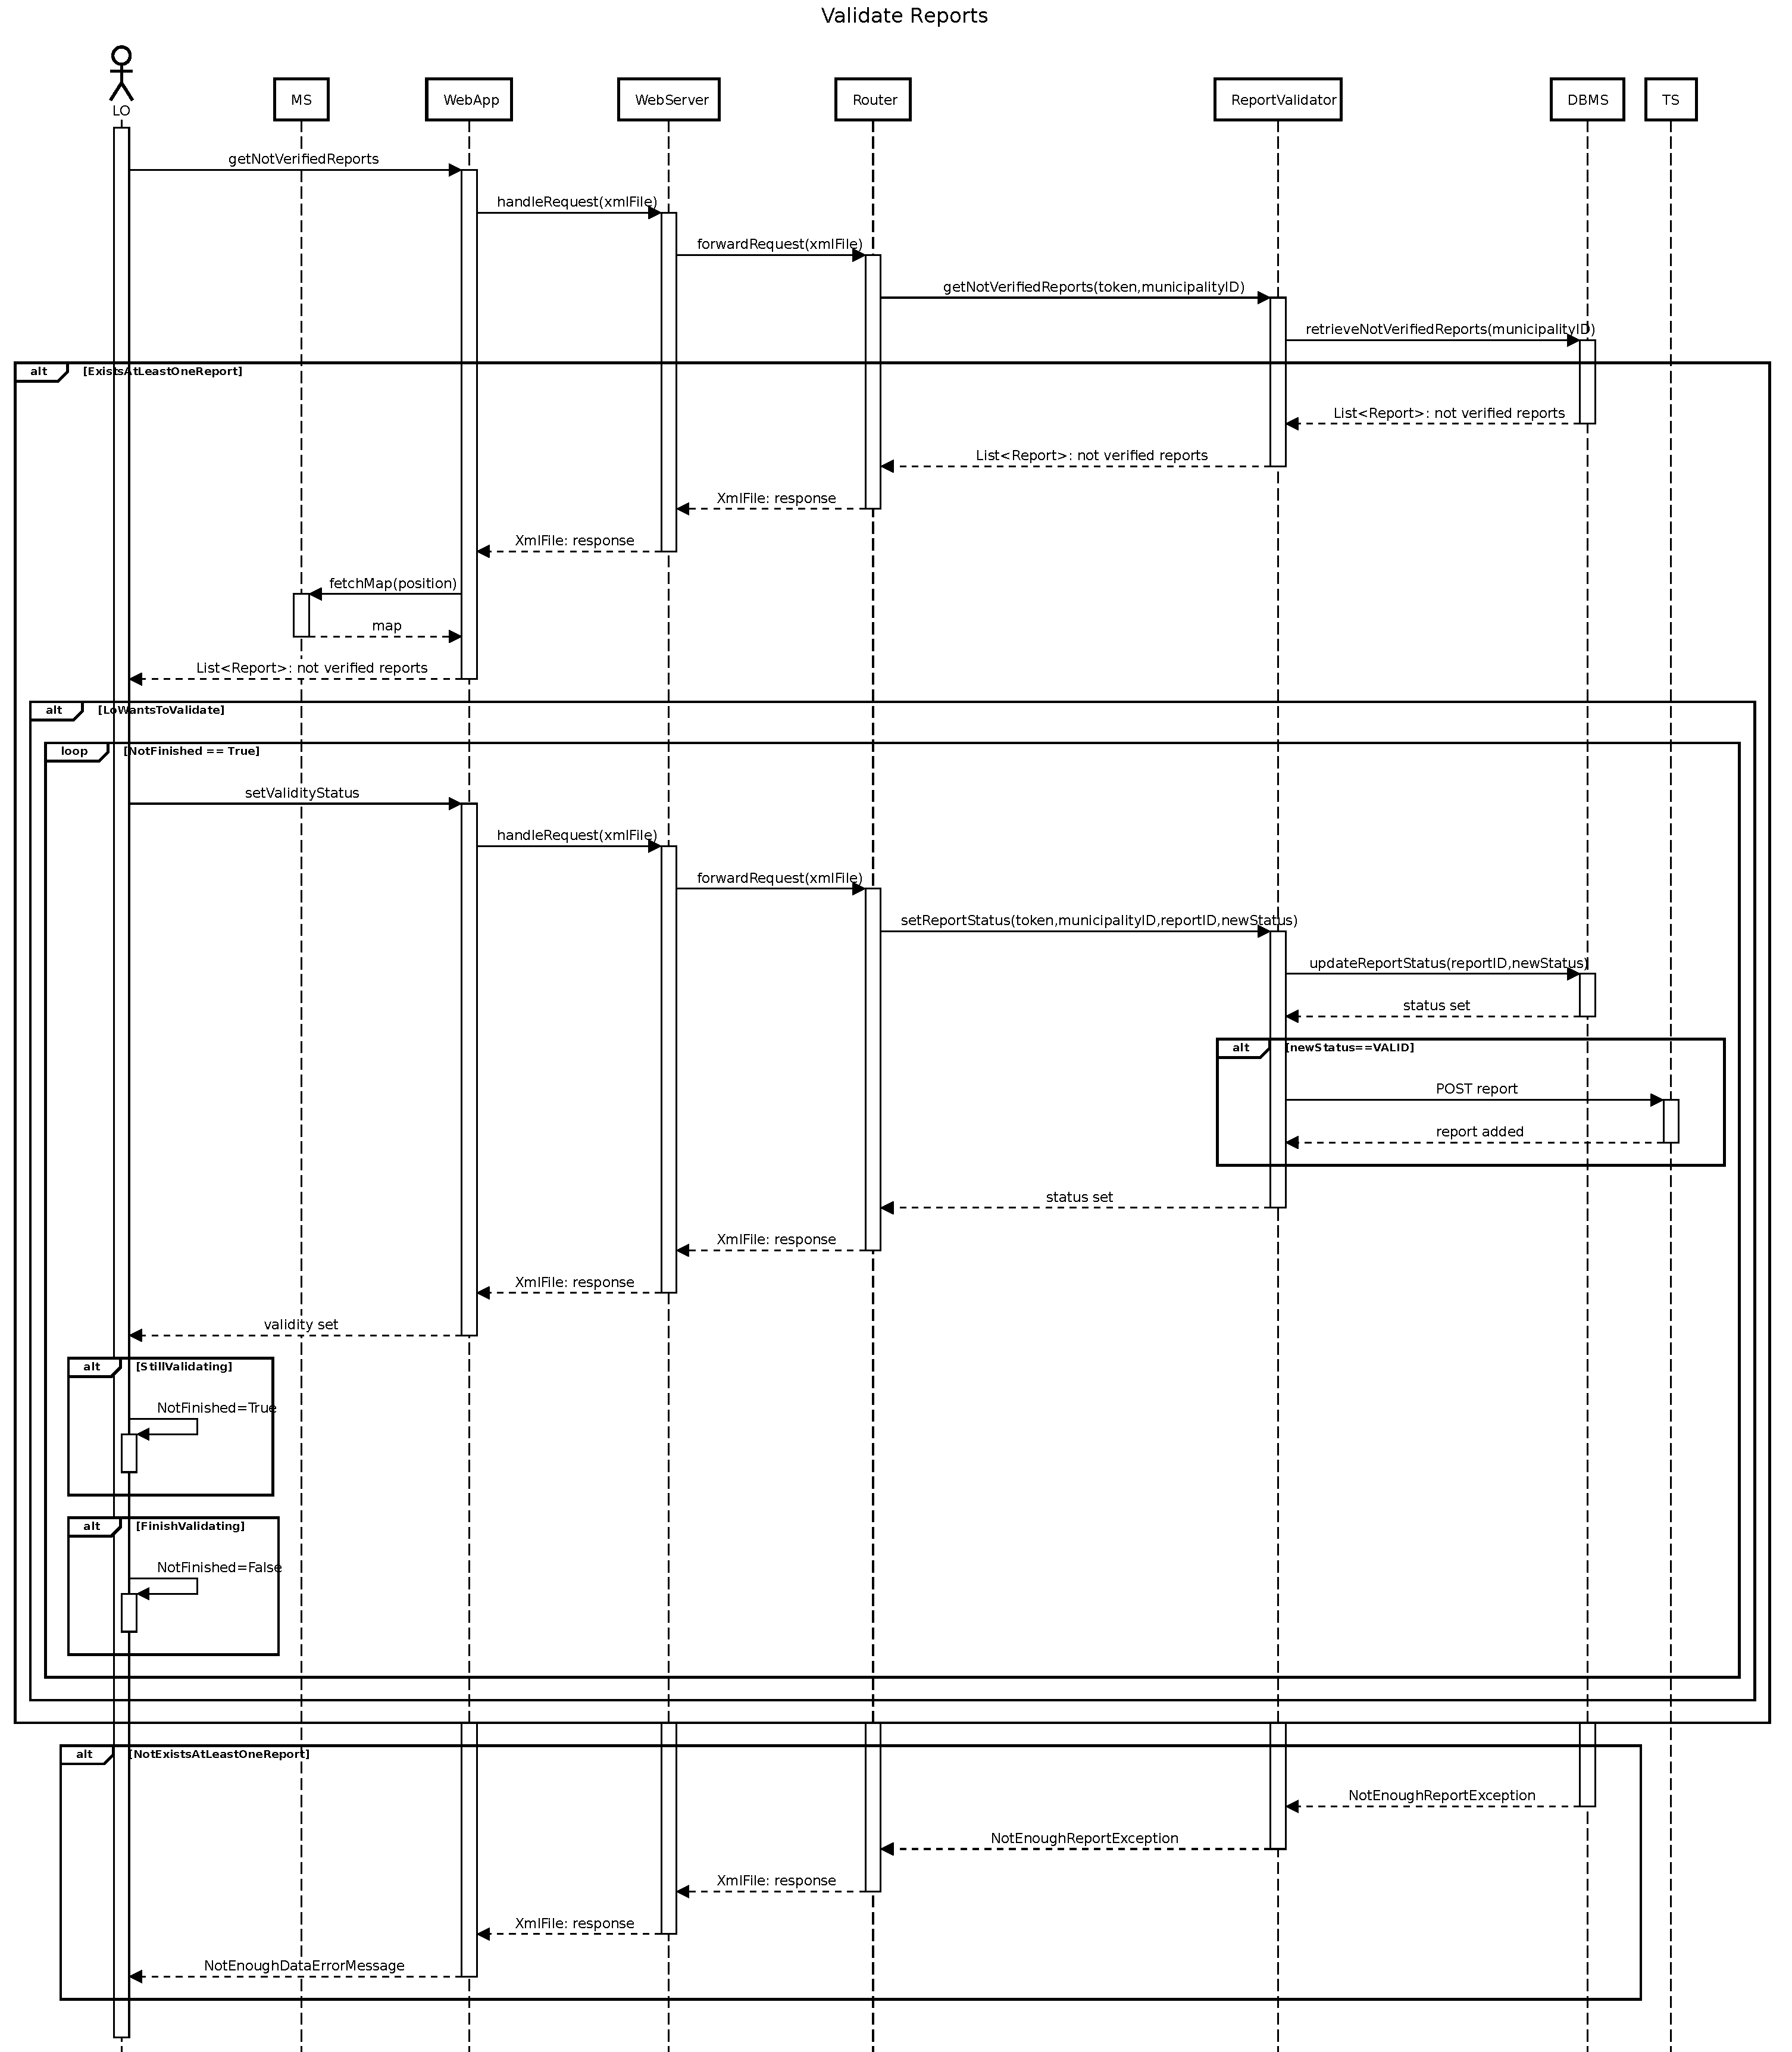
\includegraphics[width=\textwidth]{images/DD2/RuntimeView/Authority/LO/ValidateReports.pdf}
						\caption{Validate reports runtime view diagram}
					\end{figure}
					\paragraph{}
						The request gets sent with the standard route until the ReportValidator gets reached. ReportValidator queries the QueryManager for reports to be validated, if there are none an error message is shown back to the Web App, otherwise the reports are sent back to the Web App, where they are displayed also thanks to the MS.
						The LO can at this point start to validate the reports. When a report gets validated, with any result of validation, it gets sent back to the ReportValidator component which updates the database, through the QueryManager, and, if the report is set as "VALID", it is also sent to the TS with a POST request. The process continues until the LO stops to validate reports.
			\clearpage
			\subsection{Municipal Employee}
				\subsubsection{Get improvements}
					\begin{figure}[!h]
						\centering
						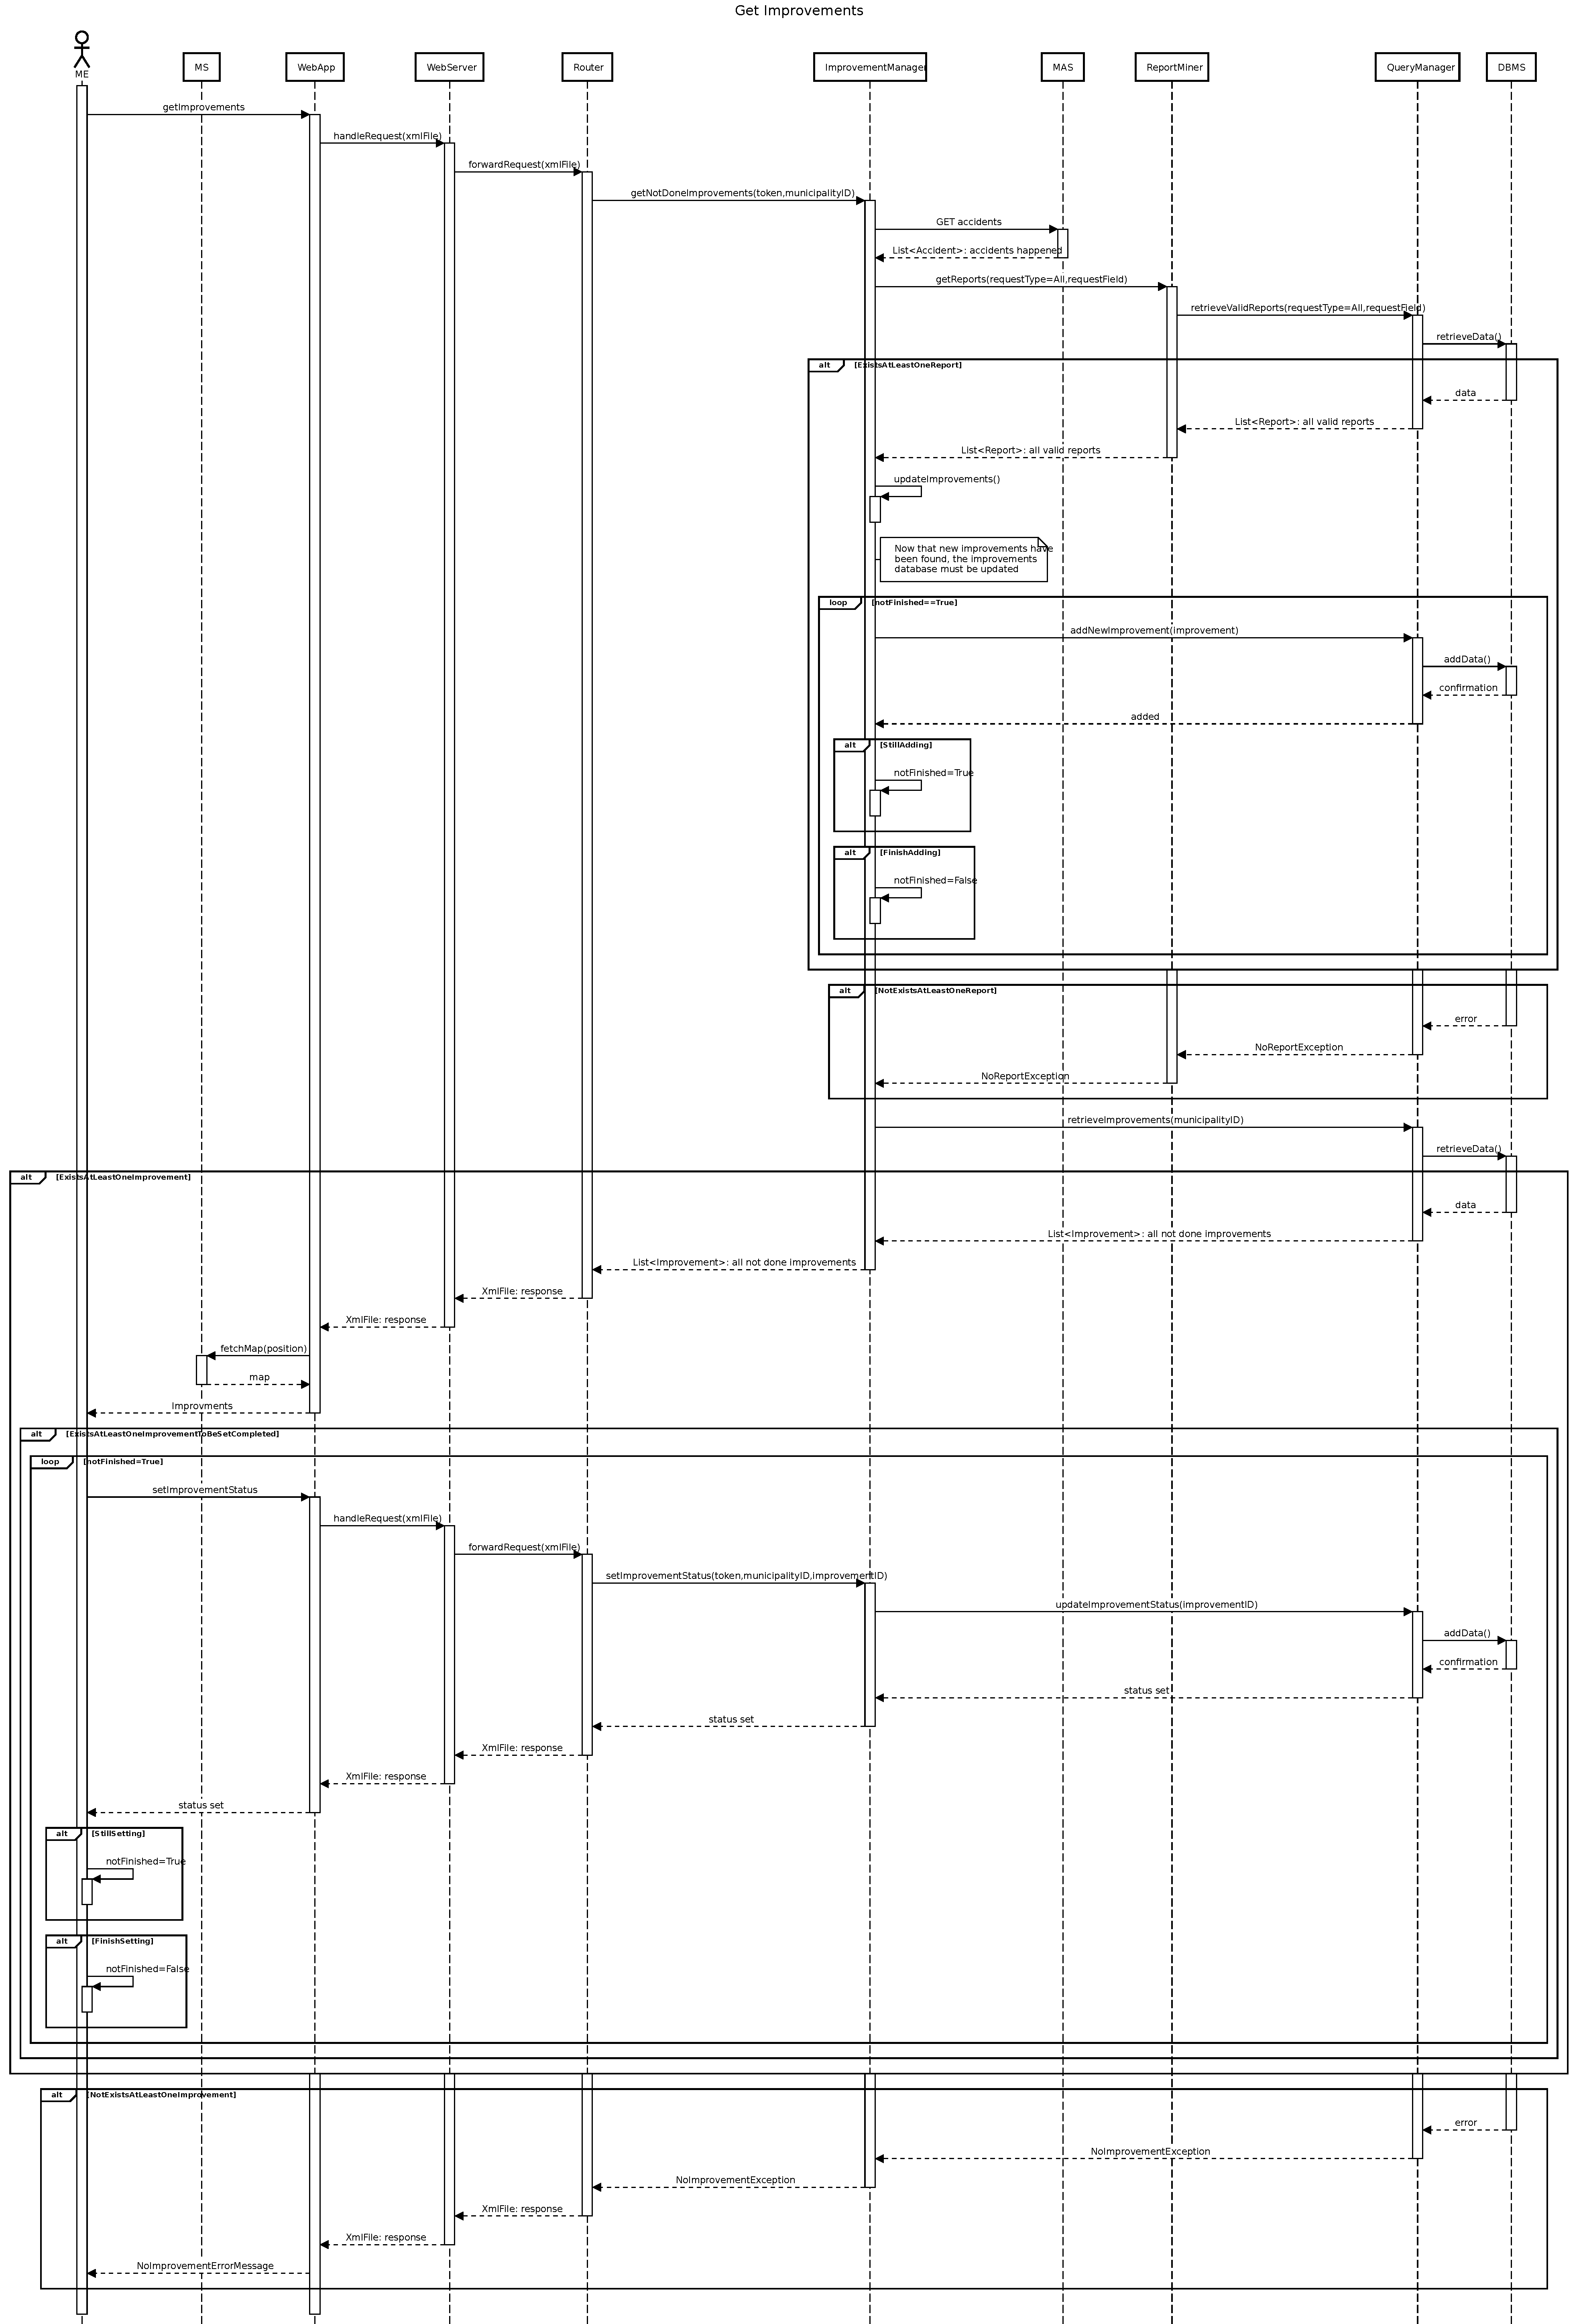
\includegraphics[width=\textwidth]{images/DD2/RuntimeView/Authority/ME/GetImprovements.pdf}
						\caption{Get improvements runtime view diagram}
					\end{figure}
					\paragraph{}
						This sequence diagram shows the request of improvements from a ME. 
						
						Using the standard route, the request reaches the ImprovementManager, which gets from the MAS, through a GET request, the list of accidents that took place in the ME's municipality. The ReportMiner then is tasked to obtain, from the QueryManager, the list of reports of the municipality, retuning them in case of success, or returning an error to the Web App in case of failure. 
						
						With the data received from the MAS and the ReportMiner, the ImprovementManager computes all possible improvements that, in a loop, are sent and memorized on the database only if they were not already present. Finished the update, the ImprovementManager retrieves from the database, using the "retrieveImprovements" function of the QueryManager, all possible "NOT DONE" improvements for the ME's municipality. The list of improvements is then sent back through the Router to the Web App where the ME can visualize and eventually set them as "DONE". 
						
						When at least one improvement gets its status changed, the Web App sends a request back to the Web Server and the Router. The ImprovementManager is then called by the Router to update the status of the improvement on the database.
			\subsection{Extra cases}
				\subsubsection{Database access error}
					\begin{figure}[!h]
						\centering
						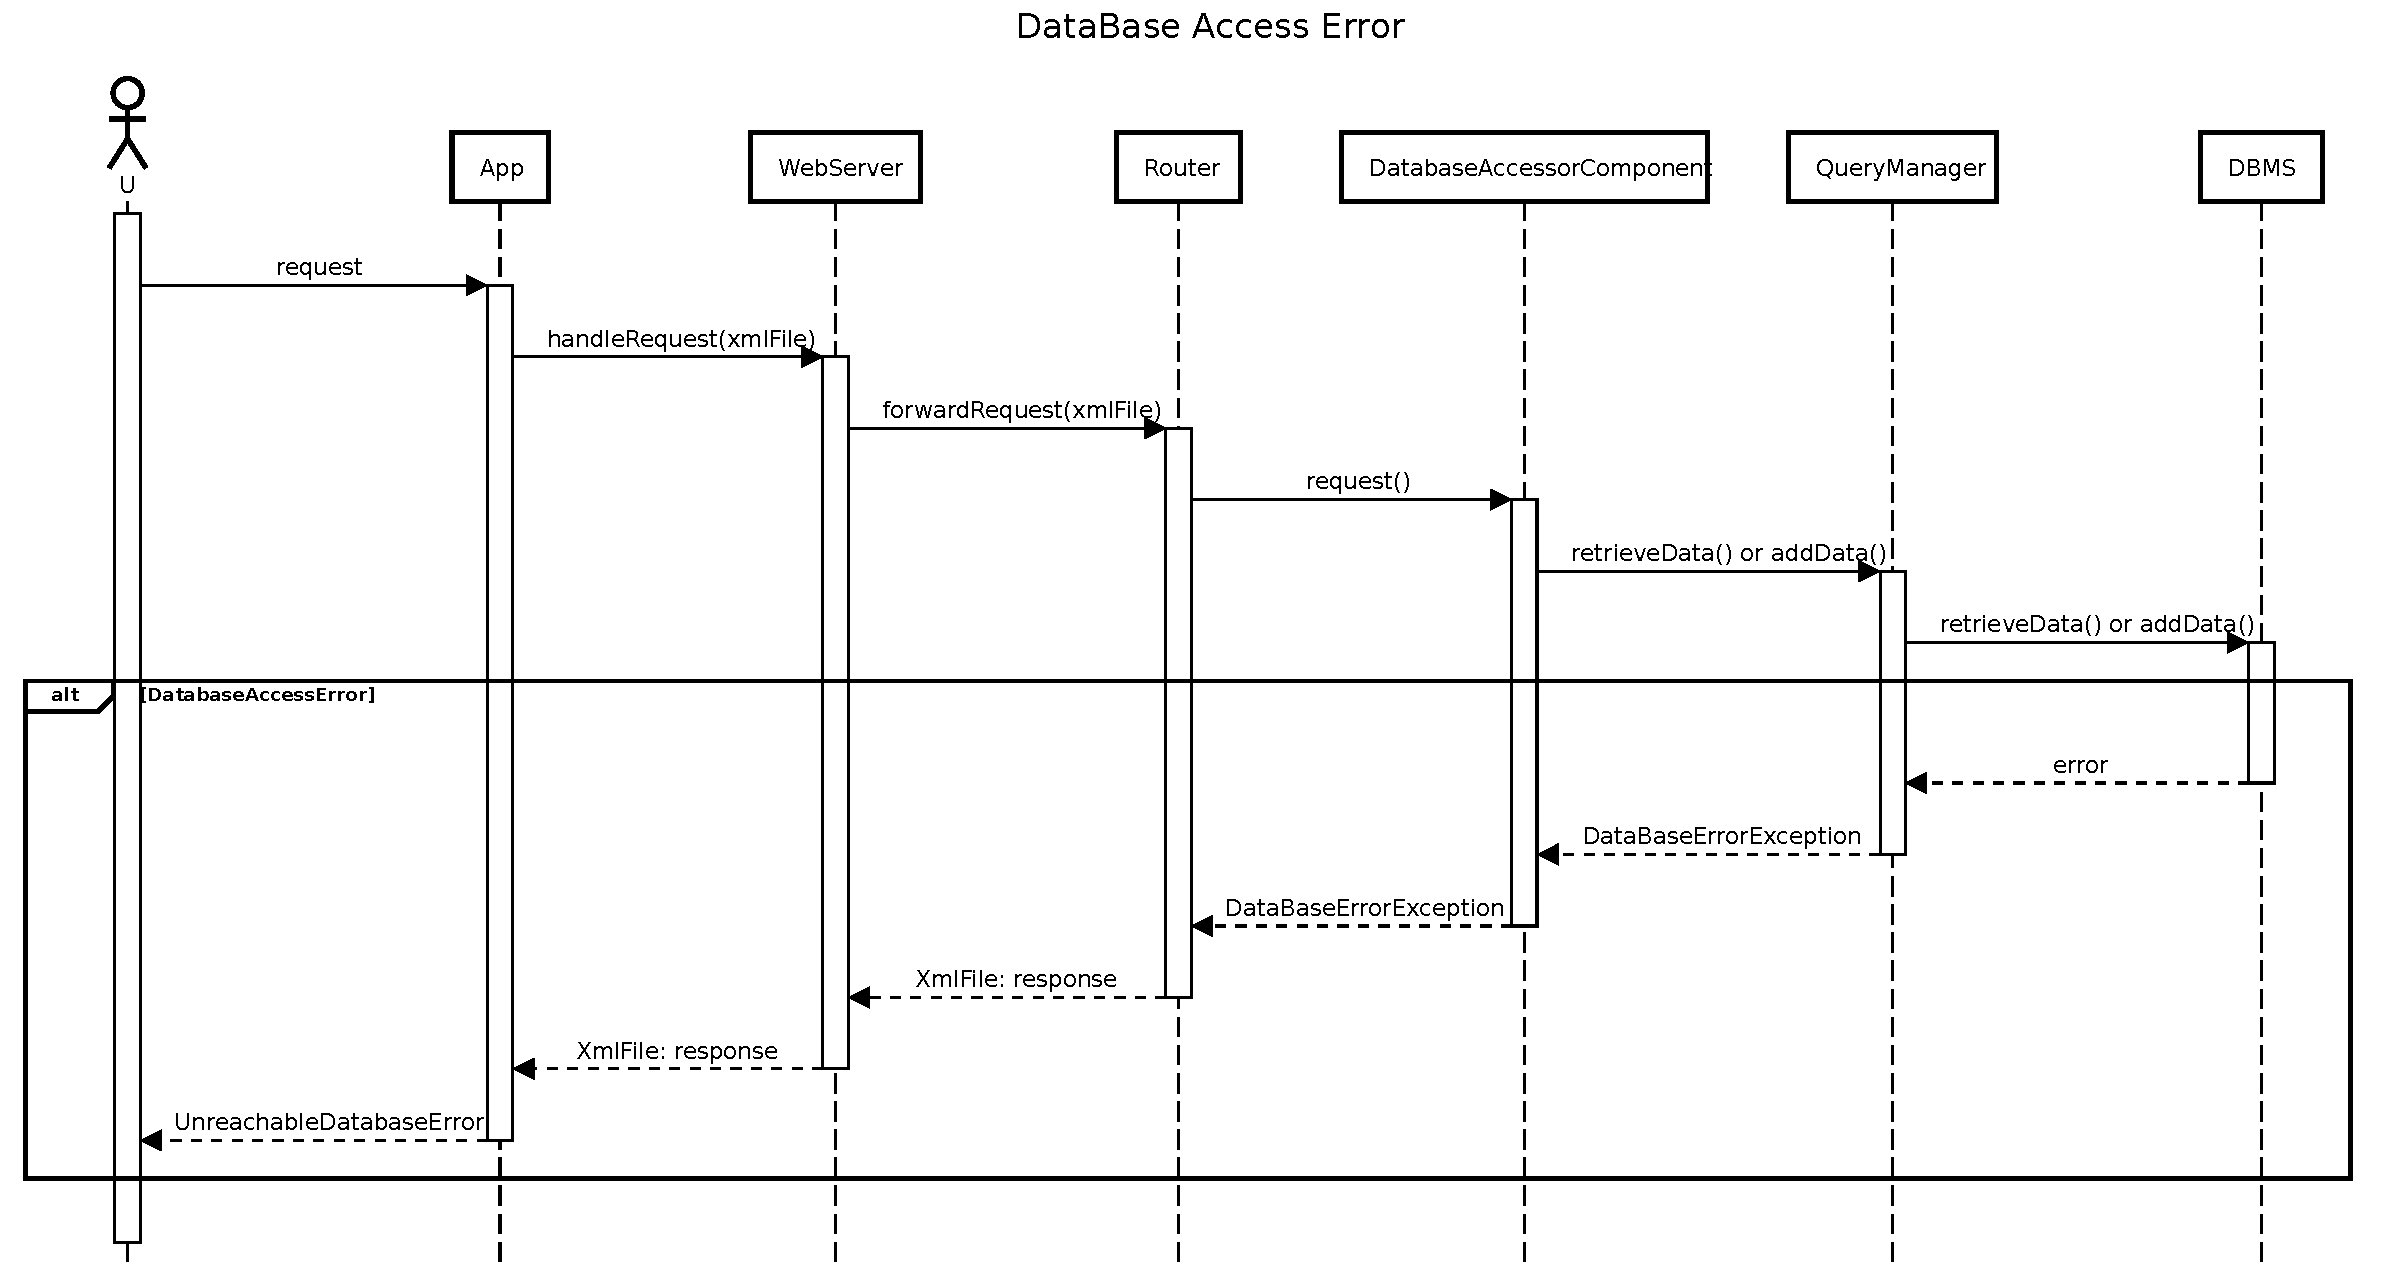
\includegraphics[width=\textwidth]{images/DD2/RuntimeView/Error/dbAccessError.pdf}
						\caption{Database access error runtime view diagram}
					\end{figure}
					\paragraph{}
						In this case a user U (which can be a RU, ME or LO) tries to use a functionality that accesses the database, but the database is not accessible.
				\clearpage
				\subsubsection{Invalid token}
					\begin{figure}[!h]
						\centering
						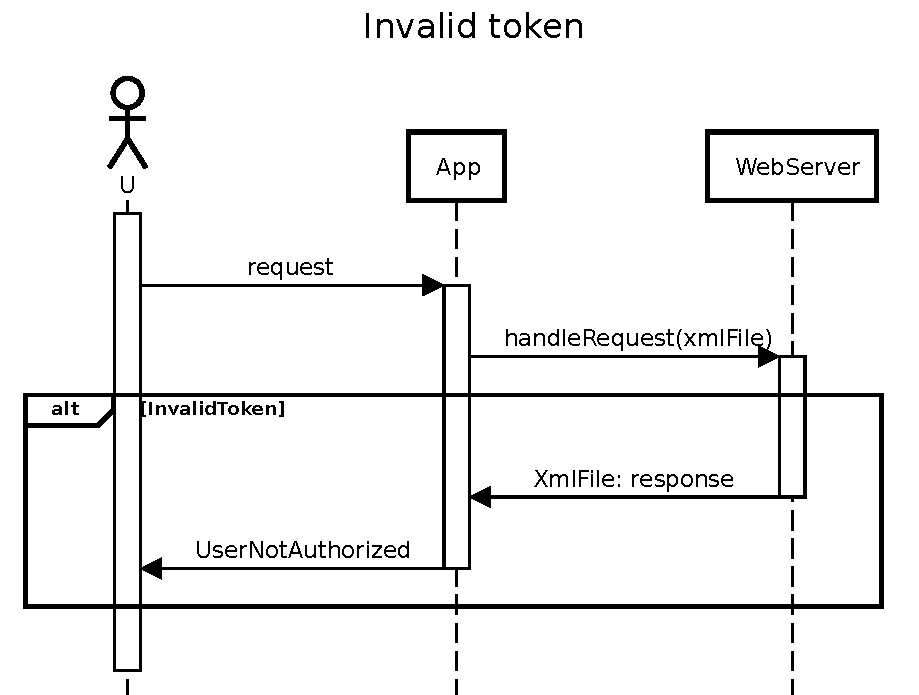
\includegraphics[width=0.6\textwidth]{images/DD2/RuntimeView/Error/invalidToken.pdf}
						\caption{Invalid token runtime view diagram}
					\end{figure}
					\paragraph{}
						In this case a user U (which can be a RU, ME or LO) tries to use a functionality that is not accessible with the given token (for example a RU that tries to MineReport).
		\section{Component interfaces}
			\paragraph{}
				The following picture contains all the used interface in the system.
				\begin{figure}[!h]
					\centering
					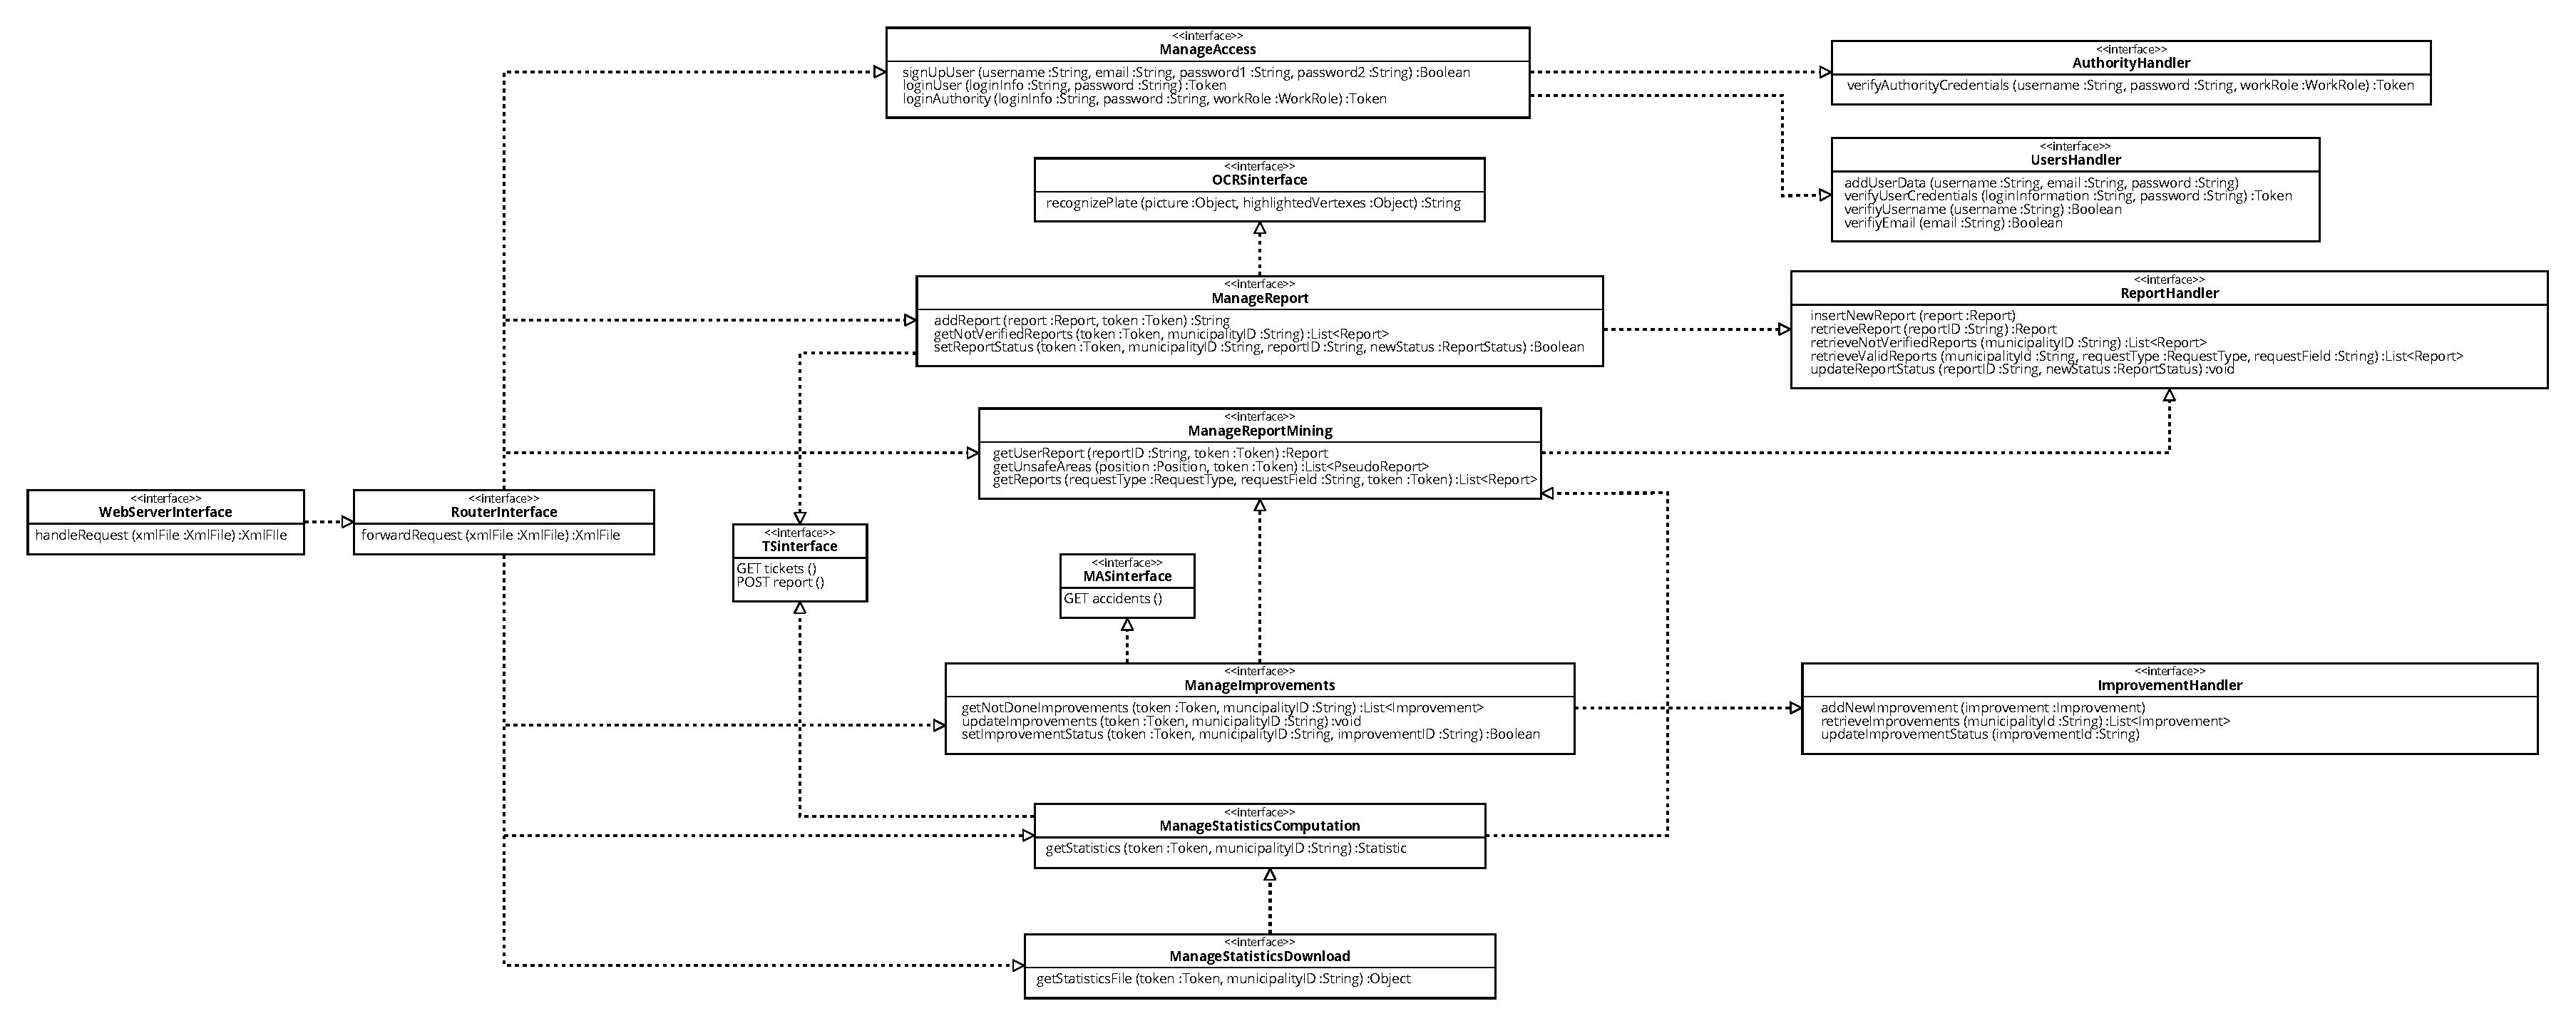
\includegraphics[width=\textwidth]{images/DD2/interfaces.pdf}
					\caption{Component interfaces}
				\end{figure}
			\paragraph{}
				As the development continued, the class diagram introduced in the RASD document has been updated. So we decided to  report here the new version, with classes used by the interfaces described below.
				\begin{figure}[!h]
					\centering
					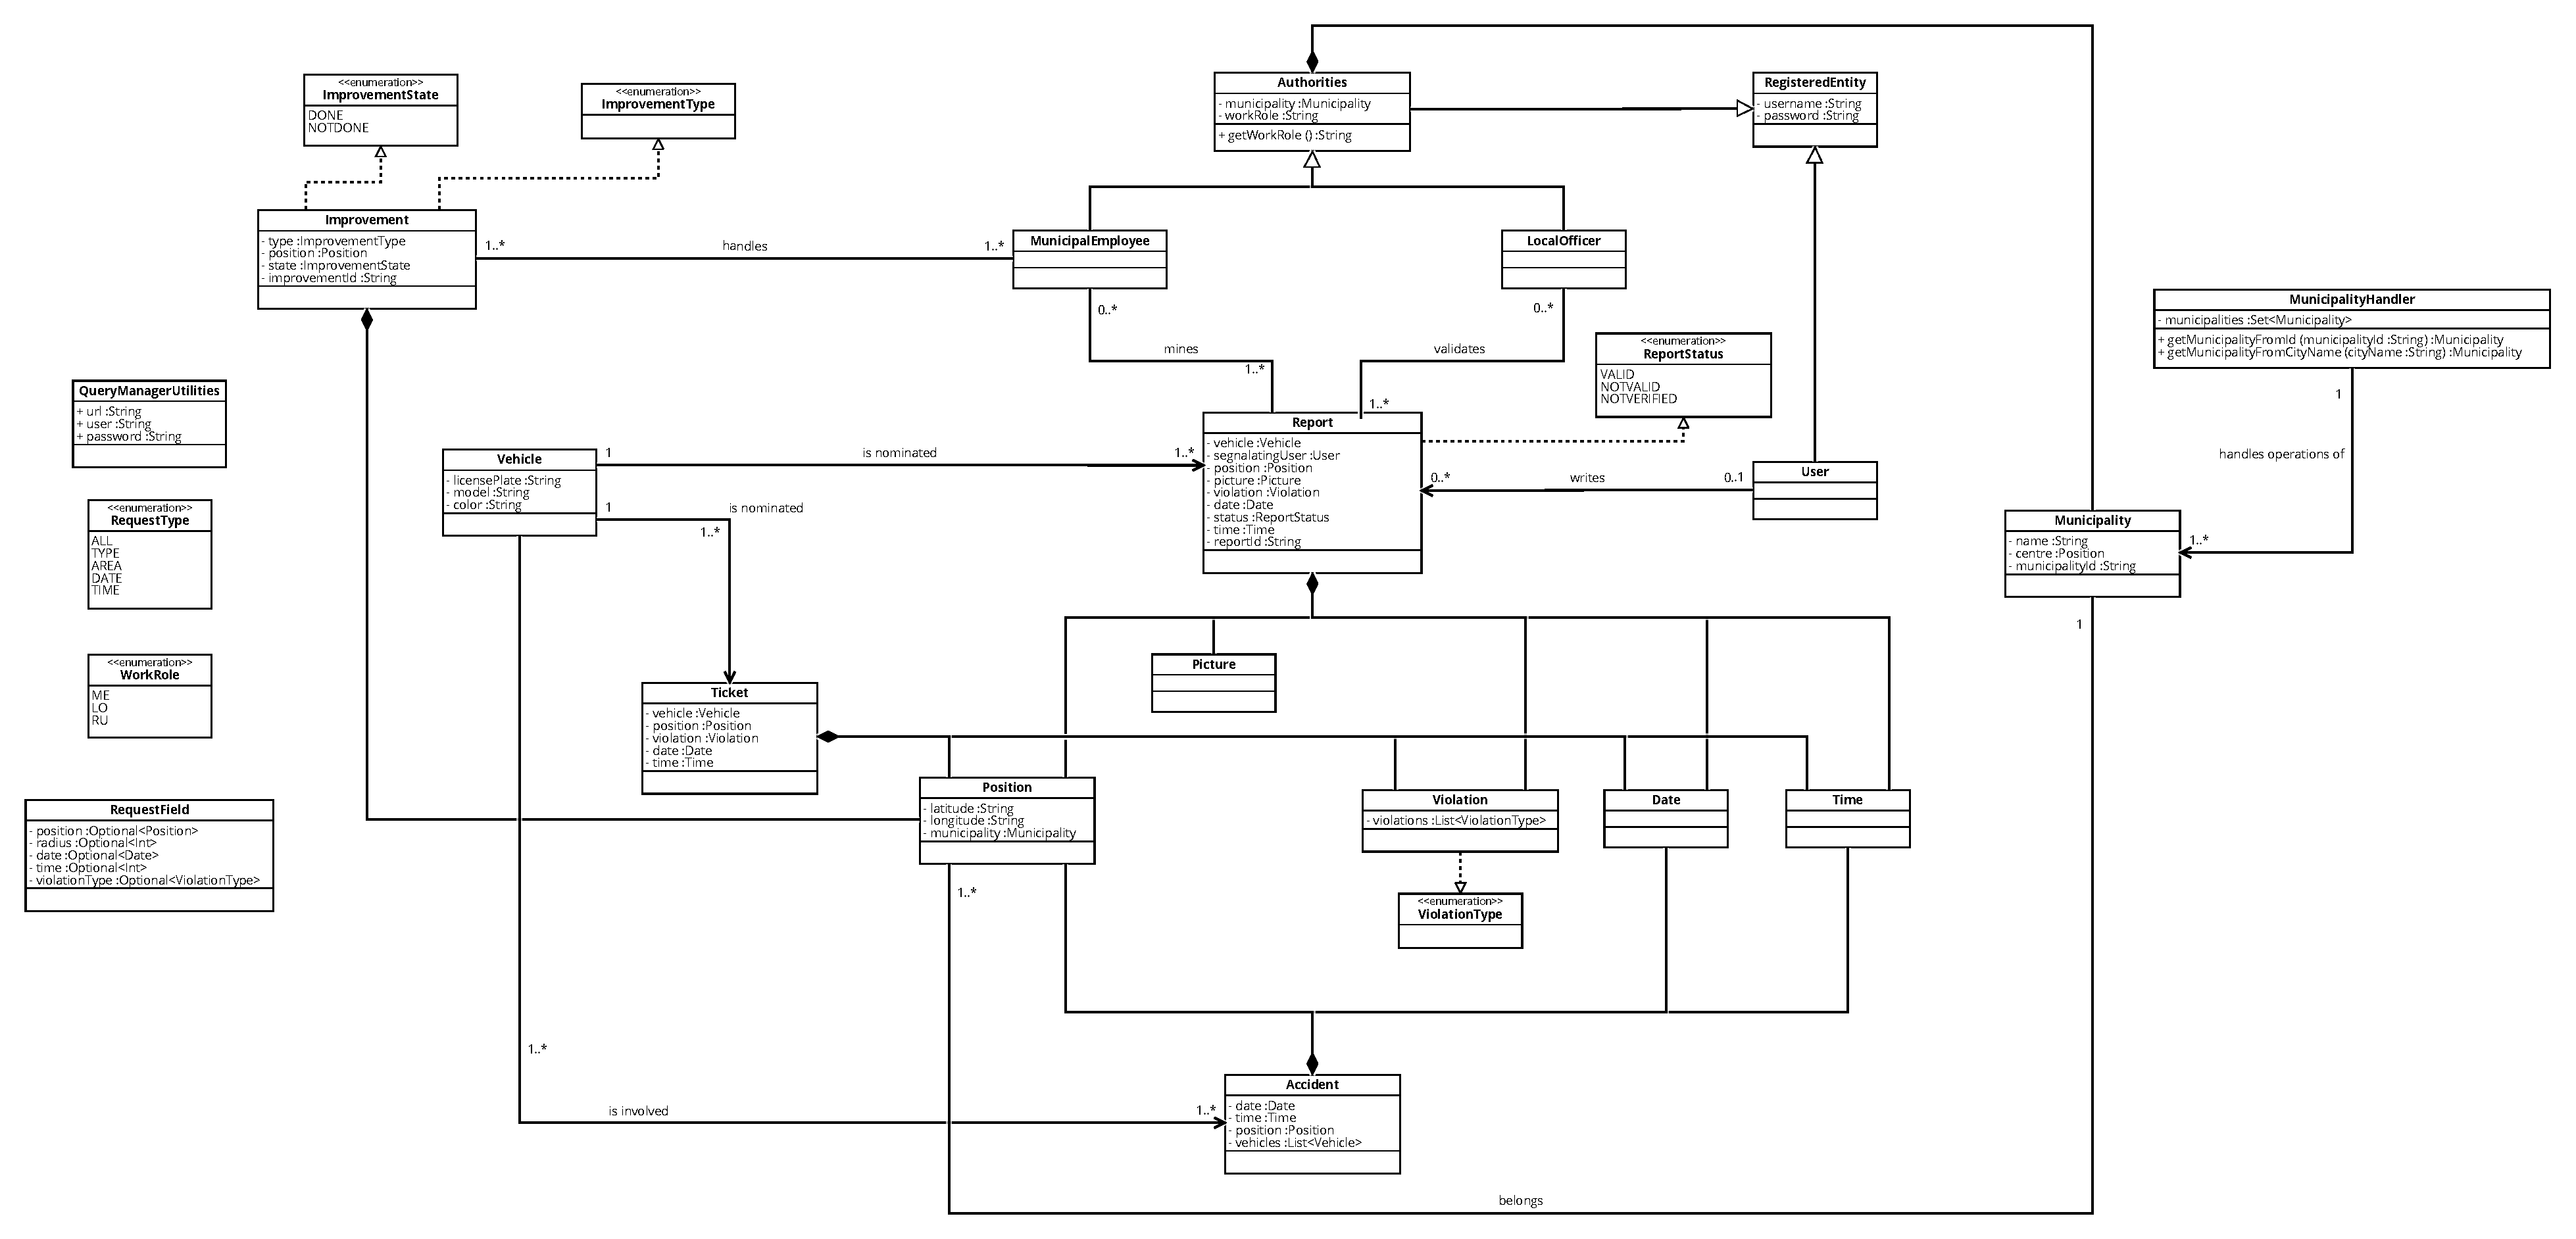
\includegraphics[width=\textwidth]{images/DD2/classDiagram.pdf}
					\caption{Class diagram}
				\end{figure}
			\newpage
			\subsection{Web Server interface and Report interface}
				\paragraph{}
					For the Web server interface and the Report interface a RESTful API has been chosen. Since both interfaces are a vital part of the system and the components that they connect belongs to the part that will be implemented, they will be discussed in depth.
				\subsubsection{REST table of resources}
					\paragraph{}
						The following table represents the logic structures of the resources of the system and the operation that can be done on them (none of them admits DELETE).
						\begin{table}[!h]
							\centering
							\begin{tabular}{L{0.5\textwidth}ccc}
								\toprule
								\textbf{URI}	& \textbf{POST} & \textbf{GET} & \textbf{PUT} \\
								\midrule
								{\ttfamily /users/registration/?id=xxx} & X & - & - \\
								{\ttfamily /users/login/?id=xxx} & - & X & - \\
								{\ttfamily /users/authorities/login/?id=xxx} & - & X & - \\
								{\ttfamily /reports/default} & X & - & - \\
								{\ttfamily /reports/default/?id=xxx} & - & X & - \\
								{\ttfamily /reports/default/unsafearea} & - & X & - \\
								{\ttfamily /reports/notverified/?id=xxx} & - & X & X \\
								{\ttfamily /reports/valid/?id=xxx} & - & X & - \\
								{\ttfamily /improvements/?id=xxx} & - & X & X \\
								{\ttfamily /statistics/visualize/?id=xxx} & - & X & - \\
								{\ttfamily /statistics/download/?id=xxx} & - & X & - \\
							\end{tabular}
							\caption{REST table of resources}
						\end{table}
					\paragraph{}
						"X" : the operation is applicable on the resource
						
						"-" : the operation is inapplicable on the resource
					\clearpage
					\paragraph{}
						Here a quick description of the resources group:
						\begin{itemize}
							\item {\ttfamily /users/*} represents the information related to the users, in particular their account information
							\item {\ttfamily /reports/default/*} represents the resources accessible by the RU, in particular reports and "pseudo report" for the unsafe areas. These resources will be greatly used by the mobile app.
							\item {\ttfamily /reports/notverified/*} contains all the received reports that haven't been immediately discarded by the OCRS but are still on impending evaluation by a LO
							\item {\ttfamily /reports/valid/*} contains all the received reports that have been judged as valid by a LO
							\item {\ttfamily /improvements/*} contains the improvements suggested to a municipality that can be retrieved by a ME
							\item {\ttfamily /statistics/*} contains the statistics that can be retrieved by an authority
						\end{itemize}
				\subsubsection{General request description}
					\paragraph{}
						The data that will be transmitted will be composed of XML files.
						
						To recognize the user who sent a request to the server, the system will employ tokens. A token is a string that is provided to the user as an answer to the login, it contains information on the user and will always be part of the requests, except the login and sign up.
						The contained information will be:
						\begin{itemize}
							\item User type information: the different type users (RU, LO and ME) will be identified in different ways to avoid ambiguity. Moreover the identifier for LO and ME will contain an identifier for the Municipality they work for
							\item User identifier: The single user will be identified to have information on who is making the request and give the correct permission to access data.
							\item Creation time: The token is a "one time only" use. Its validity is fixed and will generally last at least for a session, this permits to recycle pieces of tokens and avoids the malicious use of old ones to get data.
						\end{itemize}
				\clearpage
				\subsubsection{Detailed requests}
					\begin{figure}[!h]
						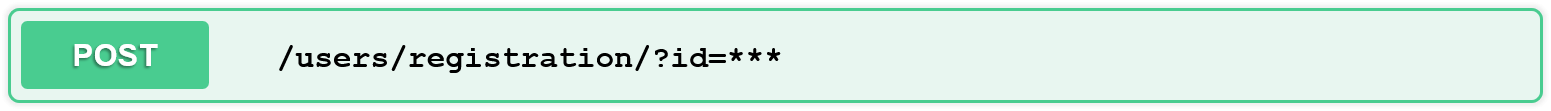
\includegraphics[width=\textwidth]{images/Restful/UserRegistration}
					\end{figure}
						\paragraph{}
						\vspace{-7.5mm}
						This request is used to register a user
					\paragraph{}
						\textcolor{myBlue}{\textit{\textbf{Parameters}}}
						\vspace{-2mm}
						\begin{table}[!h]
							\begin{tabular}{L{0.2\textwidth}L{0.2\textwidth}L{0.48\textwidth}}
								\toprule
								\textbf{Field} & \textbf{Type} & \textbf{Description} \\
								\midrule
								 id & String & The username of the user who is trying to register \\
								 \bottomrule
							\end{tabular}
						\end{table}
					\vspace{-5mm}
					\paragraph{}
						\textcolor{myBlue}{\textit{\textbf{Fields}}}
						\vspace{-2mm}
						\begin{table}[!h]
							\centering
							\begin{tabular}{L{0.25\textwidth}L{0.15\textwidth}L{0.48\textwidth}}
								\toprule
								\textbf{Field} & \textbf{Type} & \textbf{Description} \\
								\midrule
								 email & String & The email of the user \\
								 passwordFirst & String & The password of the user \\
								 passwordSecond & String & The same password as before, used to confirm the first password \\
								 \bottomrule
							\end{tabular}
						\end{table}
					\paragraph{}
						\textcolor{myGreen}{\textit{\textbf{Success 201}}} (resource created)
					\paragraph{}
						\textcolor{myRed}{\textit{\textbf{Error 401}}}
						\vspace{-2mm}
						\begin{table}[!h]
							\begin{tabular}{L{0.3\textwidth}L{0.62\textwidth}}
								\toprule
								\textbf{Field} & \textbf{Description} \\
								\midrule
								 ExistingUsername & Someone with the same username is already registered \\
								 DifferentPassword & The second password is different from the first one \\
								 ExistingMail & This email is already associated with another account \\
								 \bottomrule
							\end{tabular}
						\end{table}
						\clearpage
						\begin{figure}[!h]
							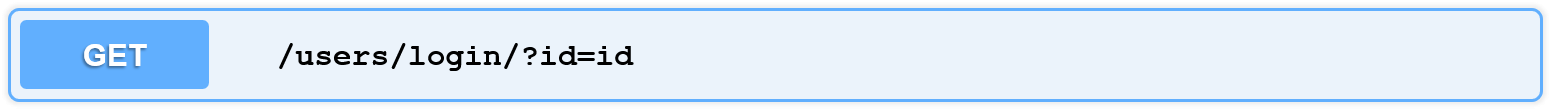
\includegraphics[width=\textwidth]{images/Restful/RULogin}
						\end{figure}
						\paragraph{}
						\vspace{-7.5mm}
						This request allows a RU to login
						\paragraph{}
							\textcolor{myBlue}{\textit{\textbf{Parameters}}}
							\vspace{-2mm}
							\begin{table}[!h]
								\begin{tabular}{L{0.15\textwidth}L{0.15\textwidth}L{0.58\textwidth}}
									\toprule
									\textbf{Field} & \textbf{Type} & \textbf{Description} \\
									\midrule
								 	id & String & The username of the user who is trying to login \\
								 	\bottomrule
								\end{tabular}
							\end{table}
						\paragraph{}
							\textcolor{myBlue}{\textit{\textbf{Fields}}}
							\vspace{-2mm}
							\begin{table}[!h]
								\begin{tabular}{L{0.25\textwidth}L{0.15\textwidth}L{0.48\textwidth}}
									\toprule
									\textbf{Field} & \textbf{Type} & \textbf{Description} \\
									\midrule
								 	loginInformation & String & The email or username of the user \\
								 	password & String & The password of the user \\
								 	\bottomrule
								\end{tabular}
							\end{table}
						\paragraph{}
							\textcolor{myGreen}{\textit{\textbf{Success 200}}} (request ok)
							\vspace{-2mm}
							\begin{table}[!h]
								\begin{tabular}{L{0.2\textwidth}L{0.15\textwidth}L{0.53\textwidth}}
									\toprule
									\textbf{Field} & \textbf{Type} & \textbf{Description} \\
									\midrule
									token & String & A token that represents the user \\
									reportIDs & String[] & The list of id associated with the reports uploaded by the user \\
								 	\bottomrule
								\end{tabular}
							\end{table}
						\vspace{-5mm}
						\paragraph{}
							\textcolor{myRed}{\textit{\textbf{Error 401}}} (Unauthorized)
							\vspace{-2mm}
							\begin{table}[!h]
								\begin{tabular}{L{0.4\textwidth}L{0.52\textwidth}}
									\toprule
									\textbf{Field} & \textbf{Description} \\
									\midrule
								  	WrongUsernameOrPassword & The written username and password does not correspond to any existing user \\
								 	\bottomrule
								\end{tabular}
							\end{table}
							
						\clearpage
						\begin{figure}[!h]
							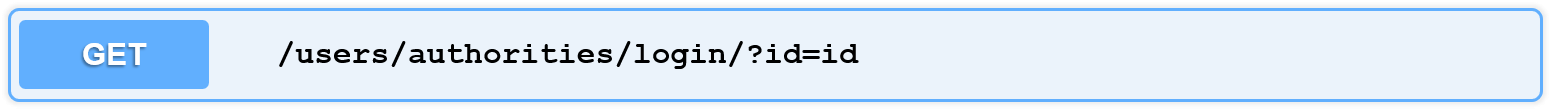
\includegraphics[width=\textwidth]{images/Restful/AuthorityLogin}
						\end{figure}
						\paragraph{}
						\vspace{-7.5mm}
						This request allows a ME or LO to login
						\paragraph{}
							\textcolor{myBlue}{\textit{\textbf{Parameters}}}
							\vspace{-2mm}
							\begin{table}[!h]
								\begin{tabular}{L{0.2\textwidth}L{0.2\textwidth}L{0.48\textwidth}}
									\toprule
									\textbf{Field} & \textbf{Type} & \textbf{Description} \\
									\midrule
								 	id & String & The username of the user who is trying to login \\
								 	\bottomrule
								\end{tabular}
							\end{table}
						\paragraph{}
							\vspace{-5mm}
							\textcolor{myBlue}{\textit{\textbf{Fields}}}
							\vspace{-2mm}
							\begin{table}[!h]
								\begin{tabular}{L{0.25\textwidth}L{0.15\textwidth}L{0.48\textwidth}}
									\toprule
									\textbf{Field} & \textbf{Type} & \textbf{Description} \\
									\midrule
								 	loginInformation & String  & The username of the user \\
								 	password & String & The password of the user \\
								 	workRole & String & This will be 'ME' or 'LO' \\
								 	\bottomrule
								\end{tabular}
							\end{table}
						\paragraph{}
							\textcolor{myGreen}{\textit{\textbf{Success 200}}} (request ok)
							\vspace{-2mm}
							\begin{table}[!h]
								\begin{tabular}{L{0.25\textwidth}L{0.1\textwidth}L{0.53\textwidth}}
									\toprule
									\textbf{Field} & \textbf{Type} & \textbf{Description} \\
									\midrule
									token & String & A token that represents the user and the municipality he/she works in \\
									municipalityID & String & The id of the municipality where the ME or LO works, this will be a parameter for the following requests \\
								 	\bottomrule
								\end{tabular}
							\end{table}
						\vspace{-5mm}
						\paragraph{}
							\textcolor{myRed}{\textit{\textbf{Error 401}}} (Unauthorized)
							\vspace{-2mm}
							\begin{table}[!h]
								\begin{tabular}{L{0.4\textwidth}L{0.52\textwidth}}
									\toprule
									\textbf{Field} & \textbf{Description} \\
									\midrule
								  	WrongUsernameOrPassword & The written username and password does not correspond to any existing user \\
								  	NotCorrespondingRole & The selected work role does not correspond to the user which given login and password corresponds to \\
								 	\bottomrule
								\end{tabular}
							\end{table}
							
						\clearpage
						\begin{figure}[!h]
						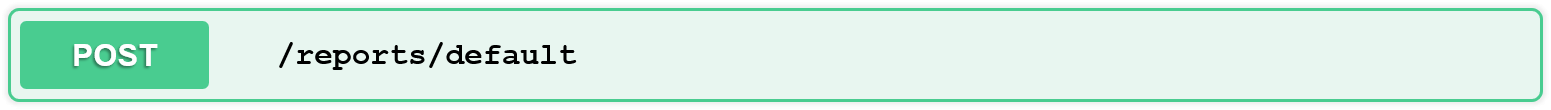
\includegraphics[width=\textwidth]{images/Restful/AddReport}
						\end{figure}
						\paragraph{}
						\vspace{-7.5mm}
						This request adds a report to the system
						\paragraph{}
							\textcolor{myBlue}{\textit{\textbf{Fields}}}
							\vspace{-2mm}
							\begin{table}[!h]
								\begin{tabular}{L{0.3\textwidth}L{0.15\textwidth}L{0.43\textwidth}}
									\toprule
									\textbf{Field} & \textbf{Type} & \textbf{Description} \\
									\midrule
								 	vehicle & Object & The vehicle information \\
								 	\hspace{2.5mm}$\hookrightarrow$ licensePlate & String & The license plate of the vehicle \\
								 	position & Object & The position, expressed in DMS, of the vehicle when the report was submitted  \\
								 	\hspace{2.5mm}$\hookrightarrow$ latitude & String & The latitude where the vehicle was recorded to be \\
								 	\hspace{2.5mm}$\hookrightarrow$ longitude & String & The longitude where the vehicle was recorded to be \\
								 	picture & Object & Representation of the image of the vehicle \\
								 	violation & Object[] & An array of the type of violation \\
								 	\hspace{2.5mm}$\hookrightarrow$ violationType & String & The type of violation \\
								 	date & String & The datetime in \newline dd-MM-yyyyThh:mm:ss format \\
								 	highlightVertexes & Object & The coordinates on the picture of where the license plate is located \\
								 	\hspace{2.5mm}$\hookrightarrow$ vertexOne & Number[] & The coordinates (on the picure) of the top-left vertex \\
								 	\hspace{2.5mm}$\hookrightarrow$ vertexTwo & Number[] & The coordinates (on the picture) of the bottom-right vertex \\
								 	\bottomrule
								\end{tabular}
							\end{table}
						\paragraph{}
							\textcolor{myGreen}{\textit{\textbf{Success 201}}} (resource created)
							\vspace{-2mm}
							\begin{table}[!h]
								\begin{tabular}{L{0.15\textwidth}L{0.15\textwidth}L{0.58\textwidth}}
									\toprule
									\textbf{Field} & \textbf{Type} & \textbf{Description} \\
									\midrule
									id & String & The id that the system has assigned to the sent report. This id will uniquely identify the report and will also contain information about the user which sent it\\
								 	\bottomrule
								\end{tabular}
							\end{table}
						
						\clearpage
						\begin{figure}[!h]
							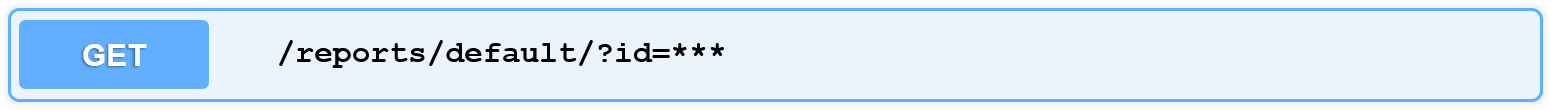
\includegraphics[width=\textwidth]{images/Restful/RetrieveReport}
						\end{figure}
						\paragraph{}
						\vspace{-7.5mm}
						This request retrieves a report form the system.
						\paragraph{}
							\textcolor{myBlue}{\textbf{\textit{Parameters}}}
							\vspace{-2mm}
							\begin{table}[!h]
								\begin{tabular}{L{0.15\textwidth}L{0.15\textwidth}L{0.58\textwidth}}
									\toprule
									\textbf{Field} & \textbf{Type} & \textbf{Description} \\
									\midrule
								 	id & String & The id that uniquely identifies the report that the user wants to see \\
								 	\bottomrule
								\end{tabular}
							\end{table}
						\paragraph{}
							\textcolor{myGreen}{\textit{\textbf{Success 200}}} (request ok)
							\vspace{-2mm}
							\begin{table}[!h]
								\begin{tabular}{L{0.3\textwidth}L{0.15\textwidth}L{0.43\textwidth}}
									\toprule
									\textbf{Field} & \textbf{Type} & \textbf{Description} \\
									\midrule
								 	vehicle & Object & The vehicle information \\
								 	\hspace{2.5mm}$\hookrightarrow$licensePlate & String & The license plate of the vehicle \\
								 	position & Object & The position, expressed in DMS, of the vehicle when the report was submitted  \\
								 	\hspace{2.5mm}$\hookrightarrow$latitude & String & The latitude where the vehicle was recorded to be \\
								 	\hspace{2.5mm}$\hookrightarrow$longitude & String & The longitude where the vehicle was recorded to be \\
								 	picture & Object & Representation of the image of the vehicle \\
								 	violation & Object[] & An array of the type of violation \\
								 	\hspace{2.5mm}$\hookrightarrow$violationType & String & The type of violation \\
								 	date & String & The datetime in \newline dd-MM-yyyyThh:mm:ss format \\
								 	highlightVertexes & Object & The coordinates on the picture of where the license plate is located \\
								 	\hspace{2.5mm}$\hookrightarrow$vertexOne & Number[] & The coordinates (on the picure) of the top-left vertex \\
								 	\hspace{2.5mm}$\hookrightarrow$vertexTwo & Number[] & The coordinates (on the picture) of the bottom-right vertex \\
								 	\bottomrule
								\end{tabular}
							\end{table}
						\paragraph{}
							\textcolor{myRed}{\textit{\textbf{Error 403}}} (Forbidden)
							\vspace{-2mm}
							\begin{table}[!h]
								\begin{tabular}{L{0.35\textwidth}L{0.57\textwidth}}
									\toprule
									\textbf{Field} & \textbf{Description} \\
									\midrule
								  	 NoReportError & The requested resource caused an error on the database, this could both mean that the resource was not found on the database or that the database had internal error or an error on the connection \\
								 	\bottomrule
								\end{tabular}
							\end{table}
	
							\clearpage
							\begin{figure}[!h]
								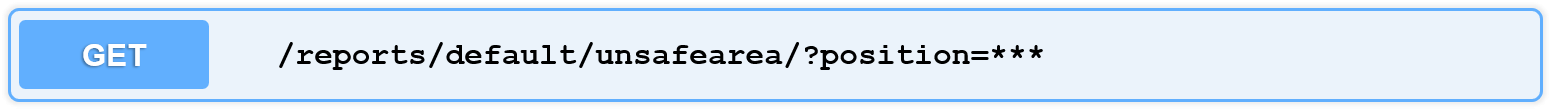
\includegraphics[width=\textwidth]{images/Restful/GetUnsafeAreas}
							\end{figure}
						\paragraph{}
						\vspace{-7.5mm}
						This request retrieves the type of violations in certain area.
						\paragraph{}
							\textcolor{myBlue}{\textit{\textbf{Fields}}}
							\vspace{-2mm}
							\begin{table}[!h]
								\begin{tabular}{L{0.2\textwidth}L{0.13\textwidth}L{0.56\textwidth}}
									\toprule
									\textbf{Field} & \textbf{Type} & \textbf{Description} \\
									\midrule
								 	position & Object & The position, expressed in DMS, of the center of the area which the RU wants to know about \\
								 	\hspace{2.5mm}$\hookrightarrow$latitude & String & The latitude where the vehicle was recorded to be \\
								 	\hspace{2.5mm}$\hookrightarrow$longitude & String & The longitude where the vehicle was recorded to be \\
								 	\bottomrule
								\end{tabular}
							\end{table}
						\paragraph{}
							\textcolor{myGreen}{\textit{\textbf{Success 200}}} (request ok)
							\vspace{-2mm}
							\begin{table}[!h]
								\begin{tabular}{L{0.3\textwidth}L{0.15\textwidth}L{0.43\textwidth}}
									\toprule
									\textbf{Field} & \textbf{Type} & \textbf{Description} \\
									\midrule
									pseudoReport & Object[] & The list of partial reports that can be seen bya a RU \\
									\hspace{2.5mm}$\hookrightarrow$position & Object & The position, expressed in DMS, of the vehicle when the report was submitted  \\
									\hspace{6.5mm}$\hookrightarrow$latitude & String & The latitude where the vehicle was recorded to be \\
									\hspace{6.5mm}$\hookrightarrow$longitude & String & The longitude where the vehicle was recorded to be \\
									\hspace{2.5mm}$\hookrightarrow$violation & Object[] & An array of the type of violation \\
									\hspace{6.5mm}$\hookrightarrow$violationType & String & The type of violation \\
								 	\bottomrule
								\end{tabular}
							\end{table}
						\paragraph{}
							\textcolor{myRed}{\textit{\textbf{Error 404}}} (Resource not found)
							\vspace{-2mm}
							\begin{table}[!h]
								\begin{tabular}{L{0.3\textwidth}L{0.62\textwidth}}
									\toprule
									\textbf{Field} & \textbf{Description} \\
									\midrule
								  	 NoReportError & The requested resource caused an error on the database, this could both mean that the resource was not found on the database or that the database had internal error or an error on the connection \\
								 	\bottomrule
								\end{tabular}
							\end{table}
						
						\clearpage
						\begin{figure}[!h]
							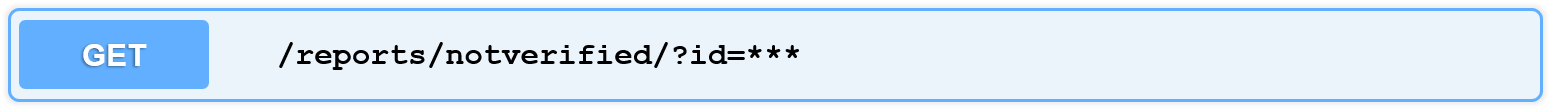
\includegraphics[width=\textwidth]{images/Restful/ToValidate}
						\end{figure}
						\paragraph{}
						\vspace{-7.5mm}
						This request retrieves the reports that are waiting for validation in a certain municipality.
						\paragraph{}
							\textcolor{myBlue}{\textit{\textbf{Parameters}}}
							\vspace{-2mm}
							\begin{table}[!h]
								\begin{tabular}{L{0.15\textwidth}L{0.15\textwidth}L{0.58\textwidth}}
									\toprule
									\textbf{Field} & \textbf{Type} & \textbf{Description} \\
									\midrule
								 	id & String & The id that uniquely identifies the municipality which the LO works for \\
								 	\bottomrule
								\end{tabular}
							\end{table}
						\paragraph{}
							\textcolor{myGreen}{\textit{\textbf{Success 200}}} (request ok)
							\vspace{-2mm}
							\begin{table}[!h]
								\begin{tabular}{L{0.3\textwidth}L{0.15\textwidth}L{0.43\textwidth}}
									\toprule
									\textbf{Field} & \textbf{Type} & \textbf{Description} \\
									\midrule
									reports & Object[] & A list of the valid reports of a certain municipality \\
									\hspace{2.5mm}$\hookrightarrow$reportId & String & The string that uniquely identifies a report \\
									\hspace{2.5mm}$\hookrightarrow$vehicle & Object & The vehicle information \\
									\hspace{6.5mm}$\hookrightarrow$licensePlate & String & The license plate of the vehicle \\
									\hspace{2.5mm}$\hookrightarrow$position & Object & The position, expressed in DMS, of the vehicle when the report was submitted  \\
									\hspace{6.5mm}$\hookrightarrow$latitude & String & The latitude where the vehicle was recorded to be \\
									\hspace{6.5mm}$\hookrightarrow$longitude & String & The longitude where the vehicle was recorded to be \\
									\hspace{2.5mm}$\hookrightarrow$picture & Object & Representation of the image of the vehicle \\
									\hspace{2.5mm}$\hookrightarrow$violation & Object[] & An array of the type of violation \\
									\hspace{6.5mm}$\hookrightarrow$violationType & String & The type of violation \\
									\hspace{2.5mm}$\hookrightarrow$date & String & The datetime in \newline dd-MM-yyyyThh:mm:ss format \\
								 	\bottomrule
								\end{tabular}
							\end{table}
						\paragraph{}
							\textcolor{myRed}{\textit{\textbf{Error 403}}} (Forbidden)
							\vspace{-2mm}
							\begin{table}[!h]
								\begin{tabular}{L{0.3\textwidth}L{0.62\textwidth}}
									\toprule
									\textbf{Field} & \textbf{Description} \\
									\midrule
								  	UserNotAuthorized & The id of the municipality and the token of the user have been analyzed. It was found that the user was not an LO or the LO's municipality was not the one of the reports requested \\
								 	\bottomrule
								\end{tabular}
							\end{table}
							
							\clearpage
							\begin{figure}[!h]
								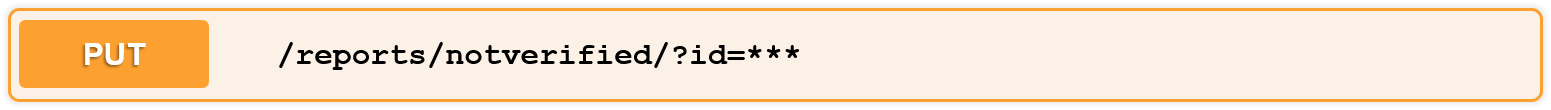
\includegraphics[width=\textwidth]{images/Restful/ValidateReport}
							\end{figure}
						\paragraph{}
						\vspace{-7.5mm}
						This request modifies the status of a report
						\paragraph{}
							\textcolor{myBlue}{\textit{\textbf{Parameters}}}
							\vspace{-2mm}
							\begin{table}[!h]
								\begin{tabular}{L{0.15\textwidth}L{0.15\textwidth}L{0.58\textwidth}}
									\toprule
									\textbf{Field} & \textbf{Type} & \textbf{Description} \\
									\midrule
								 	id & String & The id that uniquely identifies the municipality which the LO works for \\
								 	\bottomrule
								\end{tabular}
							\end{table}
						\vspace{-5mm}
						\paragraph{}
							\textcolor{myBlue}{\textit{\textbf{Fields}}}
							\vspace{-2mm}
							\begin{table}[!h]
								\begin{tabular}{L{0.2\textwidth}L{0.15\textwidth}L{0.53\textwidth}}
									\toprule
									\textbf{Field} & \textbf{Type} & \textbf{Description} \\
									\midrule
								 	id & String & The id of the report \\
								 	newStatus & String & The result of the validation performed by the LO \\
								 	\bottomrule
								\end{tabular}
							\end{table}
						\paragraph{}
							\textcolor{myRed}{\textit{\textbf{Error 403}}} (Forbidden)
							\vspace{-2mm}
							\begin{table}[!h]
								\begin{tabular}{L{0.3\textwidth}L{0.62\textwidth}}
									\toprule
									\textbf{Field} & \textbf{Description} \\
									\midrule
								  	UserNotAuthorized & The id of the municipality and the token of the user have been analyzed. It was found that the user was not an LO or the LO's municipality was not the one of the reports requested \\
								 	\bottomrule
								\end{tabular}
							\end{table}
							
						\clearpage
						\begin{figure}[!h]
							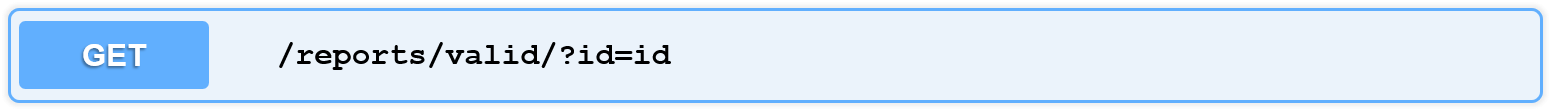
\includegraphics[width=\textwidth]{images/Restful/ValidReports}
						\end{figure}
						\paragraph{}
						\vspace{-7.5mm}
						This request gets all the valid reports in a certain municipality.
						\paragraph{}
							\textcolor{myBlue}{\textit{\textbf{Parameters}}}
							\vspace{-2mm}
							\begin{table}[!h]
								\begin{tabular}{L{0.1\textwidth}L{0.15\textwidth}L{0.63\textwidth}}
									\toprule
									\textbf{Field} & \textbf{Type} & \textbf{Description} \\
									\midrule
								 	id & String & The id that uniquely identifies the municipality which the LO works for \\
								 	\bottomrule
								\end{tabular}
							\end{table}
						\vspace{-5mm}
						\paragraph{}
							\textcolor{myBlue}{\textit{\textbf{Fields}}}
							\vspace{-2mm}
							\begin{table}[!h]
								\begin{tabular}{L{0.2\textwidth}L{0.15\textwidth}L{0.53\textwidth}}
									\toprule
									\textbf{Field} & \textbf{Type} & \textbf{Description} \\
									\midrule
								 	requestType & String & The type of request issued (i.e. "by area") \\
								 	requestField & String & The field that contains precise information on the request \\
								 	\bottomrule
								\end{tabular}
							\end{table}
						\paragraph{}
							\textcolor{myGreen}{\textit{\textbf{Success 200}}} (request ok)
							\vspace{-2mm}
							\begin{table}[!h]
								\begin{tabular}{L{0.3\textwidth}L{0.15\textwidth}L{0.43\textwidth}}
									\toprule
									\textbf{Field} & \textbf{Type} & \textbf{Description} \\
									\midrule
									reports & Object[] & A list of the valid reports of a certain municipality \\
									\hspace{2.5mm}$\hookrightarrow$reportId & String & The string that uniquely identifies a report \\
									\hspace{2.5mm}$\hookrightarrow$vehicle & Object & The vehicle information \\
									\hspace{5mm}licensePlate & String & The license plate of the vehicle \\
									\hspace{2.5mm}$\hookrightarrow$position & Object & The position, expressed in DMS, of the vehicle when the report was submitted  \\
									\hspace{6.5mm}$\hookrightarrow$latitude & String & The latitude where the vehicle was recorded to be \\
									\hspace{6.5mm}$\hookrightarrow$longitude & String & The longitude where the vehicle was recorded to be \\
									\hspace{2.5mm}$\hookrightarrow$picture & Object & Representation of the image of the vehicle \\
									\hspace{2.5mm}$\hookrightarrow$violation & Object[] & An array of the type of violation \\
									\hspace{6.5mm}$\hookrightarrow$violationType & String & The type of violation \\
									\hspace{2.5mm}$\hookrightarrow$date & String & The datetime in \newline dd-MM-yyyyThh:mm:ss format \\
								 	\bottomrule
								\end{tabular}
							\end{table}
						\clearpage
						\paragraph{}
						\vspace{-5mm}
							\textcolor{myRed}{\textit{\textbf{Error 403}}} (Forbidden)
							\vspace{-2mm}
							\begin{table}[!h]
								\begin{tabular}{L{0.3\textwidth}L{0.62\textwidth}}
									\toprule
									\textbf{Field} & \textbf{Description} \\
									\midrule
								  	UserNotAuthorized & The id of the municipality and the token of the user have been analyzed. It was found that the user was not an LO or the LO's  municipality was not the one of the reports requested  \\
								 	\bottomrule
								\end{tabular}
							\end{table}
						\vspace{-5mm}
						\paragraph{}
							\textcolor{myRed}{\textit{\textbf{Error 404}}} (Resource not found)
							\vspace{-2mm}
							\begin{table}[!h]
								\begin{tabular}{L{0.25\textwidth}L{0.67\textwidth}}
									\toprule
									\textbf{Field} & \textbf{Description} \\
									\midrule
								  	 NoReportError & The requested resource caused an error on the database, this could both mean that the resource was not found on the database or that the database had internal error or an error on the connection \\ 
								 	\bottomrule
								\end{tabular}
							\end{table}
						
						\clearpage
						\begin{figure}[!h]
							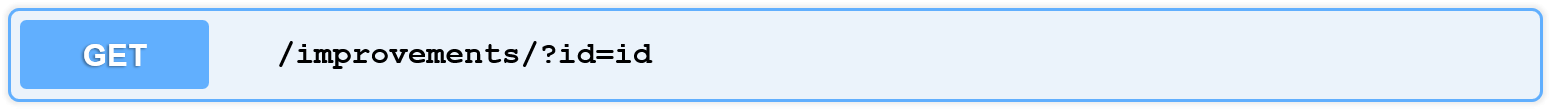
\includegraphics[width=\textwidth]{images/Restful/GetImprovements}
						\end{figure}
						\paragraph{}
						\vspace{-7.5mm}
						This request retrieves all the suggested improvements in a certain municipality
						\paragraph{}
							\textcolor{myBlue}{\textit{\textbf{Parameters}}}
							\vspace{-2mm}
							\begin{table}[!h]
								\begin{tabular}{L{0.15\textwidth}L{0.15\textwidth}L{0.58\textwidth}}
									\toprule
									\textbf{Field} & \textbf{Type} & \textbf{Description} \\
									\midrule
								 	id & String & The id that uniquely identifies the municipality which the ME works for \\
								 	\bottomrule
								\end{tabular}
							\end{table}
						\paragraph{}
							\textcolor{myGreen}{\textit{\textbf{Success 200}}} (request ok)
							\vspace{-2mm}
							\begin{table}[!h]
								\begin{tabular}{L{0.3\textwidth}L{0.15\textwidth}L{0.43\textwidth}}
									\toprule
									\textbf{Field} & \textbf{Type} & \textbf{Description} \\
									\midrule
									improvements & Object[] & The list of suggested improvements \\
									\hspace{2.5mm}$\hookrightarrow$type & String & The type of the improvement\\
									\hspace{2.5mm}$\hookrightarrow$position & Object & The position of the improvement expresses in DMS \\
									\hspace{6.5mm}$\hookrightarrow$latitude & String & The latitude where the suggested improvement will be expected to be \\
									\hspace{6.5mm}$\hookrightarrow$longitude & String & The longitude where the suggested improvement will be expected to be  \\
									\hspace{2.5mm}$\hookrightarrow$state & String & The status of the improvement, "DONE" or "NOT DONE" \\
									\hspace{2.5mm}$\hookrightarrow$improvementId & String & The id that uniquely identifies the improvement on the database \\
								 	\bottomrule
								\end{tabular}
							\end{table}
						\vspace{-5mm}
						\paragraph{}
							\textcolor{myRed}{\textit{\textbf{Error 403}}} (Forbidden)
							\vspace{-2mm}
							\begin{table}[!h]
								\begin{tabular}{L{0.3\textwidth}L{0.62\textwidth}}
									\toprule
									\textbf{Field} & \textbf{Description} \\
									\midrule
								  	UserNotAuthorized & The id of the municipality and the token of the user have been analyzed. It was found that the user was not an ME or the ME's  municipality was not the one of the reports requested  \\
								 	\bottomrule
								\end{tabular}
							\end{table}
						\vspace{-5mm}
						\paragraph{}
							\textcolor{myRed}{\textit{\textbf{Error 404}}} (Resource not found)
							\vspace{-2mm}
							\begin{table}[!h]
								\begin{tabular}{L{0.3\textwidth}L{0.62\textwidth}}
									\toprule
									\textbf{Field} & \textbf{Description} \\
									\midrule
								  	NotEnoughReportError & The requested improvements could not be found on the database and the available information on the Municipality is not enough to compute correct suggestions \\
								 	\bottomrule
								\end{tabular}
							\end{table}
						
						\clearpage
						\begin{figure}[!h]
							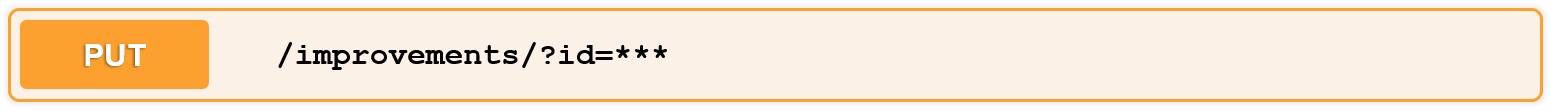
\includegraphics[width=\textwidth]{images/Restful/DoImprovement}
						\end{figure}
						\paragraph{}
						\vspace{-7.5mm}
						This request modifies the status of an improvement from "not done" to "done"
						\paragraph{}
							\textcolor{myBlue}{\textit{\textbf{Parameters}}}
							\vspace{-2mm}
							\begin{table}[!h]
								\begin{tabular}{L{0.15\textwidth}L{0.15\textwidth}L{0.58\textwidth}}
									\toprule
									\textbf{Field} & \textbf{Type} & \textbf{Description} \\
									\midrule
								 	id & String & The id that uniquely identifies the municipality which the LO works for \\
								 	\bottomrule
								\end{tabular}
							\end{table}
						\paragraph{}
						\vspace{-5mm}
							\textcolor{myBlue}{\textit{\textbf{Fields}}}
							\vspace{-2mm}
							\begin{table}[!h]
								\begin{tabular}{L{0.2\textwidth}L{0.15\textwidth}L{0.53\textwidth}}
									\toprule
									\textbf{Field} & \textbf{Type} & \textbf{Description} \\
									\midrule
								 	improvementId & String & The id that uniquely identifies the improvement on the database \\
								 	\bottomrule
								\end{tabular}
							\end{table}
						\paragraph{}
							\textcolor{myRed}{\textit{\textbf{Error 403}}} (Forbidden)
							\vspace{-2mm}
							\begin{table}[!h]
								\begin{tabular}{L{0.3\textwidth}L{0.62\textwidth}}
									\toprule
									\textbf{Field} & \textbf{Description} \\
									\midrule
								  	UserNotAuthorized & The id of the municipality and the token of the user have been analyzed. It was found that the user was not an ME or the ME's municipality was not the one of the reports requested \\
								 	\bottomrule
								\end{tabular}
							\end{table}
							
						\clearpage
						\begin{figure}[!h]
							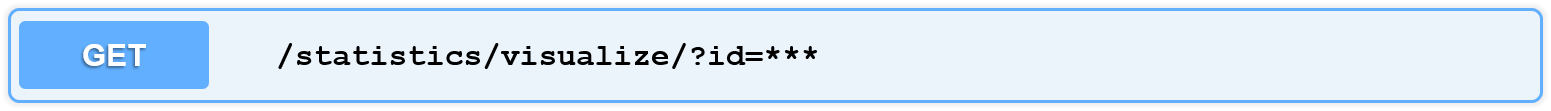
\includegraphics[width=\textwidth]{images/Restful/GetStatistics}
						\end{figure}
						\paragraph{}
						\vspace{-7.5mm}
						This request gets the available statistics on a certain municipality and lets the ME visualize them.
						\paragraph{}
							\textcolor{myBlue}{\textit{\textbf{Parameters}}}
							\vspace{-2mm}
							\begin{table}[!h]
								\begin{tabular}{L{0.15\textwidth}L{0.15\textwidth}L{0.58\textwidth}}
									\toprule
									\textbf{Field} & \textbf{Type} & \textbf{Description} \\
									\midrule
								 	id & String & The id that uniquely identifies the municipality which the LO works for \\
								 	\bottomrule
								\end{tabular}
							\end{table}
						\paragraph{}
							\textcolor{myGreen}{\textit{\textbf{Success 200}}} (request ok)
							\vspace{-2mm}
							\begin{table}[!h]
								\begin{tabular}{L{0.3\textwidth}L{0.15\textwidth}L{0.43\textwidth}}
									\toprule
									\textbf{Field} & \textbf{Type} & \textbf{Description} \\
									\midrule
									statistics & Object[] & The various statistics \\
									\hspace{2.5mm}$\hookrightarrow$firstFieldName & String & The name of the first field of the graph \\
									\hspace{2.5mm}$\hookrightarrow$secondFieldName & String & The name of the second field of the graph \\
									\hspace{2.5mm}$\hookrightarrow$firstFieldValues & Number[] & The values of the first field \\
									\hspace{2.5mm}$\hookrightarrow$secondFieldValues & Number[] & The value of the second field \\
								 	\bottomrule
								\end{tabular}
							\end{table}
						\paragraph{}
							\vspace{-5mm}
							\textcolor{myRed}{\textit{\textbf{Error 403}}} (Forbidden)
							\vspace{-2mm}
							\begin{table}[!h]
								\begin{tabular}{L{0.3\textwidth}L{0.62\textwidth}}
									\toprule
									\textbf{Field} & \textbf{Description} \\
									\midrule
								  	UserNotAuthorized & The id of the municipality and the token of the user have been analyzed. It was found that the user was not an ME or the ME's  municipality was not the one of the reports requested  \\
								 	\bottomrule
								\end{tabular}
							\end{table}
						\vspace{-5mm}
						\paragraph{}
							\textcolor{myRed}{\textit{\textbf{Error 404}}} (Resource not found)
							\vspace{-2mm}
							\begin{table}[!h]
								\begin{tabular}{L{0.3\textwidth}L{0.62\textwidth}}
									\toprule
									\textbf{Field} & \textbf{Description} \\
									\midrule
								  	NotEnoughReportError & The requested statistics could not be found on the database and the available information on the Municipality is not enough to compute accurate statistics \\
								 	\bottomrule
								\end{tabular}
							\end{table}
						
						\clearpage
						\begin{figure}
							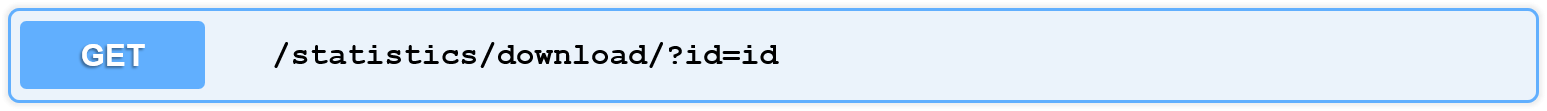
\includegraphics[width=\textwidth]{images/Restful/DownloadStatistics}
						\end{figure}
						\paragraph{}
						\vspace{-7.5mm}
						This request gets the url of the pdf file where the visualized statistics are written
						\paragraph{}
							\textcolor{myBlue}{\textit{\textbf{Parameters}}}
							\vspace{-2mm}
							\begin{table}[!h]
								\begin{tabular}{L{0.15\textwidth}L{0.15\textwidth}L{0.58\textwidth}}
									\toprule
									\textbf{Field} & \textbf{Type} & \textbf{Description} \\
									\midrule
								 	id & String & The id that uniquely identifies the municipality which the LO works for \\
								 	\bottomrule
								\end{tabular}
							\end{table}
						\paragraph{}
							\textcolor{myGreen}{\textit{\textbf{Success 200}}} (request ok)
							\vspace{-2mm}
							\begin{table}[!h]
								\begin{tabular}{L{0.15\textwidth}L{0.15\textwidth}L{0.58\textwidth}}
									\toprule
									\textbf{Field} & \textbf{Type} & \textbf{Description} \\
									\midrule
									url & String & The url where the ME can download the pdf file \\
								 	\bottomrule
								\end{tabular}
							\end{table}
						\paragraph{}
							\vspace{-5mm}
							\textcolor{myRed}{\textit{\textbf{Error 403}}} (Forbidden)
							\vspace{-2mm}
							\begin{table}[!h]
								\begin{tabular}{L{0.3\textwidth}L{0.62\textwidth}}
									\toprule
									\textbf{Field} & \textbf{Description} \\
									\midrule
								  	UserNotAuthorized & The id of the municipality and the token of the user have been analyzed. It was found that the user was not an ME or the ME's  municipality was not the one of the reports requested \\
								 	\bottomrule
								\end{tabular}
							\end{table}
						\vspace{-5mm}
						\paragraph{}
							\textcolor{myRed}{\textit{\textbf{Error 404}}} (Resource not found)
							\vspace{-2mm}
							\begin{table}[!h]
								\begin{tabular}{L{0.35\textwidth}L{0.57\textwidth}}
									\toprule
									\textbf{Field} & \textbf{Description} \\
									\midrule
								  	NotEnoughReportError & The requested statistics could not be found on the database and the available information on the Municipality is not enough to compute accurate statistics \\
								 	\bottomrule
								\end{tabular}
							\end{table}
			\clearpage
			\subsection{TS interface and MAS interface}
				\paragraph{}
					Since both the TS and the MAS are external services their communication interfaces will be provided trough RESTful APIs, given the fact that a stateless communication will ease the load on both our system and the municipality's system. Both the URIs, controls on accesses and security will be overlooked.
				\subsubsection{Request of data about accidents from the MAS}
				This request will be structured as a GET and the expected success message will be structured as follows.
					\begin{table}[!h]
						\begin{tabular}{L{0.23\textwidth}L{0.15\textwidth}L{0.42\textwidth}}
							\toprule
							\textbf{Field} & \textbf{Type} & \textbf{Description} \\
							\midrule
									accidents & Object[] & The list of accidents that a Municipality can provide \\
									\hspace{2.5mm}date & String & The datetime in \newline dd-MM-yyyyThh:mm:ss format \\
									\hspace{2.5mm}position & Object & The position, expressed in DMS, where the accident happened \\
									\hspace{5mm}latitude & String & The latitude where the accident was recorded to have happened \\
									\hspace{5mm}longitude & String & The longitude where the vehicle was recorded to have happened \\
									\hspace{2.5mm}vehicles & Object[] & The vehicles that were involved in the accident \\
									\hspace{5mm}licensePlate & String & The license plate of the vehicle \\
								 	\bottomrule
								\end{tabular}
							\end{table}
				\subsubsection{Request of data about tickets from the TS}
					This request will be structured as a GET, the expected success message will be structured as follows.
					\begin{table}[!h]
						\begin{tabular}{L{0.22\textwidth}L{0.15\textwidth}L{0.43\textwidth}}
							\toprule
							\textbf{Field} & \textbf{Type} & \textbf{Description} \\
							\midrule
							tickets & Object[] & The tickets issued in a certain Municipality \\
							\hspace{2.5mm}vehicle & Object & The vehicle information \\
							\hspace{5mm}licensePlate & String & The license plate of the vehicle \\
							\hspace{2.5mm}position & Object & The position, expressed in DMS, of the vehicle when the ticket was issued  \\
							\hspace{5mm}latitude & String & The latitude where the vehicle was recorded to be \\
							\hspace{5mm}longitude & String & The longitude where the vehicle was recorded to be \\
							\hspace{2.5mm}violation & Object[] & An array of the type of violation \\
							\hspace{5mm}violationType & String & The type of violation \\
							\hspace{2.5mm}date & String & The datetime in \newline dd-MM-yyyyThh:mm:ss format \\								 	\bottomrule
								\end{tabular}
							\end{table}
					\subsubsection{Forwarding of data about valid reports to the TS}
						The request will structured as a POST, the content of the sent message will be as follows.
						\begin{table}[!h]
						\begin{tabular}{L{0.23\textwidth}L{0.15\textwidth}L{0.42\textwidth}}
							\toprule
							\textbf{Field} & \textbf{Type} & \textbf{Description} \\
							\midrule
							vehicle & Object & The vehicle information \\
							\hspace{2.5mm}licensePlate & String & The license plate of the vehicle \\
							position & Object & The position, expressed in DMS, of the vehicle when the ticket was issued  \\
							\hspace{2.5mm}latitude & String & The latitude where the vehicle was recorded to be \\
							\hspace{2.5mm}longitude & String & The longitude where the vehicle was recorded to be \\
							violation & Object[] & An array of the type of violation \\
							\hspace{2.5mm}violationType & String & The type of violation \\
							date & String & The datetime in \newline dd-MM-yyyyThh:mm:ss format \\
								 	\bottomrule
								\end{tabular}
							\end{table}
			\clearpage
			\subsection{DBMS interface}
				\paragraph{}
					The communication between the database and our system will be handled by the DBMS communicating with QueryManager component. 
					
					In the database there will be four different tables: the table of the reports, the table of the users, the table of the authorities and the table of the improvements.
				
			\subsection{Map Service interface}
				\paragraph{}
					The map service that will be adopted is the one provided by Google, in particular the Geocoding API and the SDK maps API will be used.
					
			\subsection{OCRS interface}
				\paragraph{}
					The OCRS is a bought component imported in our system. It exposes only one method, used for recognizing car plates from an image and an highlighted area on it, added by the user.
					
					\paragraph{}
							\textbf{recognizePlate}: This method is used for recognizing a vehicle's plate given its picture and an highlighted area on it. The highlighted area is defined by a rectangle, which is represented by its vertexes' coordinates. 
							\subparagraph{}
							\vspace{-3mm}
							\textit{\textbf{Parameters}}
							\vspace{-2mm}
								\begin{table}[!h]
									\begin{tabular}{L{0.25\textwidth}L{0.2\textwidth}L{0.35\textwidth}}
										\toprule
										\textbf{Name} & \textbf{Type} & \textbf{Description} \\
										\midrule
								  		picture & Object & Representation of the image of the vehicle \\
								  		highlightVertexes & Object & The coordinates on the picture of where the license plate is located \\
								  		\hspace{2.5mm}vertexOne & Number[] & The coordinates of the \newline top-left vertex \\
								  		\hspace{2.5mm}vertexTwo & Number[] & The coordinates of the \newline bottom-right vertex \\
								 		\bottomrule
									\end{tabular}
								\end{table}
							\subparagraph{}
							\vspace{-6mm}
								\textit{\textbf{Return}}
								\vspace{-2mm}
									\begin{table}[!h]
									\begin{tabular}{L{0.15\textwidth}L{0.65\textwidth}}
										\toprule
										\textbf{Type} & \textbf{Description} \\
										\midrule
								  		String & The string containing the vehicle's plate \\
								 		\bottomrule
									\end{tabular}
								\end{table}
							\clearpage
							\subparagraph{}
								\textit{\textbf{Exceptions}}
								\vspace{-2mm}
									\begin{table}[!h]
									\begin{tabular}{lL{0.4\textwidth}}
										\toprule
										\textbf{Name} & \textbf{Description} \\
										\midrule
								  		PlateNotRecognizedException & This exception is thrown when the plate is not recognizable from the given picture \\
								 		\bottomrule
									\end{tabular}
								\end{table}
								
			\subsection{Web and Application Server interfaces}
				\paragraph{}
					The Web server has one interface, responsible for receiving REST requests and handle them by responding directly, if the request comes from a WebApplication and the response is cached, otherwise by forwarding to the router through the RouterInterface. 
					
					The Application server has one external interface, the RouterInterface, and has more internal interface, for each one of its components, as described below.
				\subsubsection{WebServerInterface}
					\paragraph{}
							\textbf{handleRequest}: This method is used for handling the REST requests coming from the clients. In particular, if the WebServer has the response, returns directly it, otherwise forward the request to the RouterInterface.
							\subparagraph{}
							\vspace{-3mm}
							\textit{\textbf{Parameters}}
							\vspace{-2mm}
								\begin{table}[!h]
									\begin{tabular}{L{0.15\textwidth}L{0.15\textwidth}L{0.5\textwidth}}
										\toprule
										\textbf{Name} & \textbf{Type} & \textbf{Description} \\
										\midrule
								  		xmlFile & XmlFile & The xml file containing the data of the request \\
								 		\bottomrule
									\end{tabular}
								\end{table}
							\subparagraph{}
							\vspace{-6mm}
								\textit{\textbf{Return}}
								\vspace{-2mm}
									\begin{table}[!h]
									\begin{tabular}{L{0.15\textwidth}L{0.65\textwidth}}
										\toprule
										\textbf{Type} & \textbf{Description} \\
										\midrule
								  		XmlFile & The xml file containing the response of the request \\
								 		\bottomrule
									\end{tabular}
								\end{table}
							\subparagraph{}
							\vspace{-6mm}
								\textit{\textbf{Exceptions}}
								\vspace{-2mm}
									\begin{table}[!h]
									\begin{tabular}{L{0.15\textwidth}L{0.65\textwidth}}
										\toprule
										\textbf{Name} & \textbf{Description} \\
										\midrule
								  		Exception & When an error occurs on Server's side, an xml file containing the description of the exception is returned \\ 
								 		\bottomrule
									\end{tabular}
								\end{table}
				\clearpage		
				\subsubsection{RouterInterface}
					\paragraph{}
							\textbf{forwardRequest}: this method is used for handling the REST requests coming from the WebServer. In particular it forward the requests to the correct component.
							\subparagraph{}
							\vspace{-3mm}
							\textit{\textbf{Parameters}}
							\vspace{-2mm}
								\begin{table}[!h]
									\begin{tabular}{L{0.15\textwidth}L{0.15\textwidth}L{0.5\textwidth}}
										\toprule
										\textbf{Name} & \textbf{Type} & \textbf{Description} \\
										\midrule
								  		xmlFile & XmlFile & The xml file containing the data of the request  \\
								 		\bottomrule
									\end{tabular}
								\end{table}
							\subparagraph{}
							\vspace{-6mm}
								\textit{\textbf{Return}}
								\vspace{-2mm}
									\begin{table}[!h]
									\begin{tabular}{L{0.2\textwidth}L{0.6\textwidth}}
										\toprule
										\textbf{Type} & \textbf{Description} \\
										\midrule
								  		XmlFile & The xml file containing the response of the request \\
								 		\bottomrule
									\end{tabular}
								\end{table}
							\subparagraph{}
							\vspace{-6mm}
								\textit{\textbf{Exceptions}}
								\vspace{-2mm}
									\begin{table}[!h]
									\begin{tabular}{L{0.2\textwidth}L{0.6\textwidth}}
										\toprule
										\textbf{Name} & \textbf{Description} \\
										\midrule
								  		Exception & When an error occurs on Server's side, an xml file containing the description of the exception is returned \\
								 		\bottomrule
									\end{tabular}
								\end{table}
						
				\subsubsection{ManageAccess}
					\paragraph{}
							\textbf{signUpUser}: this method is used for registering a user in the system
							\subparagraph{}
							\vspace{-3mm}
							\textit{\textbf{Parameters}}
							\vspace{-2mm}
								\begin{table}[!h]
									\begin{tabular}{L{0.2\textwidth}L{0.2\textwidth}L{0.4\textwidth}}
										\toprule
										\textbf{Name} & \textbf{Type} & \textbf{Description} \\
										\midrule
								  		username & String & The user's username \\
								  		email & String & The user's email \\
								  		password1 & String & The first password typed by the user \\
								  		password2 & String & The second password typed by the user \\
								 		\bottomrule
									\end{tabular}
								\end{table}
							\subparagraph{}
							\vspace{-6mm}
								\textit{\textbf{Return}}
								\vspace{-2mm}
									\begin{table}[!h]
									\begin{tabular}{L{0.15\textwidth}L{0.65\textwidth}}
										\toprule
										\textbf{Type} & \textbf{Description} \\
										\midrule
								  		Boolean & A boolean value which is true when the signUp goes well \\
								 		\bottomrule
									\end{tabular}
								\end{table}
							\clearpage
							\subparagraph{}
								\textit{\textbf{Exceptions}}
								\vspace{-2mm}
									\begin{table}[!h]
									\begin{tabular}{L{0.4\textwidth}L{0.4\textwidth}}
										\toprule
										\textbf{Name} & \textbf{Description} \\
										\midrule
								  		ExistingUsernameException & Someone with the same username is already registered \\
								  		DifferentPasswordException & The second password is different from the first one \\
								  		ExistingMailException & This email is already associated with another account \\
								 		\bottomrule
									\end{tabular}
								\end{table}
							
					\paragraph{}
							\textbf{loginUser}: this method is used for logging a user in the system, by providing it a token used for further validation
							\subparagraph{}
							\vspace{-3mm}
							\textit{\textbf{Parameters}}
							\vspace{-2mm}
								\begin{table}[!h]
									\begin{tabular}{L{0.2\textwidth}L{0.15\textwidth}L{0.45\textwidth}}
										\toprule
										\textbf{Name} & \textbf{Type} & \textbf{Description} \\
										\midrule
								  		loginInfo & String & The user's username or email \\
								  		password & String & The user's password \\
								 		\bottomrule
									\end{tabular}
								\end{table}
							\subparagraph{}
							\vspace{-6mm}
								\textit{\textbf{Return}}
								\vspace{-2mm}
									\begin{table}[!h]
									\begin{tabular}{L{0.15\textwidth}L{0.65\textwidth}}
										\toprule
										\textbf{Type} & \textbf{Description} \\
										\midrule
								  		Token & The token that identify the user in the system \\
								  		\bottomrule
									\end{tabular}
								\end{table}
							\subparagraph{}
							\vspace{-6mm}
								\textit{\textbf{Exceptions}}
								\vspace{-2mm}
									\begin{table}[!h]
									\begin{tabular}{L{0.5\textwidth}L{0.3\textwidth}}
										\toprule
										\textbf{Name} & \textbf{Description} \\
										\midrule
								  	WrongUsernameOrPasswordException & The written username and password does not correspond to any existing user \\
								 		\bottomrule
									\end{tabular}
								\end{table}
								
					\paragraph{}
							\textbf{loginAuthority}: this method is used for logging an authority in the system, by providing it a token used for further validation
							\subparagraph{}
							\vspace{-3mm}
							\textit{\textbf{Parameters}}
							\vspace{-2mm}
								\begin{table}[!h]
									\begin{tabular}{L{0.2\textwidth}L{0.15\textwidth}L{0.45\textwidth}}
										\toprule
										\textbf{Name} & \textbf{Type} & \textbf{Description} \\
										\midrule
								  		loginInfo & String & The authority's username \\
								  		password & String & The authority's password \\
								  		workRole & WorkRole & The authority's work role ("ME" or "LO") \\
								 		\bottomrule
									\end{tabular}
								\end{table}
							\clearpage
							\subparagraph{}
								\textit{\textbf{Return}}
								\vspace{-2mm}
									\begin{table}[!h]
									\begin{tabular}{L{0.2\textwidth}L{0.6\textwidth}}
										\toprule
										\textbf{Type} & \textbf{Description} \\
										\midrule
								  		Token & The token that identify the authority in the system \\
								 		\bottomrule
									\end{tabular}
								\end{table}
							\subparagraph{}
							\vspace{-6mm}
								\textit{\textbf{Exceptions}}
								\vspace{-2mm}
									\begin{table}[!h]
									\begin{tabular}{L{0.5\textwidth}L{0.3\textwidth}}
										\toprule
										\textbf{Name} & \textbf{Description} \\
										\midrule
								  	WrongUsernameOrPasswordException & The written username and password does not correspond to any existing user \\
								  	NotCorrespondingRoleException & The selected work role does not correspond to the user which given login and password corresponds to \\
								 		\bottomrule
									\end{tabular}
								\end{table}

				\subsubsection{ManageReport}
					\paragraph{}
							\textbf{addReport}: this method is used for adding a new Report. In particular it tries to recognize the  plate with the help of the OCRS and, if the plate is not recognized, the status of the report is set to "NOT VALID", otherwise is set to "NOT VERIFIED". Then saves the report in the database. The returned string is the identifier of the report, used for further requests made by the user. 
							\subparagraph{}
							\vspace{-3mm}
							\textit{\textbf{Parameters}}
							\vspace{-2mm}
								\begin{table}[!h]
									\begin{tabular}{L{0.15\textwidth}L{0.15\textwidth}L{0.5\textwidth}}
										\toprule
										\textbf{Name} & \textbf{Type} & \textbf{Description} \\
										\midrule
								  		report & Report & The report received from the user \\
								  		token & Token & The token that identifies the user in the system \\
								 		\bottomrule
									\end{tabular}
								\end{table}
							\subparagraph{}
							\vspace{-6mm}
								\textit{\textbf{Return}}
								\vspace{-2mm}
									\begin{table}[!h]
									\begin{tabular}{L{0.15\textwidth}L{0.65\textwidth}}
										\toprule
										\textbf{Type} & \textbf{Description} \\
										\midrule
								  		String & The ID of the report added by the user \\
								 		\bottomrule
									\end{tabular}
								\end{table}
					
					\paragraph{}
							\textbf{getNotVerifiedReports}: this method is used for fetching all the reports in the
database, issued in the municipality specified by the municipalityID, which have still to be verified
							\clearpage
							\subparagraph{}
							\textit{\textbf{Parameters}}
							\vspace{-2mm}
								\begin{table}[!h]
									\begin{tabular}{L{0.2\textwidth}L{0.15\textwidth}L{0.45\textwidth}}
										\toprule
										\textbf{Name} & \textbf{Type} & \textbf{Description} \\
										\midrule
								  		token & Token & The token that identifies the authority in the system \\
								  		municipalityID & String & The municipality of the requesting local officer \\
								 		\bottomrule
									\end{tabular}
								\end{table}
							\subparagraph{}
							\vspace{-6mm}
								\textit{\textbf{Return}}
								\vspace{-2mm}
									\begin{table}[!h]
									\begin{tabular}{L{0.2\textwidth}L{0.6\textwidth}}
										\toprule
										\textbf{Type} & \textbf{Description} \\
										\midrule
								  		List<Report> & The list containing the reports still to be verified \\
								 		\bottomrule
									\end{tabular}
								\end{table}
							\subparagraph{}
							\vspace{-6mm}
								\textit{\textbf{Exceptions}}
								\vspace{-2mm}
									\begin{table}[!h]
									\begin{tabular}{L{0.4\textwidth}L{0.4\textwidth}}
										\toprule
										\textbf{Name} & \textbf{Description} \\
										\midrule
										UserNotAuthorizedException & The id of the municipality and the token of the user have been analyzed. It was found that the user was not an LO or the LO's municipality was not the one of the reports requested \\
								 		\bottomrule
									\end{tabular}
								\end{table}
								
					\paragraph{}
							\textbf{setReportStatus}: this method is used in order to set the status of a report, given its ID, to "VALID" or "NOT VALID"
							\subparagraph{}
							\vspace{-3mm}
							\textit{\textbf{Parameters}}
							\vspace{-2mm}
								\begin{table}[!h]
									\begin{tabular}{L{0.2\textwidth}L{0.2\textwidth}L{0.45\textwidth}}
										\toprule
										\textbf{Name} & \textbf{Type} & \textbf{Description} \\
										\midrule
								  		token & Token & The token that identifies the authority in the system \\
								  		municipalityID & String & The municipality of the requesting local officer \\
								  		reportID & String & The ID of the report of which the state is changed \\
								  		newStatus & ReportStatus & The new status of the report ("VALID" or "NOT VALID") \\
								 		\bottomrule
									\end{tabular}
								\end{table}
							\subparagraph{}
							\vspace{-6mm}
								\textit{\textbf{Return}}
								\vspace{-2mm}
									\begin{table}[!h]
									\begin{tabular}{L{0.2\textwidth}L{0.6\textwidth}}
										\toprule
										\textbf{Type} & \textbf{Description} \\
										\midrule
								  		List<Report> & The list containing the reports still to be verified \\
								 		\bottomrule
									\end{tabular}
								\end{table}
							\clearpage
							\subparagraph{}
								\textit{\textbf{Exceptions}}
								\vspace{-2mm}
									\begin{table}[!h]
									\begin{tabular}{L{0.4\textwidth}L{0.4\textwidth}}
										\toprule
										\textbf{Name} & \textbf{Description} \\
										\midrule
								  	UserNotAuthorizedException & The id of the municipality and the token of the user have been analyzed. It was found that the user was not an LO or the LO's municipality was not the one of the reports requested \\
								 		\bottomrule
									\end{tabular}
								\end{table}

				\subsubsection{ManageReportMining}
					\paragraph{}
							\textbf{getUserReport}: this method is used for fetching, from the database, the report with the given reportID, issued by the requesting user.
							\subparagraph{}
							\vspace{-3mm}
							\textit{\textbf{Parameters}}
							\vspace{-2mm}
								\begin{table}[!h]
									\begin{tabular}{L{0.15\textwidth}L{0.15\textwidth}L{0.5\textwidth}}
										\toprule
										\textbf{Name} & \textbf{Type} & \textbf{Description} \\
										\midrule
								  		token & Token & The token that identifies the user in the system \\
								  		reportID & String & The ID of the report which has to be retrieved \\
								 		\bottomrule
									\end{tabular}
								\end{table}
							\subparagraph{}
							\vspace{-6mm}
								\textit{\textbf{Return}}
								\vspace{-2mm}
									\begin{table}[!h]
									\begin{tabular}{L{0.2\textwidth}L{0.6\textwidth}}
										\toprule
										\textbf{Type} & \textbf{Description} \\
										\midrule
								  		Report & The report the user has required \\
								 		\bottomrule
									\end{tabular}
								\end{table}
							\subparagraph{}
							\vspace{-6mm}
								\textit{\textbf{Exceptions}}
								\vspace{-2mm}
									\begin{table}[!h]
									\begin{tabular}{L{0.4\textwidth}L{0.4\textwidth}}
										\toprule
										\textbf{Name} & \textbf{Description} \\
										\midrule
								  	UserNotAuthorizedException & The id of the report and the token of the user have been analyzed. It was found that the user was not the one who submitted the report and as such the RU was not permitted to see the report  \\
								 		\bottomrule
									\end{tabular}
								\end{table}
								
					\paragraph{}
							\textbf{getUnsafeAreas}: this method is used for fetching from the database all the pseudoreports issued within 300 meters from the 
given position. A pseudoreport is like a report, but containing only info about violation's type, date and time of issuing. 
							\clearpage
							\subparagraph{}
							\textit{\textbf{Parameters}}
							\vspace{-2mm}
								\begin{table}[!h]
									\begin{tabular}{L{0.2\textwidth}L{0.15\textwidth}L{0.45\textwidth}}
										\toprule
										\textbf{Name} & \textbf{Type} & \textbf{Description} \\
										\midrule
								  		position & Position & The position indicated by the user from which find violations \\
								  		token & Token & The token that identifies the user in the system \\
								 		\bottomrule
									\end{tabular}
								\end{table}
							\subparagraph{}
							\vspace{-6mm}
								\textit{\textbf{Return}}
								\vspace{-2mm}
									\begin{table}[!h]
									\begin{tabular}{L{0.3\textwidth}L{0.5\textwidth}}
										\toprule
										\textbf{Type} & \textbf{Description} \\
										\midrule
								  		List<PseudoReport> & The list containing the violations occurred within 300 meters from the given position, with their date and time \\
								 		\bottomrule
									\end{tabular}
								\end{table}
							
				\paragraph{}
							\textbf{getReports}: This method is used for retrieving all valid reports issued in the municipality specified by the municipalityID. Eventually some condition of mining can be applied. In particular is possible to mine a subset of the previous reports, by defining one of the following property:
							\begin{itemize}
								\item AREA: only the reports within a given radius from a given position are fetched.
								\item VIOLATION: only the reports with the given violation are fetched
								\item DATE: only the reports issued in the specified date are fetched
								\item TIME: only the reports issued in the specified time are fetched
							\end{itemize}
							The necessary parameters are contained in the "requestField" field. 
							\subparagraph{}
							\vspace{-3mm}
							\textit{\textbf{Parameters}}
							\vspace{-2mm}
								\begin{table}[!h]
									\begin{tabular}{L{0.2\textwidth}L{0.2\textwidth}L{0.4\textwidth}}
										\toprule
										\textbf{Name} & \textbf{Type} & \textbf{Description} \\
										\midrule
								  		requestType & RequestType & The type of mining, can be "ALL", "AREA", "VIOLATION", "DATE", "TIME" \\
								  		requestField & String & The necessary parameters for the request \\
								  		token & Token & The token that identifies the authority in the system \\
								 		\bottomrule
									\end{tabular}
								\end{table}
							\subparagraph{}
							\vspace{-6mm}
								\textit{\textbf{Return}}
								\vspace{-2mm}
									\begin{table}[!h]
									\begin{tabular}{L{0.2\textwidth}L{0.6\textwidth}}
										\toprule
										\textbf{Type} & \textbf{Description} \\
										\midrule
								  		List<Report> & List of valid reports retrieved from the database \\
								 		\bottomrule
									\end{tabular}
								\end{table}
							\clearpage
							\subparagraph{}
								\textit{\textbf{Exceptions}}
								\vspace{-2mm}
									\begin{table}[!h]
									\begin{tabular}{L{0.4\textwidth}L{0.4\textwidth}}
										\toprule
										\textbf{Name} & \textbf{Description} \\
										\midrule
								  	UserNotAuthorizedException & The id of the municipality and the token of the user have been analyzed. It was found that the user was not an LO or the LO's  municipality was not the one of the reports requested  \\
								 		\bottomrule
									\end{tabular}
								\end{table}

				\subsubsection{ManageImprovements}
					\paragraph{}
							\textbf{getNotDoneImprovements}: this method is used for retrieving all the improvements with the status set to "NOT DONE" from the database
							\subparagraph{}
							\vspace{-3mm}
							\textit{\textbf{Parameters}}
							\vspace{-2mm}
								\begin{table}[!h]
									\begin{tabular}{L{0.2\textwidth}L{0.15\textwidth}L{0.45\textwidth}}
										\toprule
										\textbf{Name} & \textbf{Type} & \textbf{Description} \\
										\midrule
								  		token & Token & The token that identifies the authority in the system \\
municipalityID & String & The municipality of the requesting local officer \\
								 		\bottomrule
									\end{tabular}
								\end{table}
							\subparagraph{}
							\vspace{-6mm}
								\textit{\textbf{Return}}
								\vspace{-2mm}
									\begin{table}[!h]
									\begin{tabular}{L{0.3\textwidth}L{0.5\textwidth}}
										\toprule
										\textbf{Type} & \textbf{Description} \\
										\midrule
								  		List<Improvement> & List of not done improvements \\
								 		\bottomrule
									\end{tabular}
								\end{table}
							\subparagraph{}
							\vspace{-6mm}
								\textit{\textbf{Exceptions}}
								\vspace{-2mm}
									\begin{table}[!h]
									\begin{tabular}{L{0.4\textwidth}L{0.4\textwidth}}
										\toprule
										\textbf{Name} & \textbf{Description} \\
										\midrule
								  		UserNotAuthorizedException & The id of the municipality and the token of the user have been analyzed. It was found that the user was not an LO or the LO's  municipality was not the one of the reports requested  \\
								 		\bottomrule
									\end{tabular}
								\end{table}
					
					\paragraph{}
							\textbf{updateImprovements}: this method is used for updating the improvements saved in the database. In particular data coming from the MAS and the reports fetched via the ReportMiner are used. Every new improvement found has the status set to "NOT DONE" by default and is saved in the database.
							\clearpage
							\subparagraph{}
							\textit{\textbf{Parameters}}
							\vspace{-2mm}
								\begin{table}[!h]
									\begin{tabular}{L{0.2\textwidth}L{0.15\textwidth}L{0.45\textwidth}}
										\toprule
										\textbf{Name} & \textbf{Type} & \textbf{Description} \\
										\midrule
								  		token & Token & The token that identifies the authority in the system \\
								  		municipalityID & String & The municipality of the requesting local officer \\
								 		\bottomrule
									\end{tabular}
								\end{table}
							
					\paragraph{}
							\textbf{setImprovementStatus}: this method is used for setting the status of an improvement, given its ID, from "NOT DONE" to "DONE".
							\subparagraph{}
							\vspace{-3mm}
							\textit{\textbf{Parameters}}
							\vspace{-2mm}
								\begin{table}[!h]
									\begin{tabular}{L{0.2\textwidth}L{0.15\textwidth}L{0.45\textwidth}}
										\toprule
										\textbf{Name} & \textbf{Type} & \textbf{Description} \\
										\midrule
								  		token & Token & The token that identifies the authority in the system \\
								  		municipalityID & String & The municipality of the requesting local officer \\
								  		improvementID & String & The ID of the improvement which status has to be changed to done \\
								 		\bottomrule
									\end{tabular}
								\end{table}
							\subparagraph{}
							\vspace{-3mm}
								\textit{\textbf{Return}}
								\vspace{-2mm}
									\begin{table}[!h]
									\begin{tabular}{L{0.2\textwidth}L{0.6\textwidth}}
										\toprule
										\textbf{Type} & \textbf{Description} \\
										\midrule
								  		Boolean & A boolean which is true if the operation of changing status goes correctly \\
								 		\bottomrule
									\end{tabular}
								\end{table}
							\subparagraph{}
							\vspace{-6mm}
								\textit{\textbf{Exceptions}}
								\vspace{-2mm}
									\begin{table}[!h]
									\begin{tabular}{L{0.4\textwidth}L{0.4\textwidth}}
										\toprule
										Name & Description \\
										\midrule
								  	UserNotAuthorizedException & The id of the municipality and the token of the user have been analyzed. It was found that the user was not an ME or the ME's municipality was not the one of the reports requested \\
								 		\bottomrule
									\end{tabular}
								\end{table}
					
				\subsubsection{ManageStatisticsComputation}
					\paragraph{}
							\textbf{getStatistics}: this method is used for calculating the current statistics, based on the data coming the TS and the reports fetched via the ReportMiner.
							\clearpage
							\subparagraph{}
							\textit{\textbf{Parameters}}
							\vspace{-2mm}
								\begin{table}[!h]
									\begin{tabular}{L{0.2\textwidth}L{0.15\textwidth}L{0.45\textwidth}}
										\toprule
										\textbf{Name} & \textbf{Type} & \textbf{Description} \\
										\midrule
								  		token & Token & The token that identifies the authority in the system \\
								  		municipalityID & String & The municipality of the requesting local officer \\
								 		\bottomrule
									\end{tabular}
								\end{table}
							\subparagraph{}
							\vspace{-6mm}
								\textit{\textbf{Return}}
								\vspace{-2mm}
									\begin{table}[!h]
									\begin{tabular}{L{0.2\textwidth}L{0.6\textwidth}}
										\toprule
										\textbf{Type} & \textbf{Description} \\
										\midrule
								  		Statistic & A statistic object containing the new statistics created \\
								 		\bottomrule
									\end{tabular}
								\end{table}
							\subparagraph{}
							\vspace{-6mm}
								\textit{\textbf{Exceptions}}
								\vspace{-2mm}
									\begin{table}[!h]
									\begin{tabular}{L{0.4\textwidth}L{0.4\textwidth}}
										\toprule
										\textbf{Name} & \textbf{Description} \\
										\midrule
								  	UserNotAuthorizedException & The id of the municipality and the token of the user have been analyzed. It was found that the user was not an ME or the ME's  municipality was not the one of the reports requested  \\
								 		\bottomrule
									\end{tabular}
								\end{table}

				\subsubsection{ManageStatisticsDownload}
					\paragraph{}
							\textbf{getStatisticsFile}: this method is used for getting a file containing the current statistics, based on the data coming the TS and the reports fetched via the ReportMiner
							\subparagraph{}
							\vspace{-3mm}
							\textit{\textbf{Parameters}}
							\vspace{-2mm}
								\begin{table}[!h]
									\begin{tabular}{L{0.2\textwidth}L{0.15\textwidth}L{0.45\textwidth}}
										\toprule
										\textbf{Name} & \textbf{Type} & \textbf{Description} \\
										\midrule
								  		token & Token & The token that identifies the authority in the system \\
								  		municipalityID & String & The municipality of the requesting local officer \\
								 		\bottomrule
									\end{tabular}
								\end{table}
							\subparagraph{}
							\vspace{-6mm}
								\textit{\textbf{Return}}
								\vspace{-2mm}
									\begin{table}[!h]
									\begin{tabular}{L{0.2\textwidth}L{0.6\textwidth}}
										\toprule
										\textbf{Type} & \textbf{Description} \\
										\midrule
								  		Object & An object containing the new file containing the statistics created \\
								 		\bottomrule
									\end{tabular}
								\end{table}
							\clearpage
							\subparagraph{}
								\textit{\textbf{Exceptions}}
								\vspace{-2mm}
									\begin{table}[!h]
									\begin{tabular}{L{0.4\textwidth}L{0.4\textwidth}}
										\toprule
										\textbf{Name} & \textbf{Description} \\
										\midrule
								  		UserNotAuthorizedException & The id of the municipality and the token of the user have been analyzed. It was found that the user was not an ME or the ME's  municipality was not the one of the reports requested  \\
								 		\bottomrule
									\end{tabular}
								\end{table}
				\subsubsection{UserHandler}
					\paragraph{}
					\vspace{-2mm}
							\textbf{verifyUsername}: this method will check if the username is still available
							\subparagraph{}
							\vspace{-3mm}
							\textit{\textbf{Parameters}}
							\vspace{-2mm}
								\begin{table}[!h]
									\begin{tabular}{L{0.2\textwidth}L{0.15\textwidth}L{0.45\textwidth}}
										\toprule
										\textbf{Name} & \textbf{Type} & \textbf{Description} \\
										\midrule
								  		username & String & The username of the new user \\
								 		\bottomrule
									\end{tabular}
								\end{table}
							\vspace{-6mm}
							\subparagraph{}
							\vspace{-3mm}
							\textit{\textbf{Return}}
							\vspace{-2mm}
								\begin{table}[!h]
									\begin{tabular}{L{0.15\textwidth}L{0.45\textwidth}}
										\toprule
									 	\textbf{Type} & \textbf{Description} \\
										\midrule
								  		Boolean & The result of the check: true if available, false otherwise\\
								 		\bottomrule
									\end{tabular}
								\end{table}
							\vspace{-6mm}
					
					\paragraph{}
					\vspace{-2mm}
							\textbf{verifyEmail}: this method will check if the email is already used
							\subparagraph{}
							\vspace{-3mm}
							\textit{\textbf{Parameters}}
							\vspace{-2mm}
								\begin{table}[!h]
									\begin{tabular}{L{0.2\textwidth}L{0.15\textwidth}L{0.45\textwidth}}
										\toprule
										\textbf{Name} & \textbf{Type} & \textbf{Description} \\
										\midrule
								  		email & String & The email address of the new user \\
								 		\bottomrule
									\end{tabular}
								\end{table}
							\vspace{-6mm}
							\subparagraph{}
							\vspace{-3mm}
							\textit{\textbf{Return}}
							\vspace{-2mm}
								\begin{table}[!h]
									\begin{tabular}{L{0.15\textwidth}L{0.45\textwidth}}
										\toprule
									 	\textbf{Type} & \textbf{Description} \\
										\midrule
								  		Boolean & The result of the check: true if not used, false otherwise\\
								 		\bottomrule
									\end{tabular}
								\end{table}
							\vspace{-6mm}
							
					\paragraph{}
					\vspace{-2mm}
							\textbf{addUserData}: this method will send to the database the data of a new user, in order to register him/her
							\subparagraph{}
							\vspace{-3mm}
							\textit{\textbf{Parameters}}
							\vspace{-2mm}
								\begin{table}[!h]
									\begin{tabular}{L{0.2\textwidth}L{0.15\textwidth}L{0.45\textwidth}}
										\toprule
										\textbf{Name} & \textbf{Type} & \textbf{Description} \\
										\midrule
								  		username & String & The username of the new user \\
								  		email & String & The email address of the new user \\
								  		password & String & The password of the new user \\
								 		\bottomrule
									\end{tabular}
								\end{table}
					
					\paragraph{}
					\vspace{-2mm}
							\textbf{verifyUserCredentials}: This method will be used during the login phase to verify the correctness of the inserted credentials. The QueryManager will automatically attach the WorkRole "RU" to the request to the DBMS while executing this method.
							\subparagraph{}
							\vspace{-3mm}
							\textit{\textbf{Parameters}}
							\vspace{-2mm}
								\begin{table}[!h]
									\begin{tabular}{L{0.2\textwidth}L{0.15\textwidth}L{0.45\textwidth}}
										\toprule
										\textbf{Name} & \textbf{Type} & \textbf{Description} \\
										\midrule
								  		loginInformation & String & The username or the email address of the user that is trying to login \\
								  		password & String & The password of the user that is trying to login \\
								 		\bottomrule
									\end{tabular}
								\end{table}
							\vspace{-6mm}
							\subparagraph{}
								\textit{\textbf{Return}}
								\vspace{-2mm}
									\begin{table}[!h]
									\begin{tabular}{ll}
										\toprule
										\textbf{Type} & \textbf{Description} \\
										\midrule
								  		Token & The new token of the user \\
								 		\bottomrule
									\end{tabular}
								\end{table}
							\vspace{-6mm}
							\subparagraph{}
								\textit{\textbf{Exceptions}}
								\vspace{-2mm}
									\begin{table}[!h]
									\begin{tabular}{ll}
										\toprule
										\textbf{Name} & \textbf{Description} \\
										\midrule
								  		InvalidCredentialsException & The inserted credentials are not valid \\ 
								 		\bottomrule
									\end{tabular}
								\end{table}
								
				\clearpage
				\subsubsection{AuthorityHandler}	
					\paragraph{}
							\textbf{verifyAuthorityCredentials}: this method will be used while loggin in an authority, in order to verify the correctness of the inserted credentials
							\subparagraph{}
							\vspace{-3mm}
							\textit{\textbf{Parameters}}
							\vspace{-2mm}
								\begin{table}[!h]
									\begin{tabular}{L{0.15\textwidth}L{0.15\textwidth}L{0.5\textwidth}}
										\toprule
										\textbf{Name} & \textbf{Type} & \textbf{Description} \\
										\midrule
								  		username & String & The username of the authority that is trying to login \\
										password & String & The password of the authority that is trying to login \\
										workRole & WorkRole & The role of the authority that is trying to login (ME or LO) \\
								 		\bottomrule
									\end{tabular}
								\end{table}
							\subparagraph{}
							\vspace{-6mm}
								\textit{\textbf{Return}}
								\vspace{-2mm}
									\begin{table}[!h]
									\begin{tabular}{ll}
										\toprule
										\textbf{Type} & \textbf{Description} \\
										\midrule
								  		Token & The new token of the authority \\
								 		\bottomrule
									\end{tabular}
								\end{table}
							\subparagraph{}
							\vspace{-6mm}
								\textit{\textbf{Exceptions}}
								\vspace{-2mm}
									\begin{table}[!h]
									\begin{tabular}{ll}
										\toprule
										\textbf{Name} & \textbf{Description} \\
										\midrule
								  		InvalidCredentilsException & The inserted credentials are not valid \\ 
								 		\bottomrule
									\end{tabular}
								\end{table}
								
				\subsubsection{ReportHandler}
					\paragraph{}
							\textbf{insertNewReport}: this method will add a new report on the database
							\subparagraph{}
							\textit{\textbf{Parameters}}
							\vspace{-2mm}
								\begin{table}[!h]
									\begin{tabular}{L{0.15\textwidth}L{0.15\textwidth}L{0.5\textwidth}}
										\toprule
										\textbf{Name} & \textbf{Type} & \textbf{Description} \\
										\midrule
								  		report & Report & The report that will have to be uploaded to the database \\
								 		\bottomrule
									\end{tabular}
								\end{table}
							\vspace{-6mm}
							\subparagraph{}
							\textit{\textbf{Exceptions}}
							\vspace{-2mm}
								\begin{table}[!h]
									\begin{tabular}{L{0.35\textwidth}L{0.45\textwidth}}
										\toprule
										\textbf{Name} & \textbf{Description} \\
										\midrule
								  		DataBaseErrorException & An error has occurred in database \\
								 		\bottomrule
									\end{tabular}
								\end{table}
								
						\paragraph{}
							\textbf{retrieveReport}: this method will get a report from the database
							\subparagraph{}
							\textit{\textbf{Parameters}}
							\vspace{-2mm}
								\begin{table}[!h]
									\begin{tabular}{L{0.15\textwidth}L{0.15\textwidth}L{0.5\textwidth}}
										\toprule
										\textbf{Name} & \textbf{Type} & Description \\
										\midrule
								  		reportId & String & The id of the report that will be retrieved from the database \\
								 		\bottomrule
									\end{tabular}
								\end{table}
							\vspace{-6mm}
							\subparagraph{}
								\textit{\textbf{Return}}
								\vspace{-2mm}
									\begin{table}[!h]
									\begin{tabular}{L{0.2\textwidth}L{0.6\textwidth}}
										\toprule
										Type & Description \\
										\midrule
										Report & The report taken from the database \\
								 		\bottomrule
									\end{tabular}
								\end{table}
							\vspace{-6mm}
							\subparagraph{}
								\textit{\textbf{Exceptions}}
								\vspace{-2mm}
									\begin{table}[!h]
									\begin{tabular}{ll}
										\toprule
										\textbf{Name} & \textbf{Description} \\
										\midrule
								  		NoReportException & The report with the requested id does not exist \\ 
								 		\bottomrule
									\end{tabular}
								\end{table}
						
						\paragraph{}
							\textbf{retrieveNotVerifiedReports}: this method will get all the reports which state is set as "NOT VERIFIED" and the id of the municipality where the report has been composed is equal to the one in the parameters
							\subparagraph{}
							\textit{\textbf{Parameters}}
							\vspace{-2mm}
								\begin{table}[!h]
									\begin{tabular}{L{0.2\textwidth}L{0.15\textwidth}L{0.45\textwidth}}
										\toprule
										\textbf{Name} & \textbf{Type} & Description \\
										\midrule
								  		municipalityId & String & The id of the municipality in charge of the report \\
								 		\bottomrule
									\end{tabular}
								\end{table}
							\vspace{-6mm}
							\subparagraph{}
								\textit{\textbf{Return}}
								\vspace{-2mm}
									\begin{table}[!h]
									\begin{tabular}{L{0.35\textwidth}L{0.45\textwidth}}
										\toprule
										\textbf{Type} & \textbf{Description} \\
										\midrule
										List<Report> & The list of reports taken from the database which satisfy the query \\
								 		\bottomrule
									\end{tabular}
								\end{table}
							\vspace{-6mm}
							\subparagraph{}
								\textit{\textbf{Exceptions}}
								\vspace{-2mm}
									\begin{table}[!h]
									\begin{tabular}{ll}
										\toprule
										\textbf{Name} & \textbf{Description} \\
										\midrule
								  		NoReportExcpetion & There are no reports satisfying the request \\
								 		\bottomrule
									\end{tabular}
								\end{table}
					
					\paragraph{}
							\textbf{updateReportStatus}: this method will update, changing the status of the report to the one in the parameters, the tuple where the reportId is the same as the one in the parameters
							\subparagraph{}
							\textit{\textbf{Parameters}}
							\vspace{-2mm}
								\begin{table}[!h]
									\begin{tabular}{L{0.22\textwidth}L{0.22\textwidth}L{0.4\textwidth}}
										\toprule
										\textbf{Name} & \textbf{Type} & \textbf{Description} \\
										\midrule
								  		reportId & String & The id of report that will have its status changed \\
								  		newReportStatus & ReportStatus & The new status that the report will have \\
								 		\bottomrule
									\end{tabular}
								\end{table}
						
					\paragraph{}
							\textbf{retrieveValidReports}: this method will get all the reports which state is set as "VALID" and where the id in the parameters is equal to the one of the municipality where the report has been composed.
							
							There will be a different query for each type of RequestType and requestField will contain the requirements of the search.
							\subparagraph{}
							\textit{\textbf{Parameters}}
							\vspace{-2mm}
								\begin{table}[!h]
									\begin{tabular}{L{0.2\textwidth}L{0.2\textwidth}L{0.4\textwidth}}
										\toprule
										\textbf{Name} & \textbf{Type} & \textbf{Description} \\
										\midrule
								  		municipalityId & String & The id of the municipality in charge of the report \\
								  		requestType & RequestType & The type of request, it may be "ALL", "TYPE", "AREA", "DATE" and "TIME" \\
								  		requestField & RequestField & The requirements of the research \\
								 		\bottomrule
									\end{tabular}
								\end{table}
							\vspace{-6mm}
							\subparagraph{}
								\textit{\textbf{Return}}
								\vspace{-2mm}
									\begin{table}[!h]
									\begin{tabular}{L{0.25\textwidth}L{0.5\textwidth}}
										\toprule
										\textbf{Type} & \textbf{Description} \\
										\midrule
								  		List<Report> & The list of reports which satisfy the condition of the query \\
								 		\bottomrule
									\end{tabular}
								\end{table}
							\vspace{-6mm}
							\subparagraph{}
								\textit{\textbf{Exceptions}}
								\vspace{-2mm}
									\begin{table}[!h]
									\begin{tabular}{ll}
										\toprule
										\textbf{Name} & \textbf{Description} \\
										\midrule
								  		NoReportExcpetion & There are no reports satisfying the request \\ 
								 		\bottomrule
									\end{tabular}
								\end{table}

				\subsubsection{ImprovementHandler}
					\paragraph{}
							\textbf{addNewImprovement}: this method will add a new improvement to the database
							\subparagraph{}
							\vspace{-3mm}
							\textit{\textbf{Parameters}}
							\vspace{-2mm}
								\begin{table}[!h]
									\begin{tabular}{L{0.2\textwidth}L{0.2\textwidth}L{0.4\textwidth}}
										\toprule
										\textbf{Name} & \textbf{Type} & \textbf{Description} \\
										\midrule
								  		improvement & Improvement & The new improvement that has been calculated and was not already on the database \\
								 		\bottomrule
									\end{tabular}
								\end{table}
								
					\paragraph{}
							\textbf{retrieveImprovements}: this methods retrieves the list of improvements that are suggested for a municipality which id is the same of the one in the parameters  and the state is set as "NOT DONE"
							\subparagraph{}
							\vspace{-3mm}
							\textit{\textbf{Parameters}}
								\begin{table}[!h]
									\begin{tabular}{L{0.2\textwidth}L{0.15\textwidth}L{0.45\textwidth}}
										\toprule
										\textbf{Name} & \textbf{Type} & \textbf{Description} \\
										\midrule
								  		municipalityId & String & The id of the municipality in charge of the report \\
								 		\bottomrule
									\end{tabular}
								\end{table}
							\subparagraph{}
							\vspace{-6mm}
								\textit{\textbf{Return}}
								\vspace{-2mm}
									\begin{table}[!h]
									\begin{tabular}{L{0.3\textwidth}L{0.5\textwidth}}
										\toprule
										\textbf{Type} & \textbf{Description} \\
										\midrule
								  		List<Improvement> & The list of improvements that are suggested for a municipality \\
								 		\bottomrule
									\end{tabular}
								\end{table}
							\clearpage
							\subparagraph{}
								\textit{\textbf{Exceptions}}
								\vspace{-2mm}
									\begin{table}[!h]
									\begin{tabular}{ll}
										\toprule
										\textbf{Name} & \textbf{Description} \\
										\midrule
								  		NoImprovementException & There are no improvements to be suggested to the requiring municipality \\ 
								 		\bottomrule
									\end{tabular}
								\end{table}
								
						\paragraph{}
							\textbf{updateImprovementStatus}: this method will update to "DONE" the state of the improvement that has its id equal to the one in the parameter
							\subparagraph{}
							\vspace{-3mm}
							\textit{\textbf{Parameters}}
							\vspace{-2mm}
								\begin{table}[!h]
									\begin{tabular}{L{0.22\textwidth}L{0.15\textwidth}L{0.43\textwidth}}
										\toprule
										\textbf{Name} & \textbf{Type} & \textbf{Description} \\
										\midrule
								  		improvementId & String & The id of the improvement which completion state has been set to "DONE" \\
								 		\bottomrule
									\end{tabular}
								\end{table}
								
		\section{Selected architectural styles and patterns}
			\paragraph{}
				To build the system a number of different architectural style choices have been made. Between all possible alternatives the following are the one that was decided to use:
					\begin{description}
						\item [Client-Server] : The client server style will be the one chosen in the system for the interaction between the user and the server components. This architectural style supports the request-response pattern, that is the one that mostly fits the way actors interact with the system: they make requests invoking some services provided by the server, and the server provides a response according to the received request.
						\item [Four tier architecture]: The architecture of the whole system has been organized in four tiers such as Presentation, Application 1, Application 2 and Data access. In the first tier, the presentation one, there will be both the user's app and the authority's web app. The presentation tier won't be responsible for almost any computations (only the logic behind the request and the display of the UI will be handled) forwarding all data request onto the two following tiers. The first application tier, Application 1, will be responsible of receiving the request from all users (RU, ME and LO) and will eventually forward the requests to the Application 2 layer which will be the one really in charge of computation. The Application 1 tier will also protect the following layer from malicious attacks limiting the requests that really reach Application 2, in fact Application 1 will also work as a proxy, directly answering the clients request if it already possess all necessary data in its cache. The Data access tier will be the one responsible to hold all information, its role it's a vital one since it will allow to reach a stateless architecture.  
						\item [RESTful APIs]: Both the communication form and to both users, authorities and municipal services will be numerous and will need immediate response. For that purpose REST was adopted to work as the mean to communicate between parties.  The RESTful APIs will be implemented over the HTTPS protocol, both because its use is standard in these cases, for its ease of understanding and maintenance, and because it will grant added security onto the data transfer. The content of the messages will be formatted using XML, this format was preferred because of its ease of use when transmitting images. The choice of REST over SOAP was done to fully utilize the database to create a stateless architecture, its advantages can be seen in the reduction of workload on the server will permit to handle multiple simultaneous communication sessions with both users and services with a little number of threads. This way the cost of the server will remain contained while ensuring good performances.
					\end{description}

		\section{Other design decisions}
			\subsection{Framework selection}
				\paragraph{}
					Java Enterprise Edition was selected for the implementation of the server components, because it can be used to build reliable and scalable application, modeling the components as Enterprise Java Beans, and using Java Server Pages for building dynamical user interfaces. Moreover, Java Persistence APIs can be used for the interaction with the DBMS.
			\subsection{Security}
				\paragraph{}
					Some security measures have been taken to guarantee legitimacy of data and requests:
						\begin{itemize}
							\item Passwords, personal email addresses and username sent to and from the server won't be in plain text. Such information will be hashed and salted with strong cryptographic functions.
							\item The mechanism of the token used during communication between client and server will guarantee secrecy over the identity of the user who's making a request, it won't be possible to extract any information from it. 
						\end{itemize}
			\subsection{Service providers}
				\paragraph{}
					For the MS, Google Maps has been chosen. This was decided thanks to its reliability and ease of use.